% main.tex — Master's Thesis
% Learning to Orchestrate Intermodal Terminals:
% A CNN-Augmented Deep Reinforcement Learning Approach for
% Crane Scheduling, Truck Parking and Train Loading
%
% Compile: pdflatex main && biber main && pdflatex main && pdflatex main

\documentclass[12pt, a4paper, twoside, openany]{report}

% ══════════════════════════════════════════════════════════════════════
% Packages
% ══════════════════════════════════════════════════════════════════════
\usepackage[utf8]{inputenc}
\usepackage[T1]{fontenc}
\usepackage[english]{babel}
\usepackage[margin=2.5cm, bindingoffset=0.5cm]{geometry}

% Typography
\usepackage{lmodern}
\usepackage{microtype}
\usepackage{setspace}
\onehalfspacing

% Mathematics
\usepackage{amsmath, amssymb, amsthm}
\usepackage{mathtools}
\usepackage{bm}

% Figures & tables
\usepackage{graphicx}
\graphicspath{{figures/}}
\usepackage{booktabs}
\usepackage{tabularx}
\usepackage{multirow}
\usepackage{subcaption}
\usepackage{float}

% Algorithms & code
\usepackage[ruled, vlined, linesnumbered]{algorithm2e}
\usepackage{listings}
\usepackage{xcolor}

% References & links
\usepackage[backend=biber, style=numeric-comp, sorting=none, maxbibnames=99]{biblatex}
\addbibresource{references.bib}
\usepackage[hidelinks, pdfusetitle]{hyperref}
\usepackage[capitalise, noabbrev]{cleveref}

% Misc
\usepackage{enumitem}
\usepackage{glossaries}
\usepackage{tikz}
\usepackage{csquotes}
\usetikzlibrary{positioning, arrows.meta, calc, fit, backgrounds}

% ══════════════════════════════════════════════════════════════════════
% Metadata
% ══════════════════════════════════════════════════════════════════════
\title{Learning to Orchestrate Intermodal Terminals:\\
       A CNN-Augmented Deep Reinforcement Learning Approach\\
       for Crane Scheduling, Truck Parking and Train Loading}
\author{Franko Jolić}
\date{\today}

% ══════════════════════════════════════════════════════════════════════
% Custom commands
% ══════════════════════════════════════════════════════════════════════
\newcommand{\ie}{i.\,e.}
\newcommand{\eg}{e.\,g.}
\newcommand{\etal}{et~al.}
\newcommand{\wrt}{w.\,r.\,t.}
\newcommand{\state}{\mathbf{s}}
\newcommand{\action}{\mathbf{a}}
\newcommand{\reward}{r}
\newcommand{\qfunc}{Q}
\newcommand{\policy}{\pi}
\newcommand{\expect}{\mathbb{E}}
\newcommand{\reals}{\mathbb{R}}
\newcommand{\loss}{\mathcal{L}}

% Listing style
\lstset{
  basicstyle=\ttfamily\small,
  keywordstyle=\color{blue!70!black}\bfseries,
  commentstyle=\color{green!50!black}\itshape,
  stringstyle=\color{red!60!black},
  numbers=left, numberstyle=\tiny\color{gray},
  frame=single, framesep=3pt,
  breaklines=true,
  tabsize=4,
}

% ══════════════════════════════════════════════════════════════════════
% Document
% ══════════════════════════════════════════════════════════════════════
\begin{document}

% ------------------------------------------------------------------
% Front matter
% ------------------------------------------------------------------
\pagenumbering{Roman}

% chapters/titlepage.tex
\begin{titlepage}
  \centering
  \vspace*{1cm}

  % ── Logos: equal visual weight, side by side ──
  \begin{minipage}[c]{0.42\textwidth}
    \centering
    
\includegraphics[width=0.85\textwidth]{figures/university_logo.pdf}
  \end{minipage}%
  \hfill
  \begin{minipage}[c]{0.42\textwidth}
    \centering
    
\includegraphics[width=0.75\textwidth]{figures/CML_logo.png}
  \end{minipage}

  \vspace{1.8cm}

  {\Large\textsc{Master's Thesis}}\\[0.5cm]
  {\large Faculty of Mathematics, Informatics and Natural Sciences \\ University of Hamburg}\\[0.3cm]
  {\large in collaboration with \\ Fraunhofer Center for Maritime Logistics and Services (CML)}\\[1.8cm]

  {\LARGE\bfseries Learning to Orchestrate Intermodal Terminals}\\[0.4cm]
  {\Large A CNN-Augmented Deep Reinforcement Learning Approach\\
   for Crane Scheduling, Truck Parking and Train Loading}\\[2cm]

  {\large
    \begin{tabular}{rl}
      \textbf{Author:}               & Franko Jolić \\[0.3cm]
      \textbf{Supervisor:}            & Prof.~Dr.~Sören Laue \\[0.15cm]
      \textbf{Second Examiner:}  & Dr.-Ing.~Anisa Rizvanolli \\[0.15cm]
      \textbf{Submitted:}             & \today \\
    \end{tabular}
  }

  \vfill
  {\small Matriculation No.: 7397708}
\end{titlepage}

\chapter*{Abstract}
\addcontentsline{toc}{chapter}{Abstract}

Intermodal container terminals coordinate the transfer of containers between
rail, road and storage. Jointly scheduling crane operations, truck parking and
train loading is a combinatorial problem that operations research has
traditionally decomposed into narrowly defined sub-problems. This thesis
investigates whether a single deep reinforcement learning (DRL) agent can
instead learn to coordinate these tightly coupled tasks jointly. The objective
is not to outperform existing terminal operations, but to establish whether
such joint coordination is feasible.

The agent represents the terminal as a multi-channel spatial tensor processed
by a 3D convolutional neural network. Actions are expressed in a factored
source--destination space with dynamic masking to enforce physical validity.
Learning is guided by a curriculum of 33 tutorial scenarios progressing from
primitives to full logistics workflows. All experiments are grounded in
operational data from an intermodal terminal in N\"urnberg, Germany.
Candidate architectures are first screened on the tutorial curriculum before
deployment in controlled scalability experiments. The screening reveals that
compact convolutional backbones outperform larger alternatives and that
rankings reverse under operational time constraints; multi-seed validation
confirms the robustness of the final selection. In scalability experiments,
agents continue learning online as workload size increases. Task completion remains $\geq 99\%$ for workloads up to
200~containers (factor 10 scale-up from tutorial) while a priority-based heuristic 
baseline achieves only 52.4\%. A mixed-operation stress test further demonstrates 
simultaneous coordination of all eight container move types with $\geq 99.7\%$ completion, 
indicating that the agents acquire meaningful spatial reasoning over terminal operations.

These results provide a qualified \emph{yes}: a single DRL agent can learn the
joint coordination problem when supported by a structured spatial
representation, a factored action space and a progressive curriculum.
However, the learned policy behaves primarily as a \emph{reactive dispatcher},
making effective local decisions but lacking the ability to maintain
multi-step plans or perform proactive yard rearrangement. Rather than claiming
operational optimality, this work establishes the feasibility of DRL-based
joint coordination and lays groundwork for future research on more strategic,
planning-capable agents.

% chapters/acknowledgements.tex
\chapter*{Acknowledgements}
\addcontentsline{toc}{chapter}{Acknowledgements}

This thesis would not exist in its current form without the people who supported it along the way.

First and foremost, I would like to thank my supervisor, Prof.~Dr.~Sören Laue, for his guidance throughout this work. His willingness to engage with the ideas behind this thesis, to challenge my assumptions, and to give me the freedom to explore an unconventional approach made all the difference. His feedback consistently pushed the work in better directions.

I owe a special thanks to Dr.-Ing.~Anisa Rizvanolli and Oliver Schmitz at the Fraunhofer Center for Maritime Logistics and Services. They provided me with the TriCon terminal data that made this simulation possible and, more importantly, guided me at the very start of the thesis toward the right problem and the right framing. Without their domain expertise and early mentorship, I would have spent far longer finding my footing.

My time at the Fraunhofer CML was one of the most enjoyable periods of my studies. I am grateful to everyone there who took the time to listen to my ideas, ask sharp questions, and share their own perspectives over coffee and whiteboards. The atmosphere of genuine curiosity and collaborative thinking made the long days of debugging the environment and its intricacies far more bearable than they had any right to be.

A note on the future work chapter: the directions outlined there are not purely speculative. Many of them reflect ideas that I wanted to pursue during this thesis but ultimately did not have time for. Temporal context via recurrent networks, hierarchical planning, and the waterside extension all spent time on my whiteboard before being set aside in favour of getting the core system right. I hope that documenting them honestly serves as a useful starting point for whoever picks up this thread next.

Finally, thank you to my family and friends for their patience and support throughout these months. You know who you are.

% chapters/declaration.tex
% Following the official Universität Hamburg declaration template for final theses.

\chapter*{Declaration of Authorship}
\addcontentsline{toc}{chapter}{Declaration of Authorship}

%%% Part 1: Affidavit %%%

\section*{Affidavit}

I hereby declare in lieu of oath that I have written this thesis without
assistance. I also affirm that I have not used any other aids or resources
other than those listed (in particular, sources not listed in the
bibliography). Furthermore, I affirm that I have not previously submitted the
thesis in another examination procedure.

%%% Part 2: Description of the use of GAI in the final thesis %%%

\section*{Description of the Use of GAI in the Final Thesis}

\textbf{I confirm that I have only used generative artificial intelligence
(AI) tools to the agreed extent agreed upon with my examiner(s).}

\noindent I hereby confirm that I have only used internet sources or AI
applications in the form shown below. All passages from publications which have
been cited literally or summarised are marked accordingly.

\noindent I declare that I have only used text-generating AI tools as an aid,
and that the work submitted is predominantly the result of my input. I am aware
that the use of machine-generated texts does not guarantee the quality of
content or the text itself.

\noindent I take full responsibility for the adoption of any machine-generated
text passages, and provide the following list documenting the tasks for which AI
tools were used.

\bigskip
\noindent In this final thesis, I have used GAI systems as follows:

\begin{itemize}[label=$\square$, leftmargin=2em, itemsep=0.2em]
  \item not at all
  \item for generating ideas
  \item for creating the outline
  \item for creating individual passages, which total \quad\% percent of the entire text
\end{itemize}
\begin{itemize}[label=$\boxtimes$, leftmargin=2em, itemsep=0.2em]
  \item for developing software source code/program code
  \item for optimizing or restructuring software source code
\end{itemize}
\begin{itemize}[label=$\square$, leftmargin=2em, itemsep=0.2em]
  \item for proofreading or optimizing
\end{itemize}
\begin{itemize}[label=$\boxtimes$, leftmargin=2em, itemsep=0.2em]
  \item for other tasks, namely: domain-based academic research, including the
    discovery and collection of relevant publications and sources. This research
    was conducted \emph{a priori} --- during the exploratory phase before
    writing --- and not retroactively to justify claims already made. All cited
    sources were independently verified by me, the author.
\end{itemize}

\bigskip
\noindent The GAI system used was Claude by Anthropic. All core functionalities,
system architecture, algorithm designs, state and action formulations, reward
structures, and training methodologies were conceived, specified, and validated
by me. I maintain full understanding of the complete codebase
and its behaviour. The written content of this thesis, including all analyses,
interpretations, and conclusions, is my own work.

\bigskip
\noindent I declare that I have provided full details of all uses. I am aware
that missing or incorrect information may be considered an attempt to cheat. I
am also prepared to disclose my process (e.g., using working notes, prompts, or
oral statements, etc.).

%%% Part 3: Final statement %%%

\section*{Final Statement}

I am aware that a violation of the above provisions may have consequences under
the examination regulations and, in particular, may result in the examination
being assessed as ``insufficient'' and that multiple or severe instances of
cheating may result in me being withdrawn from the degree programme.

\vspace{2cm}

\noindent
\begin{tabular}{p{6cm} p{8cm}}
  \hrulefill & \hrulefill \\
  Date & Handwritten signature of the student
\end{tabular}


\tableofcontents
\listoffigures
\listoftables
\listofalgorithms

\clearpage
\pagenumbering{arabic}

% ------------------------------------------------------------------
% Main chapters
% ------------------------------------------------------------------
% chapters/01_introduction.tex
\chapter{Introduction}
\label{ch:introduction}

\section{Motivation}
\label{sec:intro:motivation}

Container terminals are complex logistical systems in which freight changes transport mode. Whether at a deep-sea port, a river barge hub, or an inland rail--road facility, the core challenge is the same. Containers arrive on one vehicle, spend time in a storage yard, and depart on another. Between arrival and departure, a shared set of handling equipment, typically gantry cranes, must execute every transfer. How these moves are scheduled determines how quickly vehicles are turned around, how efficiently yard space is used, and whether departure deadlines are met.

The operations research community has long recognised that this scheduling task decomposes into several tightly coupled sub-problems \cite{stahlbock2008operations,vis2003transshipment,boysen2013container}. Storage position assignment, crane-to-container allocation, move sequencing, truck parking, train wagon allocation, pre-marshalling\footnote{Rearranging containers in the yard so that those departing soonest are accessible without additional reshuffling when their vehicle arrives.}, and outbound load planning are only the most prominent examples. Decades of work have produced specialised solvers for each sub-problem in isolation. Mixed-integer programs handle berth allocation, heuristics govern yard stacking, and priority rules drive crane dispatching. Yet integrated approaches that optimise across sub-problems simultaneously remain rare. The reason is combinatorial. The number of feasible joint schedules grows explosively with the number of containers, vehicles, and stacking tiers, making exact optimisation intractable for all but the smallest instances.

In practice, the coupling between sub-problems means that local decisions have non-local consequences. A container placed deep in the yard for efficient space utilisation may later require costly restacking when its pickup truck arrives. Parking a truck far from the relevant yard bay increases travel distance for subsequent loading, and so on. Human planners manage these trade-offs through experience and heuristics, but systematic optimisation of the full joint problem in real time exceeds human cognitive capacity and the capacity of most classical solvers.

\newpage
This situation presents an opportunity for deep reinforcement learning (DRL). An RL agent can observe the complete terminal state, evaluate thousands of possible moves per decision step, and learn strategies that account for future consequences. Unlike classical optimisation, which requires an explicit mathematical formulation of a single objective, RL discovers effective policies through trial and error in a simulated environment. This makes it naturally suited to domains where the objective is multi-faceted and the dynamics are stochastic.

\section{Problem Statement}
\label{sec:intro:problem}

This thesis asks a deliberately scoped question. \emph{Is it even possible} for a single reinforcement learning agent to learn the joint coordination of crane moves, truck parking, and train loading in a container terminal? These three tasks are tightly intertwined. Every crane move affects the yard state that future parking and loading decisions depend on.

The goal is not to produce an optimal scheduler but to build the necessary infrastructure and to determine empirically whether a DRL agent can learn to operate within it. This includes a simulation environment, a spatial state representation, a structured action space, and a training curriculum. The ambition is exploratory: to establish what is possible and to lay groundwork for future research.

Formulating the joint problem for reinforcement learning requires three non-obvious design decisions. The state representation must capture the spatial layout of the entire terminal in a form that a neural network can process without destroying geometric relationships. The action space must express the full range of crane operations without enumerating an intractable number of source--destination pairs. Finally, the agent must learn to coordinate these operations under stochastic arrivals and hard departure deadlines, where rewards are delayed and multi-step planning is essential.

Prior work in reinforcement learning for container terminals, surveyed by \textcite{colak2025rl}, has addressed individual sub-problems such as berth allocation, quay crane scheduling, and truck dispatching, but not the joint coordination problem. Most existing approaches use tabular methods or simple policy gradients on low-dimensional state spaces, and nearly all focus on maritime ports. No prior work has applied a convolutional neural network to a volumetric spatial encoding of a container terminal, and none has used curriculum learning to decompose the joint problem into learnable sub-tasks. The research gap is described in detail in \cref{ch:related}.
\newpage
\section{Research Questions}
\label{sec:intro:rqs}

The overarching question is whether a single deep reinforcement learning agent can learn to solve the joint crane scheduling, truck parking, and train loading problem. Three research questions operationalise this investigation.

\textbf{RQ1: Can a single DQN-based agent learn the joint terminal coordination problem?} The state and action spaces are novel, and it is unknown whether any standard DQN variant can learn to coordinate crane moves, truck parking, and train loading within a unified policy. Phase~1 screens seven algorithm variants crossed with six CNN backbones on a tiered tutorial curriculum that progresses from isolated primitives to full joint operations.

\textbf{RQ2: Do the learned skills scale beyond the training distribution?} The tutorials test individual and composed skills on scenarios with at most ${\sim}30$ containers. Phase~2 evaluates top performers on controlled scenarios with 40 to 400 containers, testing whether the agent can coordinate all eight container move types at operational scale.

\textbf{RQ3: How do individual architecture components contribute?} A two-stage design varies the algorithm with a fixed backbone first, then varies the backbone with fixed algorithms. This factored screening isolates each component's marginal contribution and reveals interaction effects.

\section{Contributions}
\label{sec:intro:contributions}

This thesis makes five contributions.

\begin{enumerate}[label=(\arabic*)]
  \item \textbf{Simulation environment and spatial state representation.} A simulated terminal with nine move types and stochastic arrivals, paired with a spatial tensor encoding the entire terminal for 3D convolutions (\cref{ch:system,ch:state}).

  \item \textbf{Two-stage spatial action formulation.} A factored source-then-destination action space with dynamic masking, where the move type is inferred from spatial regions rather than predicted explicitly (\cref{ch:agent}).

  \item \textbf{Tiered tutorial curriculum.} 33 scenarios in 14 mastery-gated tiers, serving as both training scaffold and architecture screening tool (\cref{ch:curriculum}).

  \item \textbf{Escape velocity diagnostic.} A small subset of cross-region scenarios acts as a binary gateway for architecture viability, enabling screening in as few as 100 epochs (\cref{ch:results}).

  \item \textbf{Systematic architecture comparison.} A factored evaluation of 7 DQN variants and 6 CNN backbones, producing a ranked selection and characterising algorithm versus backbone importance (\cref{ch:results,ch:discussion}).
\end{enumerate}
% chapters/02_background.tex
\chapter{Background}
\label{ch:background}

This chapter introduces the theoretical foundations that underpin the remainder of the thesis. It provides the domain vocabulary needed to follow the system design in \cref{ch:system}, the reinforcement learning formalism used throughout the agent architecture in \cref{ch:agent}, the convolutional neural network principles that motivate the spatial state representation in \cref{ch:state}, and the curriculum learning framework that structures the training pipeline in \cref{ch:curriculum}.

\section{Intermodal Container Terminals}
\label{sec:bg:terminals}

An intermodal container terminal is a logistics facility where freight containers are transferred between transport modes, typically rail and road. \textcite{vis2003transshipment} classify the decision problems at container terminals into three planning levels: strategic (layout and equipment selection), tactical (storage strategies), and operational (real-time scheduling). The physical layout comprises a storage yard organised into blocks, subdivided along a bay axis (horizontal) and a tier axis (vertical stacking levels). Rail-mounted gantry cranes (RMGCs)\footnote{RMGCs are rail-guided overhead cranes that span the full width of the yard and rail tracks. They are the most widespread crane type at rail--road terminals. The crane model used in this thesis operates at a gantry speed of 130\,m/min, a trolley speed of 70\,m/min, and a hoist speed of 28\,m/min, with a 30-second handling time per container (\cref{ch:system}).} pick containers from one location and place them at another. The combinatorial structure of stacking --- access to a lower-tier container requires first removing everything above it --- gives rise to the blocks relocation problem \cite{caserta2009binary}. The terminal model used in this work is presented in \cref{ch:system}.

The operational challenge is to coordinate container placement, restacking, truck parking, and train loading under stochastic arrivals and hard departure deadlines. Containers arrive on trains or delivery trucks, are stored temporarily in the yard, and must later be loaded onto departing trains or picked up by collection trucks. A container transfer directly from train to truck (or vice versa) without intermediate yard storage is called a \emph{direct move}; when the recipient vehicle has not yet arrived, the container is routed through the yard in a \emph{split move} \cite{boysen2013container}. Each of these transfers corresponds to a discrete move type in the action space defined in \cref{sec:sys:actions}. \textcite{vis2003transshipment} show that the joint vehicle-scheduling-location problem --- dispatching vehicles to containers while simultaneously deciding storage positions --- is NP-hard \cite{bish2001dispatching}, motivating the use of heuristic and learning-based approaches.

Inland intermodal terminals differ from maritime port terminals in several important ways. The primary high-volume interface is rail rather than quay cranes, and the yard footprint is typically smaller, making stacking efficiency and crane coordination proportionally more important \cite{caserta2009binary}. \textcite{boysen2013container} describe the typical layout of a rail--road transshipment yard: parallel tracks, a driving lane and parking lane for trucks, an intermediate storage area, and one or more gantry cranes spanning all three zones. Multiple cranes sharing a single track face non-crossing constraints that must be integrated into scheduling \cite{boysen2013container}. The N\"urnberg TriCon terminal modelled in this work follows this standard layout, as described in \cref{ch:system}.

\section{Reinforcement Learning Foundations}
\label{sec:bg:rl}

\subsection{Markov Decision Processes}
\label{sec:bg:rl:mdp}

The standard framework for sequential decision-making under uncertainty is the Markov decision process (MDP), defined as a tuple $(\mathcal{S}, \mathcal{A}, P, R, \gamma)$ where $\mathcal{S}$ is the state space, $\mathcal{A}$ is the action space, $P(\state' \mid \state, \action)$ is the transition function, $R(\state, \action, \state')$ is the reward function, and $\gamma \in [0, 1)$ is the discount factor \cite{suttonbarto2018}. The Markov property requires that the transition probability depends only on the current state and action, not on the history of prior states. This property holds for the container terminal when the state representation captures all operationally relevant information, a condition that the unified spatial tensor described in \cref{ch:state} is designed to satisfy.

The objective is to find a policy $\policy(\action \mid \state)$ that maximises the expected discounted return $G_t = \sum_{k=0}^{\infty} \gamma^k R_{t+k+1}$. The discount factor $\gamma \in [0, 1)$ controls the trade-off between immediate and future rewards: values close to 1.0 encourage long-horizon planning (e.g.\ anticipating train departures), while lower values bias decisions toward short-term gains \cite{suttonbarto2018}. The optimal action-value function $\qfunc^*$ satisfies the Bellman optimality equation \cite{bellman1957}
\begin{equation}
\label{eq:bellman}
\qfunc^*(\state, \action) = \expect\bigl[R_{t+1} + \gamma \max_{\action'} \qfunc^*(\state', \action') \;\big|\; \state_t = \state,\; \action_t = \action\bigr],
\end{equation}
which recursively decomposes the value of taking action $\action$ in state $\state$ into the immediate reward plus the discounted value of acting optimally thereafter. This recursion is the foundation of all value-based methods used in this work \cite{suttonbarto2018}.

\begin{figure}[H]
  \centering
  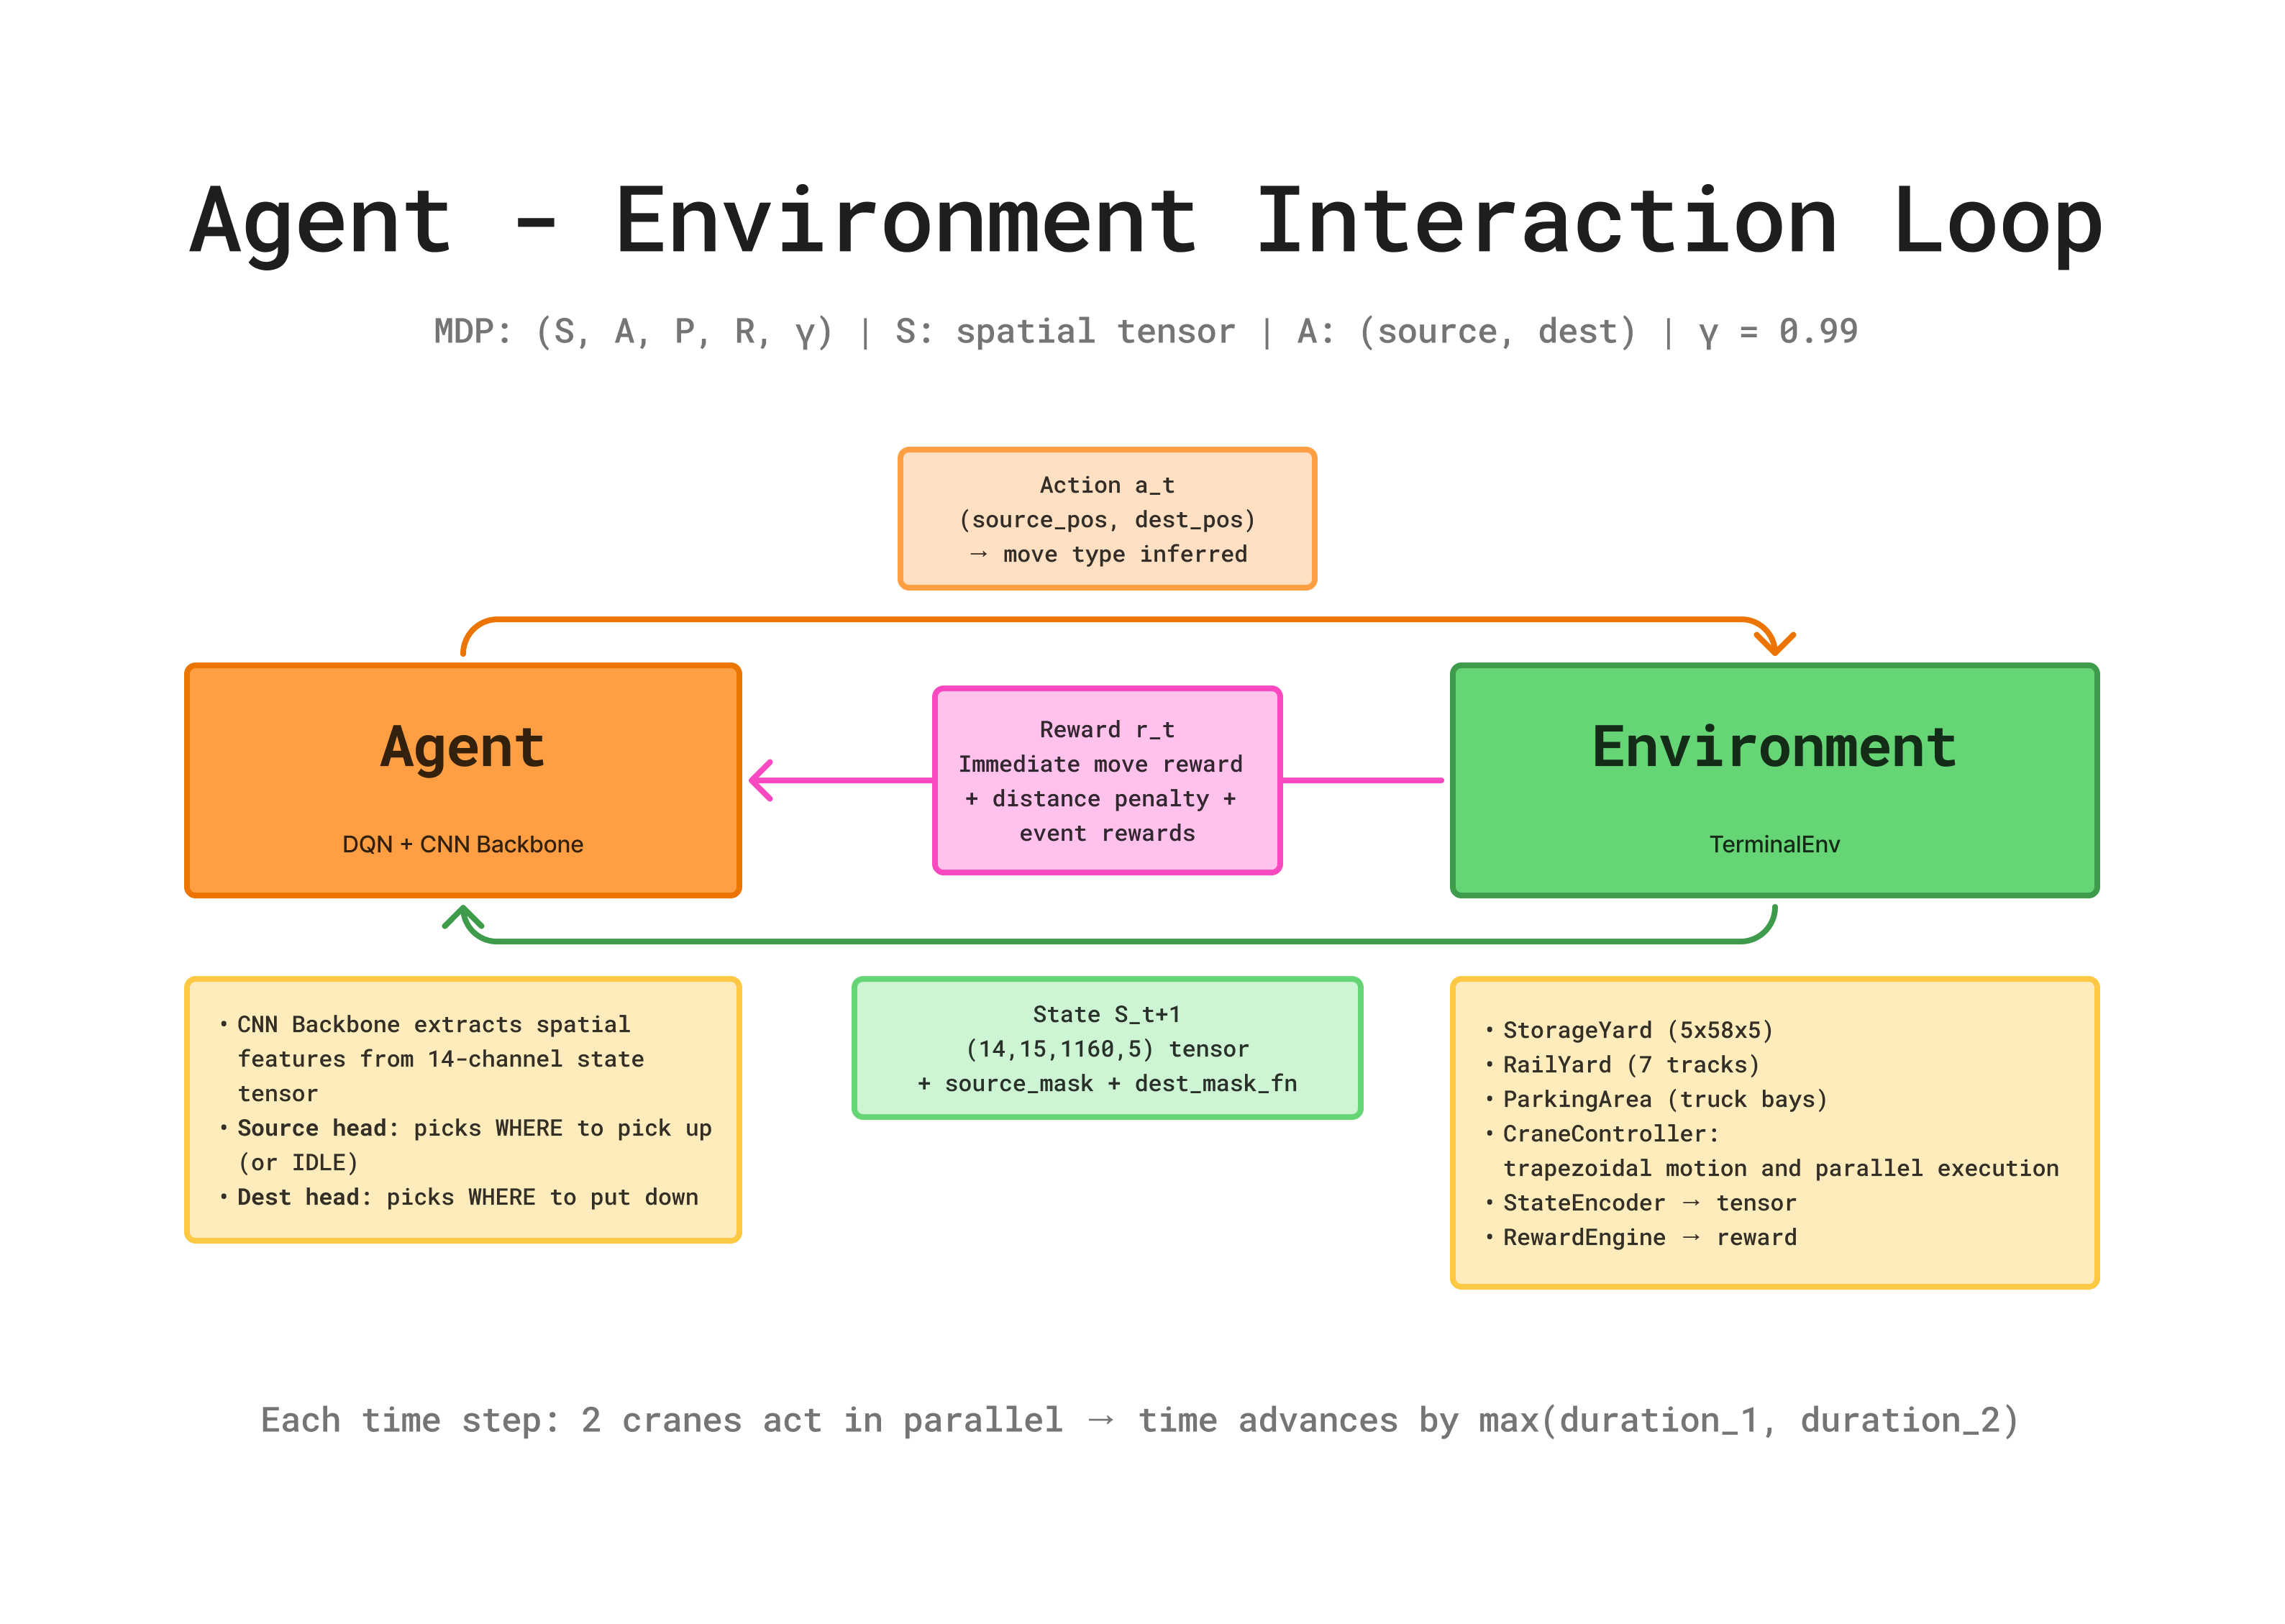
\includegraphics[width=0.85\textwidth]{mdp_loop}
  \caption{The agent--environment interaction loop instantiated for the container terminal domain. The agent observes a spatial state tensor, selects a source--destination move via its two-head CNN architecture, and receives a reward from the terminal simulation.}
  \label{fig:bg:mdp_loop}
\end{figure}

\subsection{Value-Based Methods}
\label{sec:bg:rl:value}

Value-based methods learn $\qfunc^*(\state, \action)$ and derive a greedy policy $\policy(\state) = \arg\max_\action \qfunc^*(\state, \action)$ \cite{suttonbarto2018}. Temporal-difference (TD) learning\footnote{TD learning updates value estimates from the difference between the current estimate and a one-step lookahead target, rather than waiting for the full episode return as in Monte Carlo methods.} updates Q-values toward a bootstrapped target \cite{sutton1988td}:
\begin{equation}
\label{eq:td}
\qfunc(\state_t, \action_t) \leftarrow \qfunc(\state_t, \action_t) + \alpha \bigl[\reward_{t+1} + \gamma \max_{\action'} \qfunc(\state_{t+1}, \action') - \qfunc(\state_t, \action_t)\bigr],
\end{equation}
where $\alpha$ is the learning rate and the bracketed quantity is the TD error $\delta_t$. Q-learning \cite{watkinsdayan1992} is the off-policy\footnote{An \emph{off-policy} algorithm can learn from transitions generated by any policy (including random exploration), not only from those generated by the current policy being optimised. This is what makes experience replay possible.} specialisation that maximises over next-state actions regardless of the behaviour policy. During training, $\varepsilon$-greedy exploration\footnote{$\varepsilon$-greedy selects a random action with probability $\varepsilon$ and the greedy action otherwise, balancing exploration of new strategies with exploitation of learned knowledge.} balances exploration and exploitation.

$n$-step returns \cite{sutton1988td} bootstrap after $n$ transitions rather than one, interpolating between TD learning and Monte Carlo estimation:
\begin{equation}
\label{eq:nstep}
G_t^{(n)} = \sum_{k=0}^{n-1} \gamma^k \reward_{t+k+1} + \gamma^n \max_{\action'} \qfunc(\state_{t+n}, \action').
\end{equation}
Larger $n$ reduces bootstrap bias at the cost of higher variance. This work uses $n = 3$ to propagate reward information across the short action chains that characterise individual container moves (\cref{sec:agent:training:loss}).

\subsection{Deep Q-Networks}
\label{sec:bg:rl:dqn}

When the state space is large or continuous, tabular storage of $\qfunc$ becomes infeasible. Deep Q-Networks (DQN) \cite{mnih2015dqn} approximate $\qfunc(\state, \action; \theta)$ with a neural network parameterised by weights $\theta$, trained to minimise the TD error between predicted and target Q-values. The key insight is that a convolutional neural network can extract spatial features directly from high-dimensional observations, learning an implicit state representation that supports value estimation without manual feature engineering.

Two mechanisms stabilise DQN training. Experience replay \cite{lin1992} stores transitions $(\state_t, \action_t, \reward_{t+1}, \state_{t+1})$ in a buffer and samples mini-batches uniformly at random, breaking the temporal correlation between consecutive training samples that would otherwise destabilise stochastic gradient descent. A target network $\qfunc(\cdot; \theta^-)$ provides the bootstrap target and is updated slowly, either by periodic copying or by Polyak averaging\footnote{Polyak averaging (also called exponential moving average) blends the online weights into the target weights at each step: $\theta^- \leftarrow \tau \theta + (1 - \tau) \theta^-$, where $\tau \ll 1$. This produces smoother target evolution than periodic hard replacement.} with a small coefficient $\tau$. The delayed update prevents the moving target problem where the network chases its own rapidly changing predictions \cite{mnih2015dqn}.

Double DQN \cite{hasselt2016ddqn} addresses the overestimation bias inherent in the max operator of \cref{eq:td} by decoupling action selection (online network: $\action^* = \arg\max_{\action'} \qfunc(\state', \action'; \theta)$) from evaluation (target network: $\qfunc(\state', \action^*; \theta^-)$). This correction is particularly important in domains with large masked action spaces, where few valid actions can amplify the overestimation effect.

Prioritised experience replay (PER) \cite{schaul2016per} replaces uniform sampling with a distribution that favours transitions with large TD errors: sampling probability is proportional to $(|\delta_i| + \epsilon)^\alpha$. Importance-sampling weights\footnote{Without correction, prioritised sampling distorts the expected gradient. Importance-sampling weights $w_i = (N \cdot p_i)^{-\beta}$ compensate for this bias, with $\beta$ annealing toward 1.0 over training.} correct the resulting distributional bias. Transitions that surprise the network receive more frequent updates, accelerating learning on rare but informative events such as train departures.

\subsection{Factored and Multi-Head Action Spaces}
\label{sec:bg:rl:factored}

When the action space is a Cartesian product of discrete dimensions, flat enumeration becomes intractable. A factored decomposition selects each dimension sequentially, reducing the effective count from $|\mathcal{A}_1| \times |\mathcal{A}_2|$ to $|\mathcal{A}_1| + |\mathcal{A}_2|$, with each selection conditioned on the previous ones \cite{suttonbarto2018}. The two-head\footnote{A \emph{head} is an output branch of a neural network. A multi-head architecture shares a common feature extractor (the backbone) but splits into separate output layers, each producing predictions for a different sub-task.} architecture in this work applies this principle: source selection followed by conditioned destination selection (\cref{sec:agent:unified:heads}).

A complementary decomposition operates along the value dimension. The dueling architecture \cite{wang2016dueling} separates the Q-value into a state-value stream $V(\state)$, which captures how good it is to be in a given state regardless of the action taken, and an advantage stream $A(\state, \action)$, which captures the relative benefit of each action: $\qfunc(\state, \action) = V(\state) + A(\state, \action) - \frac{1}{|\mathcal{A}|}\sum_{\action'} A(\state, \action')$. This separation is useful when many actions in a state have similar values and the critical information lies in the few that deviate from the mean.

\section{Convolutional Neural Networks for Spatial Domains}
\label{sec:bg:cnn}

Convolutional neural networks (CNNs) extract spatial features from grid-structured inputs through learned filters\footnote{A convolutional filter (or kernel) is a small weight matrix that is applied at every position of the input via element-wise multiplication and summation. Each filter learns to detect a specific local pattern --- e.g.\ an edge, a texture, or, in this work, a stacking configuration.} that slide across the input dimensions \cite{lecun1998}. Translation equivariance\footnote{A pattern detected at one spatial position is recognised equally at any other position, because the same filter weights are applied everywhere.} ensures that stacking relationships and proximity patterns are recognised regardless of bay position \cite{goodfellow2016}. Stacking multiple layers increases the effective receptive field\footnote{The receptive field is the region of the input that influences a given neuron's output. Deeper layers have larger receptive fields because each layer aggregates information from a local neighbourhood, and these neighbourhoods compose across layers.}, allowing deeper layers to capture progressively larger spatial relationships.

Group normalisation \cite{wu2020groupnorm} is preferred over batch normalisation in RL because the small batch sizes (typically 32 transitions) make batch statistics unreliable; group normalisation normalises within fixed channel groups independently of batch size.

The DQN approach to Atari demonstrated that multi-channel spatial tensors serve as effective CNN inputs for RL \cite{mnih2015dqn}. Each channel encodes a different semantic attribute (occupancy, type, urgency) at every position. When the domain has three physical dimensions, 3D convolutions \cite{ji20133dcnn} learn features along all axes simultaneously. The specific tensor layout used in this work is described in \cref{ch:state}.

\section{Curriculum Learning}
\label{sec:bg:curriculum}

Curriculum learning presents tasks in order of increasing difficulty \cite{bengio2009curriculum}. Starting with easier examples guides the optimiser into favourable regions of parameter space from which harder examples can be learned more efficiently, improving both convergence speed and final performance.

In reinforcement learning, the curriculum takes the form of progressively harder environments. The agent masters basic skills before encountering the full target complexity \cite{bengio2009curriculum}. This is particularly valuable when the target task has sparse or delayed rewards that make learning from scratch impractical, because simpler stages provide denser feedback that bootstraps useful behaviours. The explicit curriculum used in this work --- 33 tutorial scenarios across 14 difficulty tiers (\cref{ch:curriculum}) --- directly addresses the feasibility question of \cref{sec:intro:rqs}: each tier combines sub-tasks into progressively more complex compositions, building from single-move primitives to near-production terminal operations.

% chapters/03_related_work.tex
\chapter{Related Work}
\label{ch:related}

This chapter surveys the most relevant prior work across four areas: operations research for container terminal optimisation, reinforcement learning for container terminal operations, CNN-based spatial state representations in RL, and curriculum learning for RL. It concludes by identifying the research gap that this thesis addresses.

\section{Operations Research at Container Terminals}
\label{sec:rw:or}

The dominant approach to container terminal optimisation has historically been operations research. \textcite{vis2003transshipment} classify the decision problems that arise at container terminals --- berth allocation, crane scheduling, vehicle dispatching, and stacking --- and survey the quantitative models available for each. They identify the joint vehicle-scheduling-location problem as NP-hard \cite{bish2001dispatching} and note that most practical approaches rely on decomposition heuristics rather than exact methods. \textcite{stahlbock2008operations} provide a comprehensive literature update on container terminal optimisation, organising the work by subsystem (berth allocation, storage and stacking logistics, horizontal transport) and by solution methodology (analytical models, simulation, heuristics). Both surveys conclude that integrative approaches addressing multiple terminal subsystems simultaneously remain rare, with most work targeting a single sub-problem in isolation.

For rail--road terminals specifically, \textcite{boysen2013container} survey the decision problems arising in railway yards: train scheduling (assigning trains to tracks), parking position assignment (positioning containers in the yard), load planning (positioning containers on outbound trains), crane-area assignment, and crane sequencing. They distinguish direct moves (container transferred straight from train to truck) from split moves (routed through intermediate storage) and note that the operational process must address all five sub-problems jointly. The existing OR literature, however, treats them independently, using mixed-integer programming for storage and loading decisions and heuristic rules for crane scheduling. No prior OR approach solves all five jointly, which is the gap that the DRL agent in this thesis attempts to fill with a single learned policy.

\section{Reinforcement Learning for Container Terminals}
\label{sec:rw:rl}

\textcite{lai2024rl} provide a bibliometric analysis of 1{,}030 RL papers in transportation research (1996--2023), categorising them into seven application areas. Freight transportation accounts for only 5\% of the total, far behind vehicle motion planning (28\%), energy-efficient driving (20\%), and adaptive traffic signal control (19\%). Within the freight category, most work addresses autonomous ship or autonomous train path tracking rather than terminal-internal container handling. The survey identifies DQN as the most commonly used algorithm for discrete action spaces in transportation, supporting the algorithm family choice in this thesis, and highlights the sim-to-real gap as a key open challenge.

\textcite{colak2025rl} provide a more focused survey of 71 studies applying RL specifically to container terminal operations. The surveyed work spans berth allocation, quay crane scheduling, yard management, and horizontal transport. The majority of approaches use tabular Q-learning or simple policy gradient methods, and nearly all address a single operational sub-problem in isolation. The survey identifies a lack of work on jointly optimising multiple terminal operations within a single agent and highlights inland intermodal terminals as underrepresented compared to maritime ports.

\textcite{jin2024container} apply deep RL to truck dispatching in a container port, using a spatial-attention-based agent trained via a Real2Sim pipeline grounded in real port data. Their work demonstrates that DRL can handle the stochastic, real-time nature of vehicle dispatching in a terminal setting, but their scope is limited to a single operational task (truck assignment) rather than the joint crane--truck--train coordination addressed in this thesis.

In the broader logistics domain, \textcite{nazari2018vrp} apply RL with an attention-based encoder to the capacitated vehicle routing problem, removing the recurrent component of the original Pointer Network in favour of a simpler element-wise embedding. Their work demonstrates that end-to-end RL can match or exceed classical heuristics on combinatorial logistics tasks. The use of a learned encoder over spatial inputs is conceptually similar to the CNN-based state representation developed here, though their domain lacks the stacking and restacking dynamics that characterise container yards.

\section{Spatial State Representations in RL}
\label{sec:rw:cnn}

The use of CNNs as spatial feature extractors for RL was established by \textcite{mnih2015dqn}, who demonstrated human-level Atari performance by processing raw pixel frames through convolutional layers. AlphaGo \cite{silver2016go} extended this principle to a structured board game, encoding the $19 \times 19$ Go board as a multi-channel spatial tensor where each channel represents a different game-state feature (stone positions, liberties, capture history). The CNN then extracts spatial patterns that inform both policy and value prediction.

The container terminal state representation developed in this thesis follows the same multi-channel spatial paradigm. Rather than pixels or board positions, each channel encodes a semantic yard attribute (occupancy, container type, departure urgency, demand) at every spatial position across a 3D grid of rows, bays, and tiers (\cref{ch:state}). The key architectural difference is the use of 3D convolutions \cite{ji20133dcnn} to capture the volumetric stacking structure, whereas Atari and Go use 2D convolutions over flat grids.

\section{DQN Algorithm Variants}
\label{sec:rw:dqn}

Since the original DQN, several algorithmic improvements have been proposed. Double DQN \cite{hasselt2016ddqn} reduces overestimation bias. Prioritised experience replay \cite{schaul2016per} focuses training on surprising transitions. Dueling networks \cite{wang2016dueling} separate state-value and advantage estimation. NoisyNet \cite{fortunato2018noisy} replaces $\varepsilon$-greedy exploration with learned parametric noise. QR-DQN \cite{dabney2018distributional} and IQN \cite{dabney2018implicit} model the full return distribution. Munchausen DQN \cite{vieillard2020munchausen} adds a scaled log-policy bonus to the reward, implicitly regularising the policy. Spectral normalisation \cite{miyato2018spectral}, originally proposed for GANs, constrains weight matrix norms and has been adopted in RL to stabilise training.

\textcite{hessel2018rainbow} combine six of these extensions into a single Rainbow agent and perform ablation studies showing that no single extension dominates across all Atari games. This finding motivates the empirical variant screening conducted in this thesis (\cref{ch:experiments}), where seven algorithm variants are evaluated on the domain-specific tutorial curriculum rather than relying on benchmark rankings from unrelated domains.

\section{Curriculum Learning in RL}
\label{sec:rw:curriculum}

\textcite{bengio2009curriculum} introduced curriculum learning as a training strategy that presents examples in order of increasing difficulty. \textcite{narvekar2020curriculum} survey its application to RL, categorising approaches by how the curriculum is generated (hand-designed vs.\ automatic), what is sequenced (tasks, environments, reward shaping), and how transfer between stages is achieved. They note that hand-designed curricula are effective when domain knowledge is available to define a meaningful difficulty ordering, which is the case for container terminal operations where atomic moves are strictly simpler than multi-step logistics chains.

More recent work has explored automatic curriculum generation, where the training environment co-evolves with the agent. Prioritised Level Replay \cite{jiang2021plr} selectively revisits training levels based on estimated learning potential, while adversarial environment design methods generate progressively harder configurations without manual specification. These approaches are most effective in domains with parametric environment generators (e.g.\ procedural maze generation), where the difficulty space is continuous and high-dimensional. In contrast, the container terminal domain has a small, discrete set of operationally meaningful task types (nine move types, each with clear prerequisites), making a hand-designed curriculum both feasible and interpretable. The curriculum in this thesis is hand-designed with 33 scenarios across 14 difficulty tiers (\cref{ch:curriculum}), leveraging domain knowledge to define a difficulty ordering that mirrors real operational training. It additionally serves as an architecture screening tool, exploiting the correlation between tutorial learnability and full-simulation performance to reduce the computational cost of architecture search.

\section{Research Gap}
\label{sec:rw:gap}

The central question of this thesis --- whether joint terminal control is learnable by a single DRL agent (\cref{sec:intro:rqs}) --- is unanswered by any prior work. \Cref{tab:rw:gap} summarises the positioning. The OR surveys \cite{vis2003transshipment,stahlbock2008operations,boysen2013container} document extensive work on individual terminal sub-problems but no integrated solution. Recent DRL work has begun addressing individual terminal sub-problems: \textcite{jin2023stacking} apply self-attention-based DRL to container stacking optimisation, \textcite{li2023twin} use DRL with dynamic masked self-attention for twin automated stacking crane scheduling, and \textcite{jin2024container} combine Real2Sim transfer with DRL for truck dispatching. On the integration front, \textcite{naeem2023integrated} provide a comprehensive review of joint quay crane, AGV, and yard crane scheduling, while \textcite{xu2021integrated} combine RL-based hyper-heuristics with genetic algorithms for multi-equipment scheduling. However, all of these address maritime port operations, and none jointly optimises crane scheduling, truck parking, and train loading with a single agent.

The RL surveys \cite{lai2024rl,colak2025rl} confirm that freight terminal RL remains a nascent area (5\% of RL-transport publications) and that joint multi-task optimisation has not been attempted for inland terminals. No prior work uses a volumetric CNN encoding for inland terminal state representation, and no prior approach employs a tiered tutorial curriculum both for agent training and architecture screening in this domain. The curriculum design is directly motivated by this gap: by decomposing the joint problem into learnable sub-tasks and then recombining them, the curriculum tests whether compositional mastery of sub-problems translates into joint-problem competence.

\begin{table}[H]
  \centering
  \caption{Positioning of this thesis relative to prior work. Checkmarks indicate features present in each approach.}
  \label{tab:rw:gap}
  \begin{tabular}{@{} l c c c c @{}}
    \toprule
    & \textbf{Joint ops} & \textbf{CNN state} & \textbf{Curriculum} & \textbf{Inland} \\
    \midrule
    \textcite{vis2003transshipment}    & --   & --   & --   & -- \\
    \textcite{stahlbock2008operations} & --   & --   & --   & -- \\
    \textcite{boysen2013container}     & --   & --   & --   & \checkmark \\
    \textcite{colak2025rl} (survey)    & --   & --   & --   & partial \\
    \textcite{lai2024rl} (survey)      & --   & --   & --   & -- \\
    \textcite{jin2024container}        & --   & \checkmark & --   & -- \\
    \textcite{jin2023stacking}         & --   & \checkmark & --   & -- \\
    \textcite{li2023twin}              & --   & \checkmark & --   & -- \\
    \textcite{naeem2023integrated}     & partial & --   & --   & -- \\
    \textcite{xu2021integrated}        & partial & --   & --   & -- \\
    \textcite{nazari2018vrp}           & --   & --   & --   & -- \\
    \textcite{mnih2015dqn}             & n/a  & \checkmark & --   & n/a \\
    \textbf{This thesis}               & \checkmark & \checkmark & \checkmark & \checkmark \\
    \bottomrule
  \end{tabular}
\end{table}

% chapters/04_system_design.tex
\chapter{System Design}
\label{ch:system}

This chapter presents the simulation platform, the data foundation that drives it, and the action and reward formulations that connect the environment to the reinforcement learning agent.

\section{System Overview}
\label{sec:sys:overview}

The system follows a four-layer architecture, shown in \cref{fig:sys:architecture}. The bottom layer is the data foundation: scenario definitions, train schedules, and truck arrival generators derived from operational records. Above it, the environment layer implements a discrete-event simulation of an intermodal container terminal with storage yards, rail tracks, a parking area, and rail-mounted gantry cranes (RMGCs). The agent layer contains the unified spatial DQN that selects source and destination positions for container moves. The top layer is a curriculum trainer that orchestrates multi-day episodes, adjusts scenario difficulty, and manages the replay buffer. Each layer communicates through well-defined interfaces. The agent architecture is described in \cref{ch:agent}, the state representation in \cref{ch:state}, and the curriculum training strategy in \cref{ch:curriculum}.

\begin{figure}[H]
  \centering
  \resizebox{0.95\textwidth}{!}{% system_architecture.tex — Four-layer system architecture diagram (comprehensive)
% \input from Ch.4

\definecolor{SteelBlue}{HTML}{4682B4}
\definecolor{LayerTraining}{HTML}{4472C4}
\definecolor{LayerEnv}{HTML}{548235}
\definecolor{LayerOps}{HTML}{2E7D32}
\definecolor{LayerAgent}{HTML}{BF8F00}
\definecolor{LayerData}{HTML}{757575}
\definecolor{TrainingBg}{HTML}{D6E4F0}
\definecolor{EnvBg}{HTML}{E2EFDA}
\definecolor{AgentBg}{HTML}{FFF2CC}
\definecolor{DataBg}{HTML}{E8E8E8}
\definecolor{CoreBg}{HTML}{F0E6F6}
\definecolor{LayerCore}{HTML}{7B1FA2}

\begin{tikzpicture}[
    font=\small,
    % Box styles
    tbox/.style={rectangle, rounded corners=3pt, draw=LayerTraining!80!black,
        fill=LayerTraining, text=white, font=\small\bfseries,
        minimum height=0.7cm, minimum width=2.8cm, align=center},
    tbox2/.style={rectangle, rounded corners=3pt, draw=LayerTraining!60!black,
        fill=LayerTraining!65, text=white, font=\footnotesize\bfseries,
        minimum height=0.55cm, minimum width=2.0cm, align=center},
    ebox/.style={rectangle, rounded corners=3pt, draw=LayerEnv!80!black,
        fill=LayerEnv, text=white, font=\small\bfseries,
        minimum height=0.7cm, minimum width=2.8cm, align=center},
    ebox2/.style={rectangle, rounded corners=3pt, draw=LayerEnv!60!black,
        fill=LayerEnv!70, text=white, font=\footnotesize\bfseries,
        minimum height=0.6cm, minimum width=2.2cm, align=center},
    ebox3/.style={rectangle, rounded corners=3pt, draw=LayerOps!50!black,
        fill=LayerOps!55, text=white, font=\scriptsize\bfseries,
        minimum height=0.5cm, minimum width=1.8cm, align=center},
    abox/.style={rectangle, rounded corners=3pt, draw=LayerAgent!80!black,
        fill=LayerAgent!90, text=white, font=\small\bfseries,
        minimum height=0.7cm, minimum width=2.6cm, align=center},
    abox2/.style={rectangle, rounded corners=3pt, draw=LayerAgent!60!black,
        fill=LayerAgent!65, text=white, font=\footnotesize\bfseries,
        minimum height=0.55cm, minimum width=2.2cm, align=center},
    abox3/.style={rectangle, rounded corners=3pt, draw=LayerAgent!50!black,
        fill=LayerAgent!45, text=white, font=\scriptsize\bfseries,
        minimum height=0.45cm, minimum width=1.6cm, align=center},
    dbox/.style={rectangle, rounded corners=3pt, draw=LayerData!80!black,
        fill=LayerData, text=white, font=\small\bfseries,
        minimum height=0.7cm, minimum width=2.4cm, align=center},
    dbox2/.style={rectangle, rounded corners=3pt, draw=LayerData!60!black,
        fill=LayerData!60, text=white, font=\footnotesize\bfseries,
        minimum height=0.55cm, minimum width=2.0cm, align=center},
    cbox/.style={rectangle, rounded corners=3pt, draw=LayerCore!60!black,
        fill=LayerCore!55, text=white, font=\footnotesize\bfseries,
        minimum height=0.55cm, minimum width=1.8cm, align=center},
    % Grouping
    grp/.style={rectangle, rounded corners=2pt, draw=gray!40, dashed,
        inner sep=4pt},
    grplabel/.style={font=\tiny\itshape, text=gray!60!black},
    % Arrow styles
    dep/.style={-Stealth, gray!55, line width=0.5pt},
    dataflow/.style={-Stealth, dashed, SteelBlue!80!black, line width=0.9pt},
]

% ══════════════════════════════════════════════════════════════════
% Layer backgrounds
% ══════════════════════════════════════════════════════════════════
\fill[TrainingBg, rounded corners=5pt] (-7.5,  8.8) rectangle (7.5, 6.4);
\fill[EnvBg, rounded corners=5pt]      (-7.5,  5.9) rectangle (7.5, -0.2);
\fill[AgentBg, rounded corners=5pt]    (-7.5, -0.7) rectangle (7.5, -4.8);
\fill[DataBg, rounded corners=5pt]     (-7.5, -5.3) rectangle (7.5, -7.8);

% Layer labels (left margin)
\node[rotate=90, font=\footnotesize\bfseries, text=LayerTraining!80!black,
    anchor=south] at (-7.9, 7.6) {Training};
\node[rotate=90, font=\footnotesize\bfseries, text=LayerEnv!80!black,
    anchor=south] at (-7.9, 2.85) {Environment};
\node[rotate=90, font=\footnotesize\bfseries, text=LayerAgent!80!black,
    anchor=south] at (-7.9, -2.75) {Agent};
\node[rotate=90, font=\footnotesize\bfseries, text=LayerData!80!black,
    anchor=south] at (-7.9, -6.55) {Data};

% ══════════════════════════════════════════════════════════════════
% TRAINING LAYER
% ══════════════════════════════════════════════════════════════════
\node[tbox, minimum width=3.2cm] (ct) at (-2.5, 8.0) {CurriculumTrainer};
\node[tbox, minimum width=2.6cm] (tr) at (2.0, 8.0) {TutorialRunner};
\node[tbox2] (ml) at (5.5, 8.0) {MetricsLogger};
\node[tbox2] (tt) at (-2.5, 7.0) {TutorialTier};

\draw[dep] (ct) -- (tr);
\draw[dep] (ct) -- (tt);
\draw[dep] (ct) -- (ml);

% Scenario group
\node[tbox2, minimum width=2.4cm] (sc) at (2.0, 7.0) {TutorialScenario};
\node[grplabel, anchor=west] at (3.6, 7.0) {\texttimes\,33 implementations};
\draw[dep] (tr) -- (sc);

% ══════════════════════════════════════════════════════════════════
% ENVIRONMENT LAYER
% ══════════════════════════════════════════════════════════════════

% Main env
\node[ebox, minimum width=3.2cm] (env) at (0, 5.2) {TerminalEnv};
\draw[dep] (ct.south) -- ++(0,-0.3) -| (env.north);

% Core components row
\node[ebox2, minimum width=2.2cm] (se) at (-5.5, 3.7) {StateEncoder};
\node[ebox2, minimum width=2.2cm] (re) at (-2.2, 3.7) {RewardEngine};
\node[ebox2, minimum width=3.0cm] (fc) at (1.5, 3.7) {FacilityCoordinator};
\node[ebox2, minimum width=2.4cm] (cc) at (5.2, 3.7) {CraneController};

\draw[dep] (env) -- (se);
\draw[dep] (env) -- (re);
\draw[dep] (env) -- (fc);
\draw[dep] (env.east) -| (cc);

% Facilities sub-row
\node[ebox3, minimum width=2.0cm] (sy) at (-0.2, 2.4) {StorageYard};
\node[ebox3, minimum width=1.6cm] (ry) at (1.9, 2.4) {RailYard};
\node[ebox3, minimum width=2.0cm] (pa) at (3.8, 2.4) {ParkingArea};
\draw[dep] (fc) -- (sy);
\draw[dep] (fc) -- (ry);
\draw[dep] (fc) -- (pa);

% Operations sub-group
\node[ebox3, minimum width=2.8cm] (tlm) at (-4.5, 1.3) {TerminalLogisticsManager};
\node[ebox3, minimum width=2.0cm] (rmgc) at (-1.0, 1.3) {TerminalRMGC};
\node[ebox3, minimum width=1.8cm] (gate) at (1.5, 1.3) {TerminalGate};
\draw[dep] (env.south) ++(0,0) -- ++(0,-0.3) -| (tlm.north);
\draw[dep] (env.south) -- ++(0,-0.3) -| (rmgc.north);
\draw[dep] (env.south) -- ++(0,-0.3) -| (gate.north);

% Domain objects group
\node[ebox3, minimum width=1.6cm] (cont) at (3.5, 0.5) {Container};
\node[ebox3, minimum width=1.2cm] (train) at (5.0, 0.5) {Train};
\node[ebox3, minimum width=1.2cm] (truck) at (6.3, 0.5) {Truck};
\node[ebox3, minimum width=1.2cm] (wagon) at (5.0, -0.0) {Wagon};
\draw[dep] (train.south) -- (wagon.north);

\node[grplabel] at (5.0, 1.0) {core domain};

% ══════════════════════════════════════════════════════════════════
% AGENT LAYER
% ══════════════════════════════════════════════════════════════════

% Main agent
\node[abox, minimum width=3.4cm] (agent) at (-4.0, -1.5) {BaseSpatialDQNAgent};

% Variant agents (grouped)
\node[abox2, minimum width=1.8cm] (dqna) at (-6.0, -2.7) {DQNAgent};
\node[abox2, minimum width=1.8cm] (duel) at (-3.8, -2.7) {Dueling};
\node[abox2, minimum width=1.8cm] (noisy) at (-1.6, -2.7) {NoisyNet};
\node[abox3, minimum width=1.5cm] (qrdqn) at (-6.0, -3.5) {QR-DQN};
\node[abox3, minimum width=1.3cm] (iqn) at (-4.5, -3.5) {IQN};
\node[abox3, minimum width=1.7cm] (munch) at (-2.8, -3.5) {Munchausen};
\node[abox3, minimum width=1.8cm] (ks) at (-1.1, -3.5) {KitchenSink};

\draw[dep] (agent) -- (dqna);
\draw[dep] (agent) -- (duel);
\draw[dep] (agent) -- (noisy);
\draw[dep] (agent.south) ++(0,0) -- ++(0, -0.35) -| (qrdqn);
\draw[dep] (agent.south) -- ++(0, -0.35) -| (iqn);
\draw[dep] (agent.south) -- ++(0, -0.35) -| (munch);
\draw[dep] (agent.south) -- ++(0, -0.35) -| (ks);

\node[grplabel] at (-3.5, -4.2) {7 DQN variants};

% Network components
\node[abox2, minimum width=3.2cm] (qnet) at (3.5, -1.5)
    {QNetwork};
\node[abox3, minimum width=2.6cm] (cnn) at (1.8, -2.5) {CNNBackbone};
\node[abox3, minimum width=1.8cm] (src) at (4.0, -2.5) {SourceHead};
\node[abox3, minimum width=1.6cm] (dst) at (5.8, -2.5) {DestHead};
\node[abox3, minimum width=2.2cm] (idle) at (4.0, -3.3) {IdleSourceWrapper};

\draw[dep] (qnet) -- (cnn);
\draw[dep] (qnet) -- (src);
\draw[dep] (qnet) -- (dst);
\draw[dep] (src) -- (idle);

\node[abox2, minimum width=2.2cm] (rb) at (3.5, -4.2) {ReplayBuffer};
\draw[dep] (agent.east) -- ++(0.5,0) |- (qnet.west);
\draw[dep] (agent.east) -- ++(0.5,0) |- (rb.west);

\node[grplabel] at (1.8, -3.2) {6 backbone variants};

% ══════════════════════════════════════════════════════════════════
% DATA LAYER
% ══════════════════════════════════════════════════════════════════

% Scheduling and generation
\node[dbox, minimum width=2.4cm] (tsch) at (-4.5, -5.9) {TrainScheduler};
\node[dbox2, minimum width=2.2cm] (tload) at (-4.5, -6.9) {TrainLoader};
\node[dbox, minimum width=2.4cm] (lm) at (-1.0, -5.9) {LogisticsManager};
\node[dbox2, minimum width=1.8cm] (dp) at (-1.0, -6.9) {DayPlan};

\draw[dep] (tsch) -- (tload);
\draw[dep] (lm) -- (dp);

% Generators
\node[dbox, minimum width=2.4cm] (tgen) at (2.8, -5.9) {TruckGenerator};

% Factories
\node[dbox2, minimum width=2.4cm] (cfac) at (5.8, -5.9) {ContainerFactory};
\node[dbox2, minimum width=2.0cm] (tfac) at (5.8, -6.9) {TruckFactory};

\draw[dep] (tgen) -- ++(0,-0.5) -| (tfac);

\node[grplabel] at (5.8, -7.4) {factories};

% Config
\node[dbox2, minimum width=2.2cm] (cfg) at (2.8, -6.9) {Config};
\node[grplabel, anchor=west] at (4.1, -6.9) {\scriptsize (12 dataclasses)};

% Data → Env connections
\draw[dep] (tsch.north) -- ++(0, 1.5) -| ([xshift=-1.2cm]env.south);
\draw[dep] (lm.north) -- ++(0, 1.0) -| ([xshift=-0.3cm]env.south);
\draw[dep] (tgen.north) -- ++(0, 0.5) -| ([xshift=0.6cm]env.south);

% ══════════════════════════════════════════════════════════════════
% DATA FLOW ARROWS (dashed blue)
% ══════════════════════════════════════════════════════════════════

% State tensor: StateEncoder → Agent
\draw[dataflow]
    (se.south) -- ++(0,-1.2)
    -| node[pos=0.20, below, font=\scriptsize, text=SteelBlue!70!black,
        fill=white, inner sep=1pt, fill opacity=0.85, text opacity=1]
        {state tensor $(14,\!15,\!1160,\!5)$}
    ([xshift=0.8cm]agent.north);

% Masks: Env → Agent
\draw[dataflow]
    ([xshift=-1.2cm]env.south) -- ++(0,-0.5)
    -| node[pos=0.12, left, font=\scriptsize, text=SteelBlue!70!black,
        fill=white, inner sep=1pt, fill opacity=0.85, text opacity=1] {masks}
    ([xshift=-0.5cm]agent.north);

% Action: Agent → Env (going right and up)
\draw[dataflow]
    ([xshift=1.5cm]agent.north) -- ++(0,0.6)
    -| node[pos=0.20, above, font=\scriptsize, text=SteelBlue!70!black,
        fill=white, inner sep=1pt, fill opacity=0.85, text opacity=1]
        {action (src, dest)}
    ([xshift=1.5cm]env.south);

\end{tikzpicture}
}
  \caption{System architecture showing the four layers (Training, Environment, Agent, Data) and their class dependencies. Dashed arrows indicate data flow: the state tensor $(14, 15, 1{,}160, 5)$ flows from the state encoder to the agent, which returns a source--destination action pair.}
  \label{fig:sys:architecture}
\end{figure}

A single simulation step proceeds as follows. The environment first processes pending arrivals and departures, collecting event-driven rewards such as train departure bonuses or truck waiting penalties. It then identifies all idle cranes, encodes the terminal state into a multi-channel spatial tensor, passes it to the agent, and receives back a source and destination position. The \texttt{TerminalLogisticsManager} validates and executes the resulting container move, the \texttt{TerminalRMGC} computes the crane travel cost in metres and seconds, and an immediate reward is assembled from a type-specific bonus plus distance and time penalties. When multiple cranes act within the same step, the simulation clock advances by the longest individual crane duration, reflecting parallel operation.

\section{Simulation Environment}
\label{sec:sys:env}

\subsection{Terminal Model}
\label{sec:sys:env:model}

The physical terminal is represented by the \texttt{StorageYard}, which models a block-stacking yard with 5 rows, 58 bays, and 5 tiers. Each bay is subdivided by a split factor of 20, yielding sub-slots of 2 feet each ($58 \times 20 = 1{,}160$ split positions per row). This sub-bay granularity allows containers of seven standardised lengths (20, 22, 23, 24, 30, 40, and 45 feet) to share bays without wasted space, following the binary encoding principle of \cite{caserta2009binary}. The primary data structure is a 3D NumPy integer array of shape \texttt{(n\_tiers, n\_rows, total\_splits)} that maps each coordinate to a container index, enabling O(1) occupancy lookups.

The rail infrastructure (\texttt{RailYard}) manages 7 tracks. Each train maps to a track through a slot object that records an anchor bay position, linking the train's location to the yard's coordinate system. The parking infrastructure (\texttt{ParkingArea}) uses the same bay-and-split grid. The state representation arranges all regions into 15 contiguous rows, detailed in \cref{ch:state}. \Cref{fig:sys:terminal_layout} shows the spatial arrangement of all facility regions, including the crane zones.

\begin{figure}[H]
  \centering
  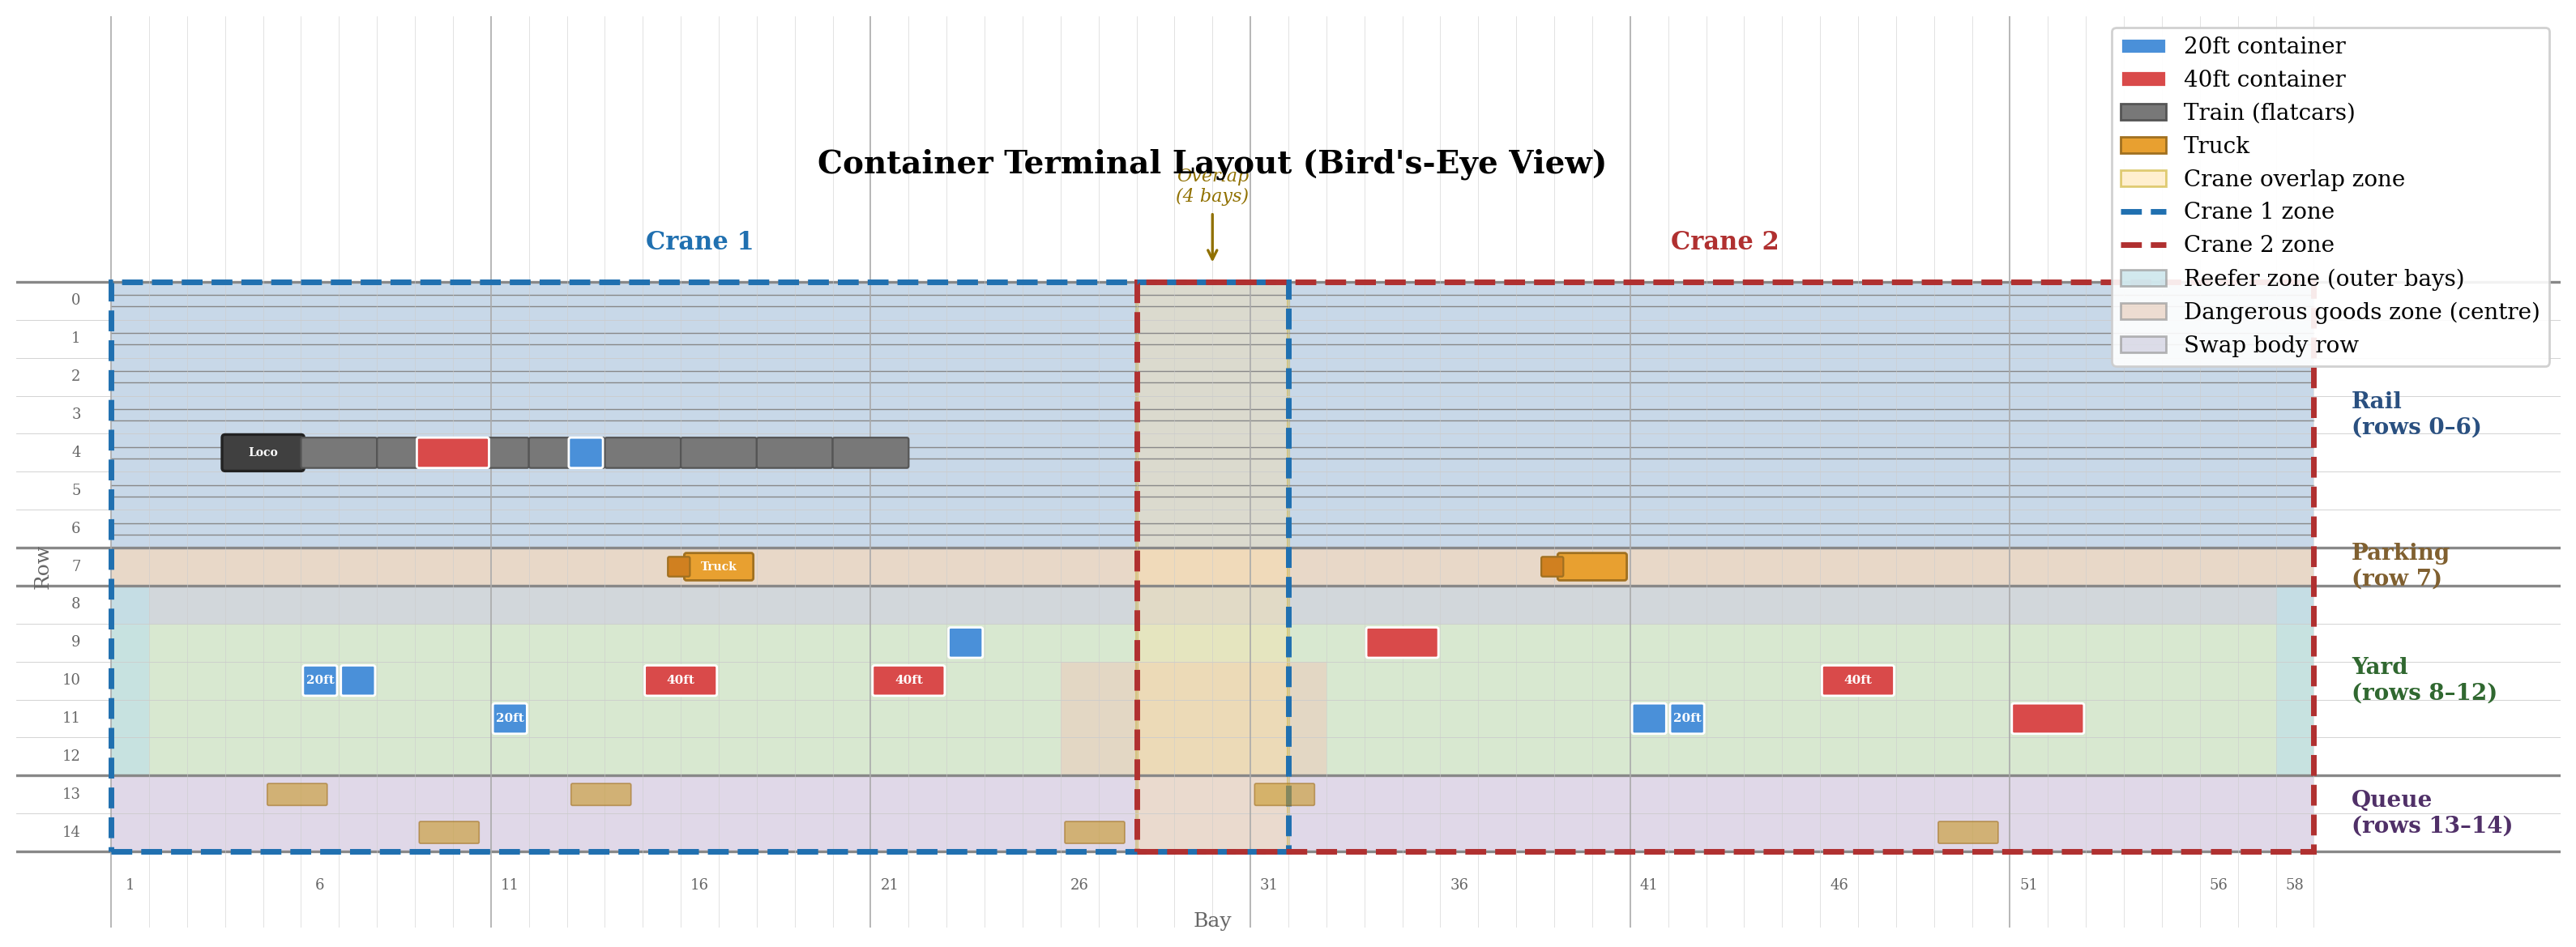
\includegraphics[width=\textwidth]{terminal_layout}
  \caption{Bird's-eye view of the terminal layout. The 58-bay axis runs horizontally. Rows 0--6 are rail tracks, row~7 is parking, rows~8--12 are the storage yard, and rows~13--14 are the truck queue. Two cranes (blue dashed, red dashed) operate in overlapping zones with a 4-bay overlap region (amber).}
  \label{fig:sys:terminal_layout}
\end{figure}

\subsection{Container and Vehicle Models}
\label{sec:sys:env:entities}

Every container is characterised by a direction (Import or Export), physical dimensions, a goods type (Regular, Reefer, or DangerousGoods), and arrival and departure dates. Reefer containers require powered positions at the yard's outer bays, dangerous goods must be placed in designated central zones, and swap bodies are restricted to ground-level storage. These constraints are enforced through Boolean masks baked into the yard at initialisation, ensuring that the agent can only place containers in valid positions.

A \texttt{Train} consists of wagons, each capable of holding multiple containers up to its length capacity, and carries a pickup manifest listing container IDs to collect before departure. The train lifecycle progresses through arriving, waiting, loading, departing, and departed. The \texttt{TrainScheduler} assigns trains to tracks using a best-fit decreasing heuristic, sorted by dwell duration.

A \texttt{Truck} either delivers export containers or arrives with a pickup manifest to collect imports. Truck arrival times are sampled from day-of-week-specific KDE\footnote{Kernel density estimation: a non-parametric method that estimates a continuous probability distribution from discrete data points by placing a smooth kernel (here Gaussian) at each observation.} models, producing the bimodal peak pattern (morning and afternoon surges) observed at real terminals.

\subsection{Logistics and Planning Layer}
\label{sec:sys:env:logistics}

The \texttt{LogisticsManager} constructs daily traffic plans by querying KDE-based arrival distributions for truck counts and timings, while train arrivals follow a weekly schedule parsed from a driving plan JSON. The export-to-import ratio defaults to 0.75, drawn from N\"urnberg TriCon statistics, with a daily cap of 220 import containers via rail.

The \texttt{ContainerFactory} samples container lengths and goods types from operator-specific probability tables fitted to the N\"urnberg dataset. The \texttt{TerminalLogisticsManager} is the move execution engine: it validates agent-selected source--destination pairs against the current terminal state, updates entity positions, and returns a success or failure flag.

\subsection{Crane Movement Model}
\label{sec:sys:env:rmgc}

The \texttt{TerminalRMGC} computes the physical cost of every crane operation. Given source and destination positions, it resolves each to 3D coordinates (X along bays, Y across rows, Z for tier height) and computes travel time with a trapezoidal motion profile for each axis independently. The critical-path time is the maximum across the three axes, plus a fixed 30-second handling time for container lock and unlock, consistent with the positioning time reported by \textcite{stahlbock2008operations} for RMG operations. The total cost feeds directly into the reward function.

The 58-bay gantry axis is partitioned into overlapping zones (one per crane, 4-bay overlap) for concurrent multi-crane operation. When multiple idle cranes are dispatched within a single step, a per-step blacklist prevents one crane from reversing a move made by another in the same step (\cref{sec:state:masking:blacklist}).

\subsection{Time Model}
\label{sec:sys:env:time}

The simulation uses an operation-driven time model. When multiple cranes execute moves within a single \texttt{step\_all\_cranes()} call, the clock advances by the \emph{longest} individual crane duration rather than their sum, reflecting the physical reality that cranes in separate zones work simultaneously. A typical two-crane step advances the clock by 120 to 300 seconds. When no valid moves exist and all cranes are idle, a fixed 30-second increment allows pending arrivals or departures to resolve.

A day begins with \texttt{env.reset()}, which loads a traffic plan with optional carryover entities from the previous day. The day ends when the clock reaches 23:59 or the step count reaches 5{,}000. End-of-day penalties are applied for stacking inversions and leftover containers, and unfinished trains or trucks carry over to the next day.

\section{Data Foundation}
\label{sec:sys:data}

The simulation is calibrated to operational data from the N\"urnberg TriCon intermodal terminal. The dataset contains container arrival patterns, dwell time distributions, the mix of container sizes across operators, goods-type frequencies, and weekly train schedules. Truck arrival profiles are derived from timestamped gate logs stratified by day of week. Gaussian kernel density estimates fitted to these logs produce stochastic arrivals that are statistically consistent with reality yet never identical across episodes, providing the variation needed for robust policy training.

\section{Action Space Design}
\label{sec:sys:actions}

\subsection{Move Types}
\label{sec:sys:actions:types}

The simulation supports nine operational move types plus a learnable \texttt{IDLE} action, summarised in \cref{tab:sys:move_types}. Eight of these are \emph{container} move types involving crane operations; the ninth (\texttt{YARD\_TO\_T.TRUCK}) dispatches containers to terminal trucks and is exercised only in Phase~1 tutorials. The move type is not an explicit agent decision but is inferred deterministically from the spatial regions of the selected source and destination through a fixed lookup table.

\begin{table}[H]
  \centering
  \caption{Move types supported by the simulation. Each type is inferred from the source and destination regions of the agent's spatial selection.}
  \label{tab:sys:move_types}
  \begin{tabular}{@{} l l l l @{}}
    \toprule
    \textbf{Move Type} & \textbf{Source} & \textbf{Destination} & \textbf{Description} \\
    \midrule
    \texttt{PARK\_TRUCK}      & Queue   & Parking & Park a truck in a free spot \\
    \texttt{TRAIN\_TO\_YARD}  & Rail    & Yard    & Unload import from wagon \\
    \texttt{TRUCK\_TO\_YARD}  & Parking & Yard    & Transfer export from truck \\
    \texttt{YARD\_TO\_YARD}   & Yard    & Yard    & Restack within the yard \\
    \texttt{YARD\_TO\_TRAIN}  & Yard    & Rail    & Load export onto train \\
    \texttt{YARD\_TO\_TRUCK}  & Yard    & Parking & Place import onto pickup truck \\
    \texttt{TRAIN\_TO\_TRUCK} & Rail    & Parking & Direct transfer, bypasses yard \\
    \texttt{TRUCK\_TO\_TRAIN} & Parking & Rail    & Direct transfer, bypasses yard \\
    \texttt{YARD\_TO\_T.TRUCK}& Yard    & Queue   & Dispatch to terminal truck \\
    \midrule
    \texttt{IDLE}             & \multicolumn{2}{l}{Learnable source position} & Deliberate wait \\
    \bottomrule
  \end{tabular}
\end{table}

\begin{figure}[H]
  \centering
  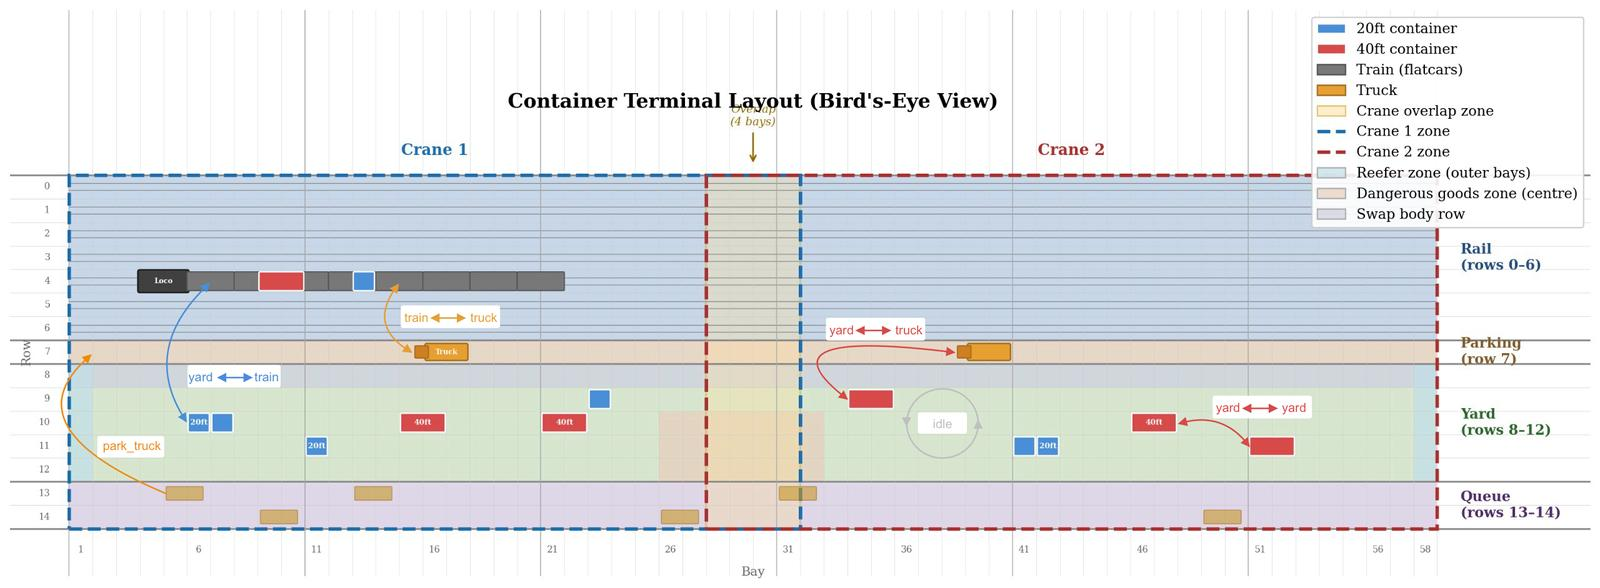
\includegraphics[width=0.9\textwidth]{move_types_layout}
  \caption{View of the terminal layout showing the four facility regions and the nine move types as directed arrows. Solid arrows represent productive container transfers; the circular IDLE action represents a deliberate wait.}
  \label{fig:sys:move_types}
\end{figure}

\subsection{Unified Source--Destination Formulation}
\label{sec:sys:actions:unified}

The agent's action consists of two sequential decisions: select a source position (row, split, tier) in the unified 15-row grid, then select a destination in the same coordinate space. This replaces a naive flat enumeration that would yield $15 \times 1{,}160 \times 5 = 87{,}000$ positions per decision.

Both decisions are constrained by dynamic masks that encode the full logistics logic of the terminal, as described next.

\section{Source and Destination Masking}
\label{sec:state:masking}

The masks are the mechanism through which domain constraints enter the action space. Invalid action masking \cite{huang2022masking} sets the Q-values of physically impossible actions to $-\infty$ before selection, ensuring the agent never wastes experience on impossible moves and every exploratory action produces a meaningful transition.

\subsection{Source Mask Construction}
\label{sec:state:masking:source}

The source mask is a boolean tensor of shape $(R_\text{uni}, S, T)$ that marks every position from which the agent may select a source entity. In the yard rows, a position is marked if the container is accessible (topmost in its stack) and the position is the container's start split. On rail rows, only Import containers are marked, using the container's immutable \texttt{direction} attribute as described in \cref{sec:state:channels:structure}. In the parking row, only delivery trucks carrying Export containers are marked. In the queue rows, all waiting trucks are marked as valid sources for the parking action.

\subsection{Destination Mask Function}
\label{sec:state:masking:dest}

The destination mask is not a static tensor but a function of the selected source position. The environment pre-computes a yard validity mask that checks occupancy, support conditions, and contiguous free space for each possible placement, along with a parking free-slot mask. The closure \texttt{\_make\_dest\_mask\_fn()} then applies region-dependent logic based on where the source was selected.

If the source is in the queue rows, valid destinations are free parking positions. If the source is on a rail row or in the parking row, valid destinations are open yard positions that satisfy the container's goods-type placement rules. If the source is in the yard, valid destinations include other yard positions for restacking, plus direction-dependent vehicle targets. For Export yard containers, the mask includes rail wagon positions on tracks where a train has requested that specific container and has space for it. For Import yard containers, the mask includes parking positions of trucks whose pickup manifest contains that container's ID. This conditional masking encodes the full logistics logic of the terminal directly into the action space, relieving the agent from learning which region combinations are valid through trial and error.

\subsection{Anti-Reversal Blacklist}
\label{sec:state:masking:blacklist}

In a multi-crane terminal, two cranes operating within the same \texttt{step\_all\_cranes()} call could reverse each other's moves. Crane 1 might move container A from the yard to a rail wagon, and crane 2 might immediately move it back. The anti-reversal blacklist prevents this by maintaining a per-step set of container IDs that have been moved during the current step. Before the second crane's source mask is computed, the blacklist is applied to zero out positions occupied by recently moved containers.

The blacklist is scoped to a single step rather than an entire episode. A container moved in step $n$ becomes available again in step $n + 1$ because the intervening time may change the operational context and make the container a legitimate target. This per-step scope was chosen after the multi-crane reversal bug was discovered during tutorial scenario debugging, where bidirectional train flows (Tier 7 and above) repeatedly triggered the reversal pattern. The resolution is discussed in \cref{sec:disc:engineering}.

\section{Reward Engineering}
\label{sec:sys:reward}

\subsection{Immediate Move Rewards}
\label{sec:sys:reward:immediate}

Every executed move receives an immediate reward composed of a type-specific bonus and a distance-plus-time cost. The bonuses, listed in \cref{tab:sys:move_rewards}, encode operational priority. The distance component applies $-0.001$ per metre of crane travel and the time component adds $-0.0005$ per second, deliberately small relative to type bonuses to create a gradient toward efficient placements without overriding the priority signal.

\begin{table}[H]
  \centering
  \caption{Immediate move rewards. Higher bonuses reflect higher operational urgency.}
  \label{tab:sys:move_rewards}
  \begin{tabular}{@{} l r l @{}}
    \toprule
    \textbf{Move Type} & \textbf{Bonus} & \textbf{Rationale} \\
    \midrule
    \texttt{YARD\_TO\_TRAIN}  & $+7.0$ & Most time-critical (delays departure) \\
    \texttt{TRUCK\_TO\_TRAIN} & $+7.0$ & Direct export, same urgency \\
    \texttt{TRAIN\_TO\_TRUCK} & $+5.0$ & Direct import, bypasses yard \\
    \texttt{YARD\_TO\_TRUCK}  & $+3.0$ & Customer service (truck waiting) \\
    \texttt{TRAIN\_TO\_YARD}  & $+2.5$ & Import unloading \\
    \texttt{TRUCK\_TO\_YARD}  & $+0.8$ & Export staging \\
    \texttt{PARK\_TRUCK}      & $+0.1$ & Low priority, plus proximity bonus$^{*}$ \\
    \texttt{YARD\_TO\_YARD}   & $-0.2$ & Discourages unnecessary reshuffling \\
    \texttt{IDLE}             & $-0.1$ & Penalises inaction \\
    \midrule
    Distance cost             & \multicolumn{2}{l}{$-0.001$ per metre of crane travel} \\
    Time cost                 & \multicolumn{2}{l}{$-0.0005$ per second of crane time} \\
    \bottomrule
    \multicolumn{3}{@{}l}{\footnotesize $^{*}$Up to $+0.5$ additional, decaying linearly over 5 bays from the cargo's zone anchor.}
  \end{tabular}
\end{table}

\subsection{Event-Driven Rewards}
\label{sec:sys:reward:events}

Event-driven rewards are issued at key milestones, summarised in \cref{tab:sys:event_rewards}. A continuous per-truck-per-minute waiting penalty was initially included but was disabled after evaluation revealed it overwhelmed the learning signal (see \cref{app:reward:corrections}). The reward magnitudes were calibrated iteratively during development: the ordering reflects operational priority, and the absolute values were tuned so that multi-step sequences yield net positive return only when they complete a meaningful logistics chain.

\begin{table}[H]
  \centering
  \caption{Event-driven rewards issued at milestones during the simulation.}
  \label{tab:sys:event_rewards}
  \begin{tabular}{@{} l r l @{}}
    \toprule
    \textbf{Event} & \textbf{Reward} & \textbf{Condition} \\
    \midrule
    Train departure (success)   & $+10.0$ & All manifest containers loaded \\
    Train departure (per miss)  & $-3.0$  & Per manifest container not loaded \\
    Truck served promptly       & $+2.0$  & Service within 60 minutes \\
    Truck served late           & $+2.0 \to 0.0$ & Linear decay, 60--180 min \\
    \midrule
    Stacking inversion (end-of-day) & $-0.5$ & Per inversion in yard \\
    Overdue container (end-of-day) & $-0.3$ & Per container past departure date \\
    \bottomrule
  \end{tabular}
\end{table}

The reward hierarchy mirrors the operational phasing documented by \textcite{boysen2013container}: shortly after a train's arrival, direct moves from train to waiting trucks are processed first (rewarded at $+5.0$ for \texttt{TRAIN\_TO\_TRUCK}); next, wagon-to-storage moves predominate ($+2.5$ for \texttt{TRAIN\_TO\_YARD}); finally, storage-to-truck retrieval completes the chain ($+3.0$ for \texttt{YARD\_TO\_TRUCK}). The $+7.0$ bonus for \texttt{YARD\_TO\_TRAIN} reflects the operational reality that export loading is the most time-critical move type, since unfinished loads delay train departures. The negative reward for \texttt{YARD\_TO\_YARD} ($-0.2$) reflects the finding that reshuffles are ``unproductive container movements'' \cite{vis2003transshipment} --- necessary to unlock buried containers but costly in crane time and therefore to be minimised. The full reward specification is given in \cref{app:reward}.

\medskip

Together, the simulation environment, data foundation, action formulation, and reward design form the Markov decision process that the reinforcement learning agent must solve. The next two chapters describe how this MDP is observed (\cref{ch:state}: the spatial state tensor) and acted upon (\cref{ch:agent}: the two-head DQN architecture).

% chapters/05_state_representation.tex
\chapter{Unified Spatial State Representation}
\label{ch:state}

At each decision step the agent receives a single snapshot of the entire terminal: every container, truck, train wagon, and queue position encoded as a multi-channel spatial tensor. This chapter describes the design of that tensor --- the rationale behind the unified grid, its geometric layout, the 14 channels that populate it, and the region-specific rules that translate domain objects into activations. The masking logic that constrains action selection is described alongside the action space in \cref{sec:state:masking}.

\section{Design Rationale}
\label{sec:state:rationale}

The operational decisions in a container terminal are fundamentally spatial. A train at bay~10 is relevant to a container at bay~12 and a truck parked at bay~11, because loading that container requires minimal crane travel when the three entities are close together. Flat feature vectors destroy this structure by collapsing all positions into an unordered list. A spatial tensor preserves geometric relationships and allows convolutional filters to learn local patterns such as proximity, alignment, and blocking.

The key design principle is \emph{unification}. Rather than encoding trains, trucks, yard containers, and queued vehicles in separate data structures, the encoder places every entity into a single three-dimensional grid sharing the same bay, split, and tier axes. The CNN's cross-region kernel (\cref{sec:agent:unified:cnn}) can then bridge adjacent rows in a single forward pass, discovering associations such as the relationship between an export container in the yard and the train wagon that needs it one row above. An earlier architecture (version~6, \cref{sec:disc:architecture_evolution}) used Gaussian heat maps in separate per-region encodings to signal demand from trains and trucks, forcing the CNN to reconstruct spatial relationships from blurred overlays. The unified grid is simpler, requires fewer channels, and gives the network direct access to every entity's position.

\section{Tensor Layout}
\label{sec:state:layout}

The state tensor has shape $(C, R, S, T) = (14, 15, 1160, 5)$, using the terminal geometry described in \cref{sec:sys:env:model}. The 15 rows follow the region ordering from \cref{fig:sys:terminal_layout}: rail tracks (rows 0--6), parking (row~7), yard (rows 8--12), and queue (rows 13--14). This ordering is deliberate: regions that interact most frequently are spatial neighbours, so the cross-region kernel (\cref{sec:agent:unified:cnn}) can detect patterns between rail and yard or between parking and yard within a single receptive field.

\begin{figure}[H]
  \centering
  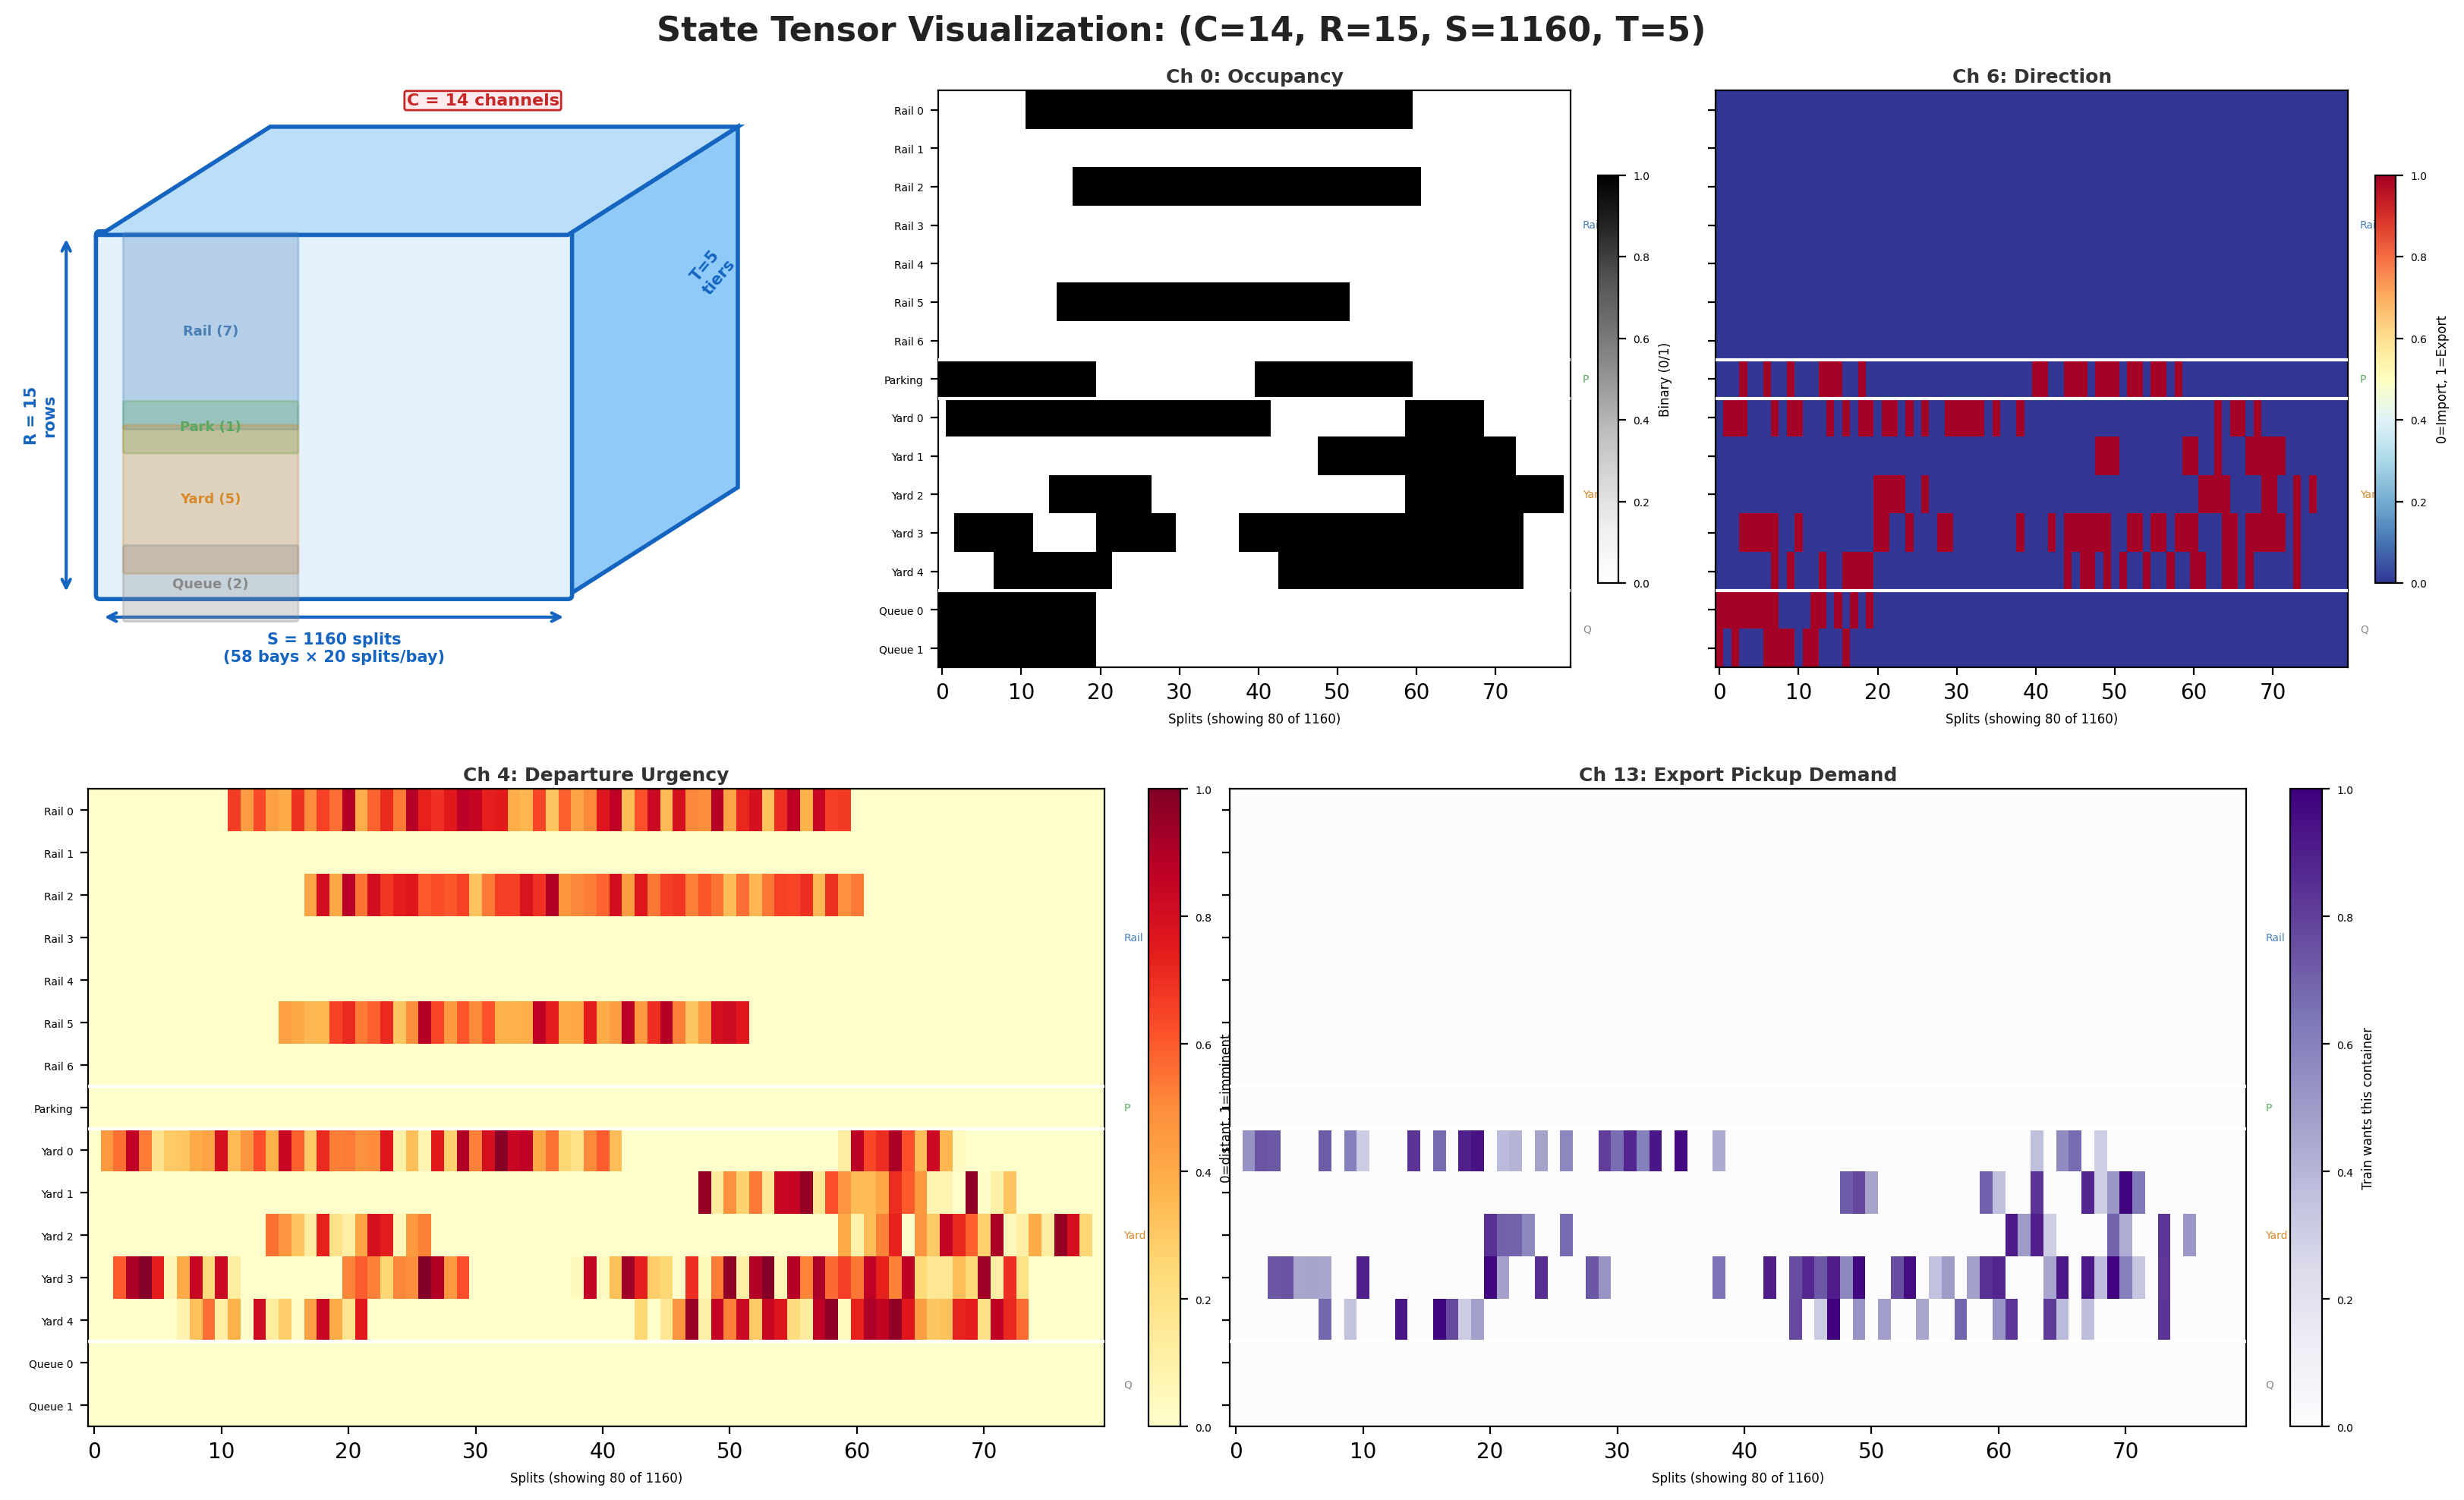
\includegraphics[width=\textwidth]{state_tensor_visualization}
  \caption{Left: the four-dimensional state tensor with region assignments along the row axis. Right: example channel activations for four representative channels.}
  \label{fig:state:tensor_viz}
\end{figure}

\section{Channel Design}
\label{sec:state:channels}

The 14 channels can be understood as answering four questions that the agent must resolve at every decision step: \emph{What is here?} (structure), \emph{How urgent is it?} (priority), \emph{Where should it go?} (demand), and \emph{What is the global context?} (coordination). \Cref{tab:state:channels} provides a compact reference; the remainder of this section explains the reasoning behind each group.

\begin{table}[H]
\centering
\caption{Summary of the 14 state tensor channels, grouped by function.}
\label{tab:state:channels}
\small
\begin{tabularx}{\textwidth}{c l l X}
\toprule
\textbf{Idx} & \textbf{Channel} & \textbf{Range} & \textbf{Description} \\
\midrule
\multicolumn{4}{@{}l}{\textit{Structure --- what is here?}} \\
\addlinespace[2pt]
0  & OCCUPANCY            & $\{0, 1\}$    & 1 if split is occupied by a container or vehicle \\
1  & CONTAINER\_START     & $\{0, 1\}$    & 1 at the leftmost split of each container \\
2  & CONTAINER\_TYPE      & $[0, 1]$      & Goods type: regular=0.25, reefer=0.50, DG=0.75, swap=1.0 \\
3  & ACCESSIBLE           & $\{0, 1\}$    & 1 if container is topmost in its stack (accessible) \\
6  & DIRECTION            & $\{0, 0.5, 1\}$ & Import=0, terminal truck=0.5, Export=1 \\
7  & CONTAINER\_HASH      & $[0.1, 1.0]$  & Unique per-container identifier (stable across steps) \\
\midrule
\multicolumn{4}{@{}l}{\textit{Priority --- how urgent is it?}} \\
\addlinespace[2pt]
4  & DEPARTURE\_URGENCY   & $[0, 1]$      & Normalised time until departure (trucks: wait hours/4) \\
5  & BLOCKS\_URGENT       & $[0, 1]$      & Stacking inversion score (blocks a more urgent container) \\
\midrule
\multicolumn{4}{@{}l}{\textit{Demand --- where should it go?}} \\
\addlinespace[2pt]
8  & TRUCK\_DEMAND        & $[0, 1]$      & Yard positions wanted by a parked pickup truck \\
9  & TRAIN\_DEMAND        & $[0, 1]$      & Yard positions wanted by a docked train (value = normalised anchor bay) \\
13 & EXPORT\_PICKUP\_DEMAND & $[0, 1]$    & Urgency-weighted flag for containers on trains' pickup lists \\
\midrule
\multicolumn{4}{@{}l}{\textit{Coordination --- what is the global context?}} \\
\addlinespace[2pt]
10 & CRANE\_PROXIMITY     & $[0, 1]$      & Triangular decay from crane's current bay position \\
11 & TRAIN\_DEPARTURE\_URG & $[0, 1]$     & Time remaining / total stay duration for each train \\
12 & TIME\_PROGRESS       & $[0, 1]$      & Seconds since midnight / 86\,400 (global clock signal) \\
\bottomrule
\end{tabularx}
\end{table}

\paragraph{Structure (channels 0--3, 6--7).}
\label{sec:state:channels:structure}
The first group tells the network what occupies each position. The binary \texttt{OCCUPANCY} mask (ch.~0) provides the coarsest signal. \texttt{CONTAINER\_START} (ch.~1) refines it by marking only the leftmost split of each container, letting the CNN distinguish two adjacent containers from a single multi-split one. \texttt{CONTAINER\_TYPE} (ch.~2) encodes the goods category as a categorical float (regular\,=\,0.25, reefer\,=\,0.50, dangerous goods\,=\,0.75, swap body\,=\,1.0), since placement constraints depend on goods type (\cref{sec:sys:env:entities}). \texttt{ACCESSIBLE} (ch.~3) flags containers that are topmost in their stack and can be picked up without restacking. The CNN can overlay this information with the demand channels to identify which wanted containers are immediately reachable and which require a restack first.

\texttt{DIRECTION} (ch.~6) encodes the container's flow direction: Import\,=\,0, Export\,=\,1. Terminal trucks, which shuttle containers internally and have no intrinsic import/export direction, receive the midpoint value~0.5, distinguishing them from pickup trucks~(0) and delivery trucks~(1) in the parking and queue rows. This channel drives the destination masking logic (\cref{sec:state:masking:dest}): Export containers may target rail wagons, Import containers may target pickup trucks. Importantly, the encoding uses the container's immutable \texttt{direction} attribute. Finally, \texttt{CONTAINER\_HASH} (ch.~7) provides a deterministic identity value in~$[0.1, 1.0]$ computed from the entity~ID, allowing the CNN to track an individual container across steps even when it moves to a new position.

\paragraph{Priority (channels 4--5).}
\label{sec:state:channels:priority}
Two channels encode temporal urgency. \texttt{DEPARTURE\_URGENCY} (ch.~4) normalises the time remaining before an entity must leave: \newline $\min(1.0,\; \text{days\_remaining} / 30.0)$ for containers and $\min(1.0,\; \text{wait\_hours} / 4.0)$ for trucks. A value near~0 signals an imminent deadline. \texttt{BLOCKS\_URGENT} (ch.~5) captures stacking inversions: when a container at tier~$t$ sits above a more urgent container at tier~$t{-}1$, the channel records the urgency difference $u_t - u_{t{-}1}$, quantifying how badly the stack needs reshuffling. Together, these two channels let the network decide both \emph{which} containers to prioritise and \emph{which stacks} to fix first.

\paragraph{Demand (channels 8--9, 13).}
\label{sec:state:channels:demand}
The demand group answers ``where should this container go?''\ by painting target signals onto yard positions. \texttt{TRUCK\_DEMAND} (ch.~8) lights up every yard position that a parked pickup truck wants to collect (1.0 at each demanded split). \texttt{TRAIN\_DEMAND} (ch.~9) does the same for trains, but encodes the value as the normalised anchor bay of the requesting train rather than a flat~1.0 --- this provides both a demand flag and a spatial hint about the train's location, so the cross-region kernel can learn directional loading patterns.

\texttt{EXPORT\_PICKUP\_DEMAND} (ch.~13) complements channel~9 by adding urgency weighting: $\max(0.1,\; 1.0 - \min(1.0,\; \text{hours\_until\_departure} / H_\text{max}))$. Where channel~9 tells the agent \emph{which} containers a train wants, channel~13 tells it \emph{how urgently} each is needed. A container demanded by a train departing in 30 minutes will have a near-1.0 activation, while one for a train with hours to spare stays near~0.1. The combination of these three channels replaced an earlier Gaussian heat map approach with exact, position-accurate demand signals.

\paragraph{Coordination (channels 10--12).}
\label{sec:state:channels:coord}
The final group provides global context that no single entity carries. \texttt{CRANE\_PROXIMITY} (ch.~10) encodes a triangular decay from each crane's current bay position (1.0 at the crane, linearly decaying to~0.0 at the terminal edges). Because both cranes share a single channel, the CNN receives an implicit coordination signal: positions between the two cranes have overlapping activations, while positions near one crane but far from the other do not. This allows the network to learn a soft spatial partitioning without explicit crane assignment logic.

\texttt{TRAIN\_DEPARTURE\_URG} (ch.~11) gives a per-rail-row countdown: $\text{time\_remaining} / \text{total\_stay}$, where 1.0 means a train has just arrived and 0.0 means departure is imminent. Unlike the per-container urgency in channel~4, this is a row-wide broadcast that signals the train as a whole. \texttt{TIME\_PROGRESS} (ch.~12) broadcasts $\text{seconds\_since\_midnight} / 86{,}400$ uniformly across all positions, providing the only absolute temporal reference in the tensor. Since truck arrival patterns are time-of-day dependent, this channel allows the agent to implicitly learn scheduling heuristics (e.g.\ prioritise parking in the morning when truck arrivals peak).

\section{Region-Specific Encoding}
\label{sec:state:regions}

The 14 channels are shared across all regions, but each region fills them according to its own physical semantics. The mapping from domain objects to tensor activations follows the terminal geometry described in \cref{sec:sys:env:model}.

\textbf{Rail rows (0--6).} Each wagon is mapped to its bay position via the train's anchor bay plus the wagon's offset. All rail containers are marked accessible (no stacking on wagons). The demand channels mark requested containers at their \emph{yard} positions while the rail row signals the train's anchor, forming a spatial correspondence that the cross-region kernel can learn to bridge.

\textbf{Parking row (7).} Parked trucks are encoded at their allocated bay positions. The direction channel uses the actual container direction for delivery trucks and defaults to Import for pickup trucks. Departure urgency is repurposed to encode truck waiting time, creating an implicit ``serve me soon'' signal that grows over time.

\textbf{Yard rows (8--12).} The occupancy array is transposed from the yard's internal $(T, R, S)$ layout to the tensor's $(R, S, T)$ ordering so that the tier axis aligns with the CNN's depth dimension. Per-container channels are filled from the yard's records, with demand overlays from truck and train manifests applied on top. This is the most information-dense region: all 14 channels are active.

\textbf{Queue rows (13--14).} Trucks that have arrived but not yet been parked are placed at their preferred bay position (median bay of wanted containers for pickups, goods-type zone anchor for deliveries). When multiple trucks target the same bay, they stack across both queue rows. This gives the CNN a preview of incoming demand \emph{before} the parking decision is made --- a key advantage of the unified grid over separate region encodings, as the spatial proximity between a queued truck and its target containers is directly visible in the tensor.

% chapters/06_agent_architecture.tex
\chapter{Agent Architecture}
\label{ch:agent}

This chapter describes the neural network architecture that processes the unified spatial tensor (\cref{ch:state}) and produces container move decisions. The design centres on three components: a CNN backbone that extracts spatial features from the state tensor, a two-head decision structure that selects source and destination positions sequentially, and a Double DQN training procedure with prioritised experience replay.

\Cref{fig:agent:action_pipeline} provides an overview of the full pipeline. The state tensor enters the CNN backbone, which produces a shared spatial feature map. The source head scores every valid source position; after masking, the highest-scoring position is selected. Its feature vector is then injected into the destination head, which scores every valid destination position conditioned on the selected source. The move type (e.g.\ YARD\_TO\_TRAIN, TRAIN\_TO\_YARD) is inferred deterministically from the spatial regions of the two selected positions. This means that no explicit move-type prediction is needed.

\begin{figure}[H]
  \centering
  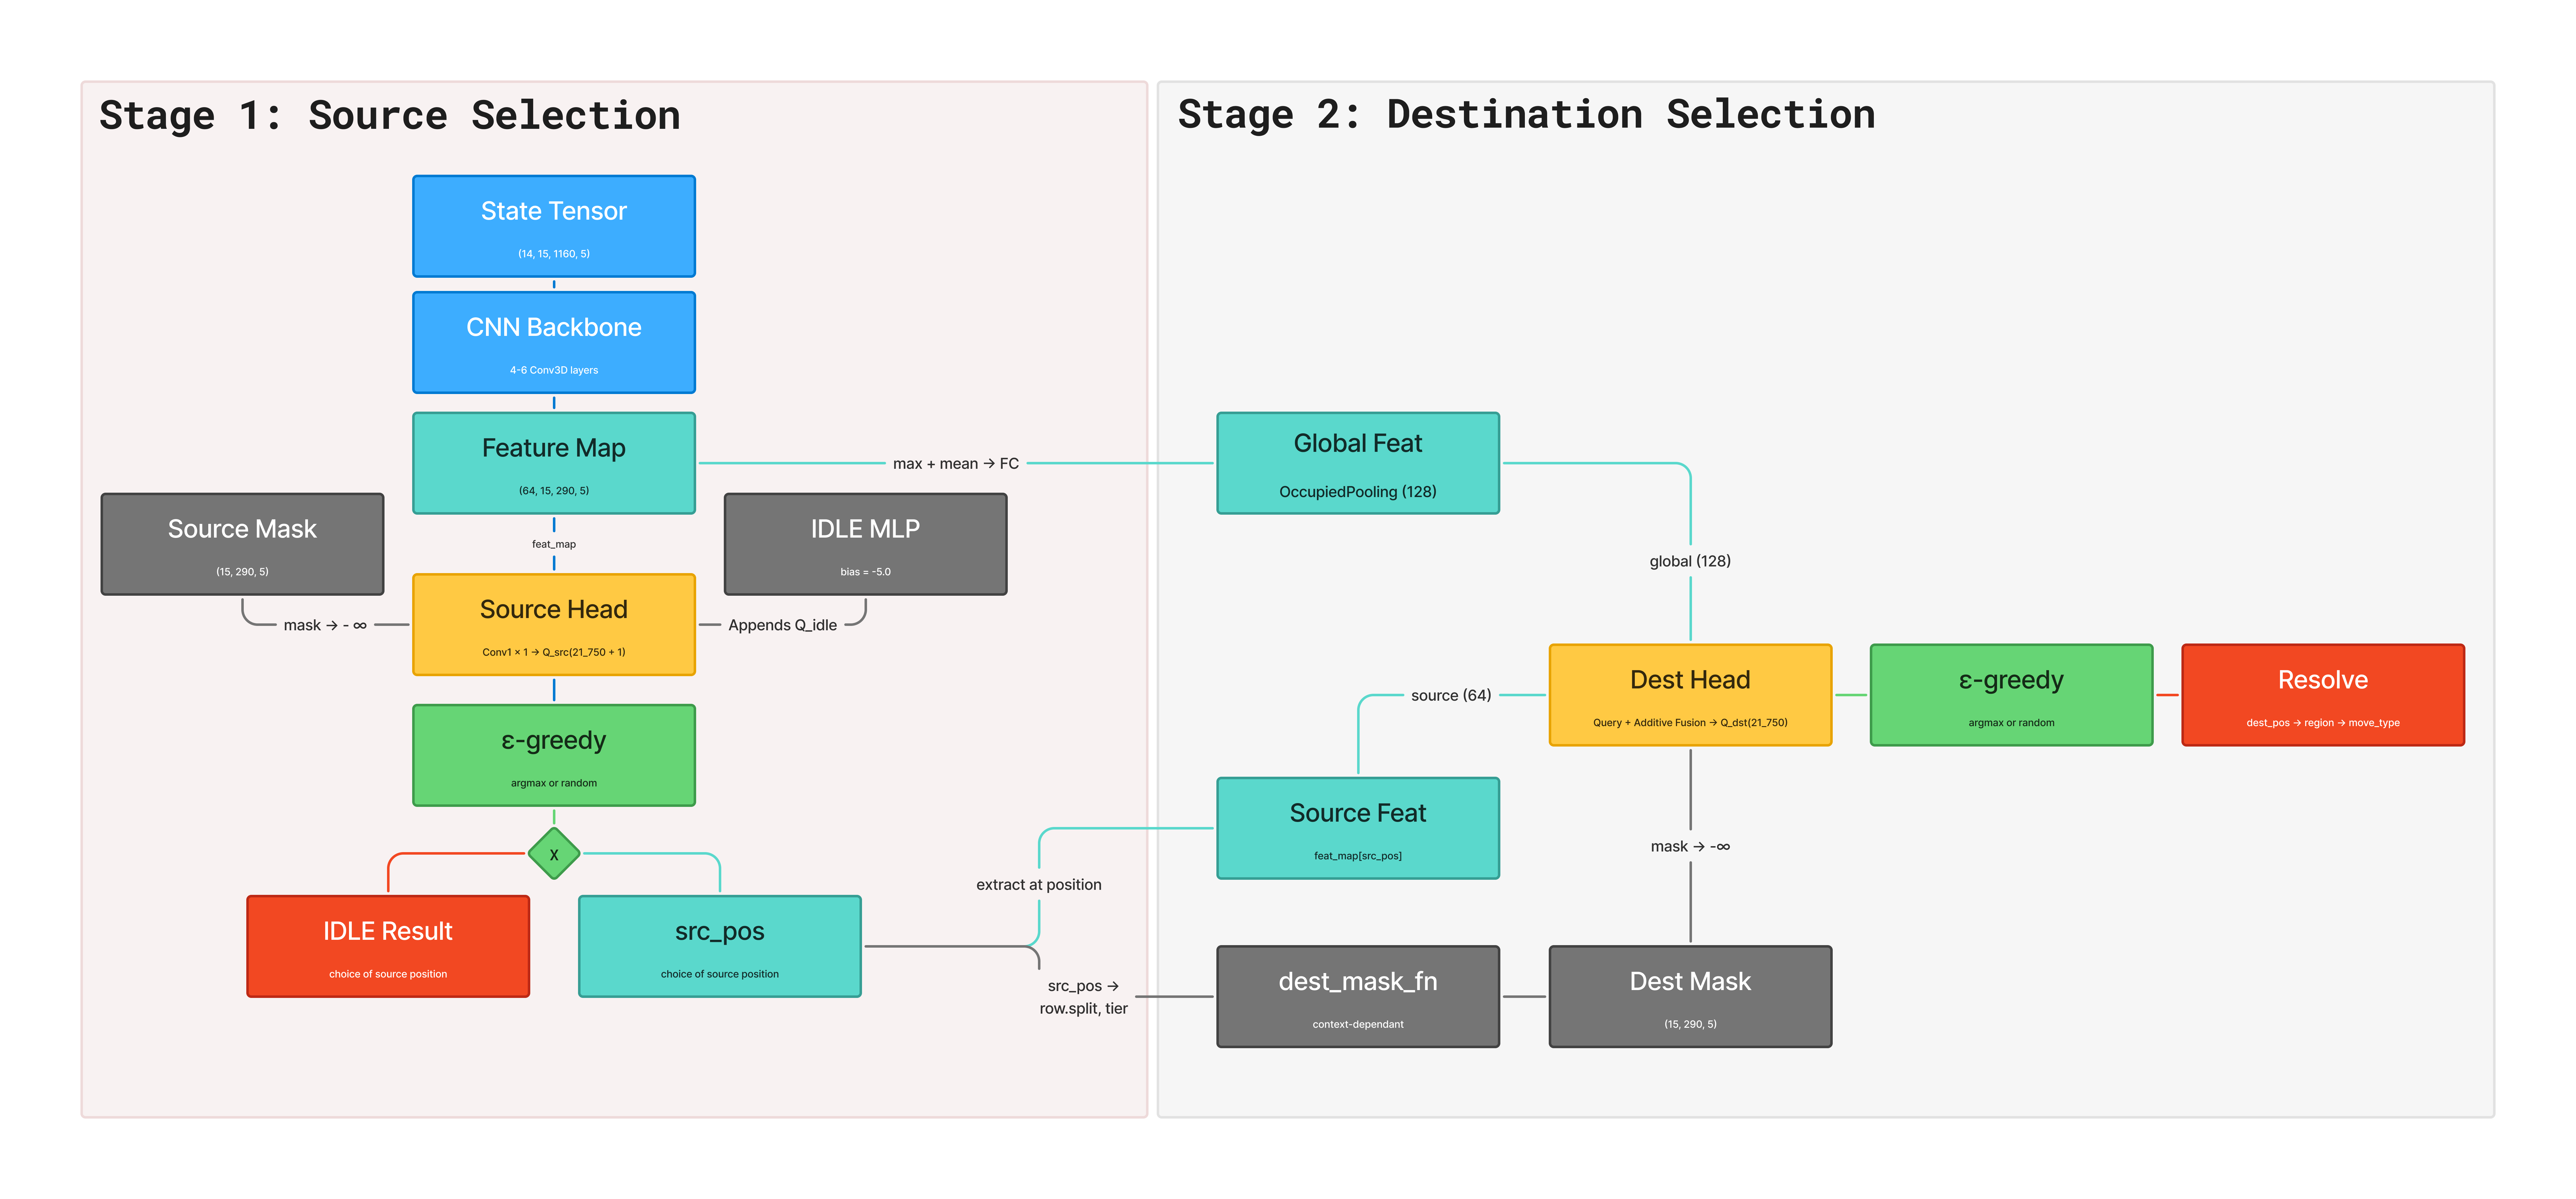
\includegraphics[width=\textwidth]{action_selection_pipeline}
  \caption{The two-stage action selection pipeline. Stage~1 selects a source position (or IDLE) from the masked source Q-values. Stage~2 conditions on the source context and selects a destination from the masked destination Q-values. The move type is inferred deterministically from the source and destination regions.}
  \label{fig:agent:action_pipeline}
\end{figure}

The remainder of this section describes each component in detail: the CNN backbone (\cref{sec:agent:unified:cnn}), the two decision heads (\cref{sec:agent:unified:heads}), and the Q-value computation that ties them together (\cref{sec:agent:unified:qvalue}).

\section{Unified DQN Agent}
\label{sec:agent:unified}

\subsection{CNN Backbone}
\label{sec:agent:unified:cnn}

The \texttt{FactoredCNNBackbone} processes the $(14, 15, 1160, 5)$ state tensor through four convolutional stages, each followed by GroupNorm\footnote{Group normalisation divides channels into groups and normalises within each group, providing stable training with small batch sizes where batch normalisation degrades.} \cite{wu2020groupnorm} with 8 groups and a ReLU activation. The kernel shapes are specifically chosen to match the terminal's spatial structure, and each stage has a distinct purpose.

\textbf{Stages 1a--1b: Bay-level feature extraction.} Stage~1a applies a $(1, 21, 1)$ kernel that spans exactly one bay (20 splits) plus one boundary position along the split axis. This acts as a \emph{container profile detector}: it learns to recognise the occupancy, type, urgency, and direction patterns within a single bay from all 14 input channels, producing 32 feature channels. Stage~1b applies the same $(1, 21, 1)$ kernel with a stride of $(1, 4, 1)$, reducing the split dimension from 1{,}160 to 290 while expanding to 64 channels. The four-fold downsampling compresses the action space from $15 \times 1{,}160 \times 5 = 87{,}000$ positions to $15 \times 290 \times 5 = 21{,}750$ positions per head. The downsampling is a deliberate trade-off to enable training on consumer hardware (8\,GB VRAM). Crucially, the downsampling is \emph{lossless} for this domain: it limits the agent's pointing precision but not its placement precision. Each downsampled position maps to a window of 4 full-resolution splits (8\,ft), and a per-step resolver searches this window to find the exact container (for sources) or the first contiguous free space that fits the container's actual size (for destinations). Since the smallest container in the simulation is 20\,ft (10 splits) --- well above the 4-split stride --- two adjacent containers always occupy distinct downsampled positions and can be independently targeted. Individual bays are still resolved (each bay spans 5 downsampled positions), and the resolver ensures that containers are packed at full resolution with no wasted space.

\textbf{Stage 2: Cross-region association.} A $(3, 1, 3)$ kernel spans 3 rows and 3 tiers simultaneously, bridging adjacent facility regions (e.g.\ rail row~6 and parking row~7, or parking row~7 and yard row~8) and adjacent tiers (detecting stacking relationships). This is the primary mechanism through which the CNN learns cross-modal spatial associations --- for instance, the proximity between a train wagon and a yard container that needs to be loaded onto it.

\textbf{Stage 3: Neighbourhood refinement.} A $(1, 5, 1)$ kernel scans along the downsampled split axis, where 5 positions span roughly 1.25 bays. This allows the network to compare containers across adjacent bays and learn local placement preferences. After all four stages the output is a feature map of shape $(64, 15, 290, 5)$ that serves as the shared representation for both decision heads.

The factored kernel design --- bay-level, then cross-region, then neighbourhood --- mirrors the decision structure of the task itself. The agent first needs to understand what is inside each bay, then how bays in different regions relate to each other, and finally how neighbouring bays compare. Two stacked $(3, 1, 3)$ kernels provide a $7 \times 3$ effective receptive field across the row dimension, large enough to span from any rail track through the parking row into the yard.

\subsection{Two-Head Decision Structure}
\label{sec:agent:unified:heads}

The agent makes two sequential decisions per simulation step. The \textbf{source head} selects an entity to move from the unified spatial grid. The \textbf{destination head}, conditioned on the selected source, selects a target position for that entity. The move type is inferred deterministically from the spatial regions of the source and destination positions (\cref{sec:sys:actions:types}), eliminating four prediction heads from the prior six-head architecture (\cref{sec:disc:architecture_evolution}).

Each head operates over the $21{,}750$ positions of the downsampled feature map. The sequential factorisation with masking keeps the effective action count small at each step: rather than choosing from $21{,}750^2 \approx 473$ million source--destination pairs, the agent makes two masked selections of at most a few hundred valid positions each. The destination head receives explicit source context (the source feature vector extracted from the CNN feature map), enabling it to learn source-dependent placement preferences. For example, placing an import container near the truck that will eventually collect it.

The two-head design also improves credit assignment: the training signal is concentrated into two spatial prediction problems rather than diluted across six separate heads, making learning dynamics more stable and easier to diagnose.

\subsection{Q-Value Computation}
\label{sec:agent:unified:qvalue}

The \texttt{OccupiedPooling} module produces a global feature vector by combining max-pooling and mean-pooling over occupied positions in the feature map, followed by a linear projection to 128 dimensions. Pooling is restricted to positions where the occupancy mask is non-zero, preventing empty space from diluting the aggregated signal. The resulting 128-dimensional vector summarises the global state of the terminal.

\textbf{Source scoring.} The source head applies two pointwise convolutions (\texttt{Conv3d(64, 32, 1)} followed by \texttt{Conv3d(32, 1, 1)}) with a ReLU activation between them, producing a scalar Q-value at each spatial position. The output is flattened to a vector of length 21{,}750 and masked so that invalid source positions receive $-\infty$. Under greedy action selection the agent picks the position with the highest Q-value; under epsilon-greedy exploration it samples uniformly from valid positions with probability $\varepsilon$.

\textbf{Destination scoring.} The destination head first constructs a query vector by projecting the concatenation of the global feature (128-d) and the source feature (64-d, extracted at the selected source position) through a linear layer to 64 dimensions. This query is broadcast-added to every position of the feature map (\emph{additive fusion}), creating an augmented feature map that encodes source-dependent context at every spatial location. The augmented map is scored with the same pointwise convolution pattern as the source head. Additive fusion allows the destination scoring to be source-conditioned without requiring a separate forward pass through the backbone for each possible source.

\Cref{alg:action_selection} formalises the two-stage action selection procedure.

\begin{algorithm}[H]
\caption{Two-Stage Spatial Action Selection}
\label{alg:action_selection}
\DontPrintSemicolon
\KwIn{State tensor $\mathbf{s} \in \mathbb{R}^{14 \times 15 \times 1160 \times 5}$, source mask $\mathbf{m}_\text{src}$, destination mask function $\texttt{dest\_mask\_fn}$, exploration rate $\varepsilon$}
\KwOut{Source position $p_\text{src}$, destination position $p_\text{dst}$, move type $t$}

$\mathbf{F} \leftarrow \texttt{CNN\_backbone}(\mathbf{s})$ \tcp*{shared feature map $(64, 15, 290, 5)$}
$\mathbf{g} \leftarrow \texttt{OccupiedPooling}(\mathbf{F})$ \tcp*{global feature vector $\in \mathbb{R}^{128}$}

\BlankLine
\tcp{Stage 1: Source selection}
$\mathbf{Q}_\text{src} \leftarrow \texttt{SourceHead}(\mathbf{F})$ \tcp*{Q-values $\in \mathbb{R}^{21750}$}
$\mathbf{Q}_\text{src}[\neg\,\mathbf{m}_\text{src}] \leftarrow -\infty$ \tcp*{mask invalid sources}
\uIf{$\text{uniform}(0,1) < \varepsilon$}{
  $p_\text{src} \leftarrow \text{uniform\_sample}(\{i : \mathbf{m}_\text{src}[i] = 1\})$\;
}
\Else{
  $p_\text{src} \leftarrow \arg\max\, \mathbf{Q}_\text{src}$\;
}

\lIf{$p_\text{src} = \texttt{IDLE}$}{\Return{$(\texttt{IDLE}, \texttt{null}, \texttt{IDLE})$}}

\BlankLine
\tcp{Stage 2: Destination selection}
$\mathbf{f}_\text{src} \leftarrow \mathbf{F}[p_\text{src}]$ \tcp*{source feature $\in \mathbb{R}^{64}$}
$\mathbf{q} \leftarrow \texttt{Linear}([\mathbf{g} \,\|\, \mathbf{f}_\text{src}])$ \tcp*{query vector $\in \mathbb{R}^{64}$}
$\mathbf{F}' \leftarrow \mathbf{F} + \mathbf{q}$ \tcp*{additive fusion (broadcast)}
$\mathbf{Q}_\text{dst} \leftarrow \texttt{DestHead}(\mathbf{F}')$\;
$\mathbf{m}_\text{dst} \leftarrow \texttt{dest\_mask\_fn}(p_\text{src})$\;
$\mathbf{Q}_\text{dst}[\neg\,\mathbf{m}_\text{dst}] \leftarrow -\infty$\;
$p_\text{dst} \leftarrow \arg\max\, \mathbf{Q}_\text{dst}$ \tcp*{greedy; $\varepsilon$-greedy analogous}

\BlankLine
$t \leftarrow \texttt{infer\_move\_type}(\text{region}(p_\text{src}),\, \text{region}(p_\text{dst}))$\;
\Return{$(p_\text{src},\, p_\text{dst},\, t)$}\;
\end{algorithm}

\section{Experience Replay}
\label{sec:agent:replay}

\subsection{Unified Transition Format}
\label{sec:agent:replay:transition}

Each transition contains the tuple (state, source\_pos\_down, dest\_pos\_down, reward, next\_state, done), where positions are recorded at the downsampled resolution ($S_\text{down} = 290$) for direct indexing into the Q-value tensors. States are compressed to float16 on storage and decompressed to float32 on sampling, with a copy-on-sample pattern to prevent in-place mutation of buffer entries.

\subsection{Prioritised Replay Buffer}
\label{sec:agent:replay:prioritised}

The prioritised variant follows \cite{schaul2016per}, assigning sampling probability proportional to $|\delta_i|^\alpha$ ($\alpha = 0.6$). Importance-sampling weights $(N \cdot p_i)^{-\beta}$ correct the distribution bias, with $\beta$ annealing from 0.4 to 1.0 over 100{,}000 frames. Priorities are clamped to a finite maximum to prevent overflow from early-training TD errors.

The buffer capacity is 3{,}000 transitions. This relatively small size reflects two constraints. First, each state tensor at float16 occupies approximately 2.3 megabytes, making large buffers memory-prohibitive. Second, terminal episodes produce highly correlated transitions within a single simulated day, and a small buffer ensures that outdated experience from previous curriculum stages is replaced quickly as the traffic intensity increases.

\section{Training Algorithm}
\label{sec:agent:training}

\subsection{Double DQN with Target Network}
\label{sec:agent:training:ddqn}

The agent uses Double DQN (\cref{sec:bg:rl:dqn}) to reduce overestimation bias. The decoupling of action selection (online network) from evaluation (target network) is particularly important in the container terminal domain because the masked action space can create spurious high Q-values at boundary positions where only one or two actions are valid, amplifying the overestimation problem.

The target network is updated via Polyak averaging (soft update) with coefficient $\tau = 0.005$ after every optimisation step. This provides smoother target evolution than periodic hard updates, which matters when the small replay buffer means the agent sees rapid distributional shift between curriculum stages. The soft update also avoids the instability spikes that hard target replacement can cause when the online network has drifted substantially between update intervals.

\subsection{Exploration Strategy}
\label{sec:agent:training:exploration}

Epsilon-greedy exploration is used during training, with schedules adapted to each training phase: a fast decay (0.9 to 0.05 over 80 epochs) for the short tutorial episodes, and a per-stage reset (1.0 to 0.05 over 50{,}000 steps) during full simulation to enable renewed exploration under new traffic conditions. Because all exploration is constrained by validity masks (\cref{sec:state:masking}), every random action produces a meaningful transition so that the agent never wastes experience on impossible moves. The NoisyNet variant replaces epsilon-greedy with learned parametric noise, enabling state-dependent exploration that adapts to local state complexity.

\subsection{Loss Function and Optimisation}
\label{sec:agent:training:loss}

The source head is trained with the standard smooth L1 (Huber) loss between the predicted Q-value of the taken source action and the bootstrapped target $r + \gamma (1 - d) \max_{a'} Q_\text{target}(s', a')$, using a discount factor of $\gamma = 0.99$ and $n$-step returns \cite{sutton1988td} with $n = 3$. The destination head uses an auxiliary loss formulation where it is trained as a reward predictor rather than a Q-value estimator. Its target is the immediate reward $r$ without bootstrapping, weighted at 0.5 relative to the source loss. This asymmetric design reflects the sequential decision structure. The source decision determines the trajectory (which entity to move), while the destination decision refines the immediate outcome (where to place it). Training the destination head on immediate rewards rather than bootstrapped returns prevents it from inheriting the source head's value estimation noise.

The optimiser is Adam with a learning rate of $3 \times 10^{-4}$, batch size of 32, and gradient clipping at a maximum norm of 1.0. The total loss per update is $\mathcal{L} = \mathcal{L}_\text{src} + 0.5 \cdot \mathcal{L}_\text{dst}$. Up to 10 additional optimisation passes are performed at the end of each tutorial epoch, proportional to the number of transitions collected during that epoch, ensuring that the network extracts maximum learning from the small replay buffer. The full set of training hyperparameters is given in \cref{app:hyperparameters}.

\Cref{alg:training_update} summarises the Double DQN parameter update with the asymmetric source--destination loss.

\begin{algorithm}[H]
\caption{Double DQN Training Update (Single Batch)}
\label{alg:training_update}
\DontPrintSemicolon
\KwIn{Replay buffer $\mathcal{B}$, online network $Q_\theta$, target network $Q_{\theta^-}$, batch size $B$, discount $\gamma$, Polyak coefficient $\tau$, $n$-step horizon $n$}

Sample batch $\{(s_i, a^\text{src}_i, a^\text{dst}_i, r_i, R^{(n)}_i, s'_i, d_i)\}_{i=1}^{B} \sim \mathcal{B}$\;

\BlankLine
\tcp{Source head: Double DQN with $n$-step returns}
$a^*_i \leftarrow \arg\max_a\, Q_\theta^\text{src}(s'_i,\, a)$ \tcp*{online selects}
$y_i^\text{src} \leftarrow R^{(n)}_i + \gamma^n (1 - d_i)\, Q_{\theta^-}^\text{src}(s'_i,\, a^*_i)$ \tcp*{target evaluates}
$\mathcal{L}_\text{src} \leftarrow \frac{1}{B} \sum_i w_i \cdot \text{SmoothL1}\!\bigl(Q_\theta^\text{src}(s_i, a_i^\text{src}),\; y_i^\text{src}\bigr)$\;

\BlankLine
\tcp{Destination head: immediate-reward auxiliary loss}
$y_i^\text{dst} \leftarrow r_i$ \tcp*{no bootstrapping}
$\mathcal{L}_\text{dst} \leftarrow \frac{1}{B} \sum_i w_i \cdot \text{SmoothL1}\!\bigl(Q_\theta^\text{dst}(s_i, a_i^\text{src}, a_i^\text{dst}),\; y_i^\text{dst}\bigr)$\;

\BlankLine
$\mathcal{L} \leftarrow \mathcal{L}_\text{src} + 0.5 \cdot \mathcal{L}_\text{dst}$\;
$\theta \leftarrow \theta - \alpha \cdot \text{Adam}(\nabla_\theta \mathcal{L})$ \tcp*{gradient clipped at norm 1.0}
$\theta^- \leftarrow \tau\, \theta + (1 - \tau)\, \theta^-$ \tcp*{Polyak soft update}
Update priorities $|\delta_i|$ in $\mathcal{B}$\;
\end{algorithm}

\section{Architecture Variants for Comparison}
\label{sec:agent:variants}

To evaluate the sensitivity of training performance to CNN capacity, six backbone variants are defined that differ in depth, channel width, and structural features (e.g.\ skip connections, per-region convolutions). All variants share the same two-head factored structure, the same masking logic, and the same training hyperparameters. This controlled variation allows the tutorial screening phase described in \cref{sec:curr:screening} to isolate the effect of backbone capacity on learnability, independent of other design choices. The full specification of all six backbones, including parameter counts, is given in \cref{sec:exp:architectures:cnn}.

The development history of the architecture, including the eight versions explored over ten months and the lessons they yielded, is discussed in \cref{sec:disc:architecture_evolution}.

\section{Recurrent Variant: GRU-Augmented Global Features}
\label{sec:agent:gru}

A recurrent variant of the architecture inserts a Gated Recurrent Unit (GRU) \cite{cho2014gru} between the occupied pooling layer and the action heads, providing temporal context across sequential decisions within an episode. The motivation is to address the plan-persistence limitation of the feedforward architecture: without memory of previous actions, the agent cannot encode ongoing operational context such as ``I am restacking to access a specific container'' across decision steps.

The \texttt{RecurrentQNetwork} extends the base network with three additional layers. A \texttt{GRUCell} with input size 128 (matching the global feature dimension) and hidden size 64 processes the pooled global feature vector at each step, producing a compressed temporal summary. A linear projection maps the 64-dimensional hidden state back to 128 dimensions, and a LayerNorm stabilises the projected output. The resulting temporal feature vector replaces the static global feature in the destination head's query construction, so that destination Q-values are conditioned on the agent's recent action history. The source head operates directly on the spatial feature map and is not affected by the recurrent path.

The recurrent variant uses an \emph{inference-only} training strategy. During online action selection, the hidden state is initialised to zeros at each episode boundary and updated at every decision step, providing a running temporal context that persists across the episode. During training, transitions are sampled independently from the replay buffer (not as sequences), and the hidden state is set to \texttt{None}, causing the network to fall back to the standard feedforward path. This design avoids the complexity of sequence replay buffers and backpropagation through time while still allowing the GRU to provide temporal context at inference. The GRU weights receive gradient signal only through the online action selection path, not through the TD loss.

The parameter overhead is moderate: the GRUCell contributes approximately 37K parameters, the linear projection 8.3K, and the LayerNorm 256, totalling approximately 45.8K additional parameters --- a 33\% increase over the baseline's ${\sim}141$K. The hidden state occupies only $(1, 64)$ floats per agent, adding negligible memory overhead.

% chapters/07_curriculum_training.tex
\chapter{Curriculum Training}
\label{ch:curriculum}

A full terminal simulation with up to 220 import containers per day, stochastic truck arrivals, and multi-crane coordination is too complex for tabula rasa reinforcement learning. Random exploration yields almost no successful workflows during early training, leaving the agent without a useful gradient signal. Curriculum learning \cite{bengio2009curriculum} addresses this by presenting tasks in order of increasing difficulty: the agent masters atomic skills before composing them into multi-step strategies. The design takes inspiration from video game tutorials: just as a game teaches movement before combat and combat before boss fights, the curriculum teaches single-move primitives before multi-step chains and chains before full logistics workflows.

This chapter describes 33 tutorial scenarios organised into 14 mastery-gated tiers. Each tier adds a new dimension of complexity, testing whether the agent can compose previously mastered sub-tasks into increasingly joint operations. The curriculum also serves as a systematic debugging tool: by isolating each move type, tutorials act as unit tests for the simulation, state encoder, and reward engine. Bugs invisible in full-simulation noise become immediately apparent when a single-move scenario consistently fails (\cref{sec:disc:engineering}).

\section{Scenario Design}
\label{sec:curr:scenarios}

Each scenario implements the \texttt{TutorialScenario} interface: \texttt{setup(env)} places entities into a cleared environment, \texttt{check\_success(env)} tests the goal, and \texttt{max\_steps} defines the episode budget. The environment is fully reset before each run. Tutorial rewards are binary ($+5.0$ success, $-5.0$ timeout). \Cref{tab:curr:scenarios} lists all scenarios.

\begin{table}[H]
\centering
\caption{The 33 tutorial scenarios organised into 14 mastery-gated tiers ($\geq 90\%$ pass rate required to advance). Difficulty increases top to bottom.}
\label{tab:curr:scenarios}
\small
\begin{tabular}{@{} c l l p{6.8cm} @{}}
\toprule
\textbf{Tier} & \textbf{IDs} & \textbf{Theme} & \textbf{Key Challenge} \\
\midrule
\multicolumn{4}{@{}l}{\textit{Atomic Skills}} \\
\addlinespace[2pt]
0 & S1--S4 & Primitive operations
  & One move each: PARK\_TRUCK, TRAIN\_TO\_YARD, YARD\_TO\_TRUCK, YARD\_TO\_TRAIN \\
1 & S5--S6, S26--S27 & Two-action chains
  & Ordered pairs: import+export, park+unload, direct transfers \\
2 & S7--S8 & Full chains
  & Three-move pipelines: container passes through queue $\to$ yard $\to$ vehicle \\
3 & S9--S10 & Restack and load
  & YARD\_TO\_YARD prerequisite: unbury a blocked container, then deliver it \\
\midrule
\multicolumn{4}{@{}l}{\textit{Generalisation and Multi-Step Planning}} \\
\addlinespace[2pt]
4 & S11--S12 & Random generalisation
  & Randomised sizes, variable distractors, no fixed seed --- forces attention to channel values \\
5 & S13--S14 & Multi-step hard
  & 3-truck matching (demand channels) and deep unbury (2 sequential restacks) \\
6 & S22--S25 & Terminal truck
  & Internal dispatch rules: when to use terminal trucks vs.\ regular trucks \\
\midrule
\multicolumn{4}{@{}l}{\textit{Multi-Vehicle Coordination}} \\
\addlinespace[2pt]
7 & S15--S16 & Multi-vehicle
  & Batch parking + importing; multi-truck-to-train pipeline \\
8 & S17 & Bidirectional train
  & Bridge scenario: 1 import + 1 export on same train (added after learning gap observed) \\
9 & S18--S19 & Concurrent operations
  & All eight move types in one episode; competing priorities under time pressure \\
\midrule
\multicolumn{4}{@{}l}{\textit{Operational Scale}} \\
\addlinespace[2pt]
10 & S20--S21 & Full complexity
  & Cluttered yard (12+ distractors); capstone mini-day with 5 trucks + 1 bidirectional train \\
11 & S28--S29 & Full train operations
  & Complete train unload / load at near-production scale \\
12 & S30--S31 & Cross-modal orchestration
  & Multi-truck-to-train feed; final capstone combining all sub-tasks \\
13 & S32--S33 & Operational readiness
  & Tight departure deadlines; 10+ containers under time pressure. Eliminated 5 of 10 Stage~2 top combinations (\cref{sec:res:phase1:stage3}) \\
\bottomrule
\end{tabular}
\end{table}

% Anchor labels for cross-references from other chapters
\label{sec:curr:scenarios:tier0}%
\label{sec:curr:scenarios:tier4}%
\label{sec:curr:scenarios:tier8}%
\label{sec:curr:scenarios:tier9}%
\label{sec:curr:scenarios:structure}%
\label{sec:curr:scenarios:overview}%

Three design decisions merit brief comment. Tier~3 introduces restacking (\texttt{YARD\_TO\_YARD}), which carries a negative immediate reward ($-0.2$), teaching the agent that short-term cost can unlock higher-value moves. Tier~8 was added iteratively after observing that agents could not generalise from single-direction tiers to bidirectional flows without a bridge scenario. Tier~13 was added after the Stage~2 screening revealed that all 14 successful combinations mastered S31 yet diverged under operational-scale pressure.

\section{Progression Mechanism}
\label{sec:curr:tiers}
\label{sec:curr:tiers:mastery}

Tier advancement requires $\geq 90\%$ pass rate across all scenarios in the current tier, measured over a rolling window of 20 epochs, with a minimum of 10 epochs per tier to prevent premature advancement from lucky streaks. Each epoch runs every scenario in the current tier once, followed by maintenance replays of all previously mastered tiers (one run per scenario every 3 epochs) to prevent catastrophic forgetting. Optimisation steps are performed after each scenario and in bulk at epoch end (\cref{sec:agent:training:loss}). The exploration rate decays from 0.9 to 0.05 over 80 epochs.

\label{sec:curr:tiers:epochs}

\section{Screening and Transfer}
\label{sec:curr:screening}
\label{sec:curr:transition}

The tutorial phase doubles as a cheap architecture screening tool. Running 500 epochs takes minutes on a single GPU, while a full evaluation takes hours. By comparing epoch-to-mastery counts across architecture variants, underperforming designs can be eliminated early, reducing total compute by an estimated factor of 5 to 10. After screening, the agent's tutorial-trained weights transfer directly to the scalability evaluation harness without modification. The screening protocol is described in \cref{ch:experiments}. Results are reported in \cref{ch:results}.

% chapters/08_experimental_setup.tex
\chapter{Experimental Setup}
\label{ch:experiments}

This chapter describes the experimental methodology, which evolved during development from a linear three-phase plan to the two-phase design presented here (\cref{sec:exp:phase2:rationale}). Phase~1 uses a three-stage screening to identify the best-performing agent configuration: Stage~1 varies the DQN algorithm while holding the CNN backbone fixed, Stage~2 crosses the survivors with multiple CNN backbone variants, and Stage~3 tests operational readiness under time pressure. All three screening stages use the tutorial curriculum described in \cref{ch:curriculum} as a cheap proxy for architecture learnability, following the screening rationale established in \cref{sec:curr:screening}. Phase~2 evaluates the selected agents on controlled scalability scenarios that scale container loads from 40 to 400, testing whether the skills learned in tutorials generalise beyond the training distribution. \Cref{fig:exp:overview} provides an overview of the complete pipeline.

\begin{figure}[H]
  \centering
  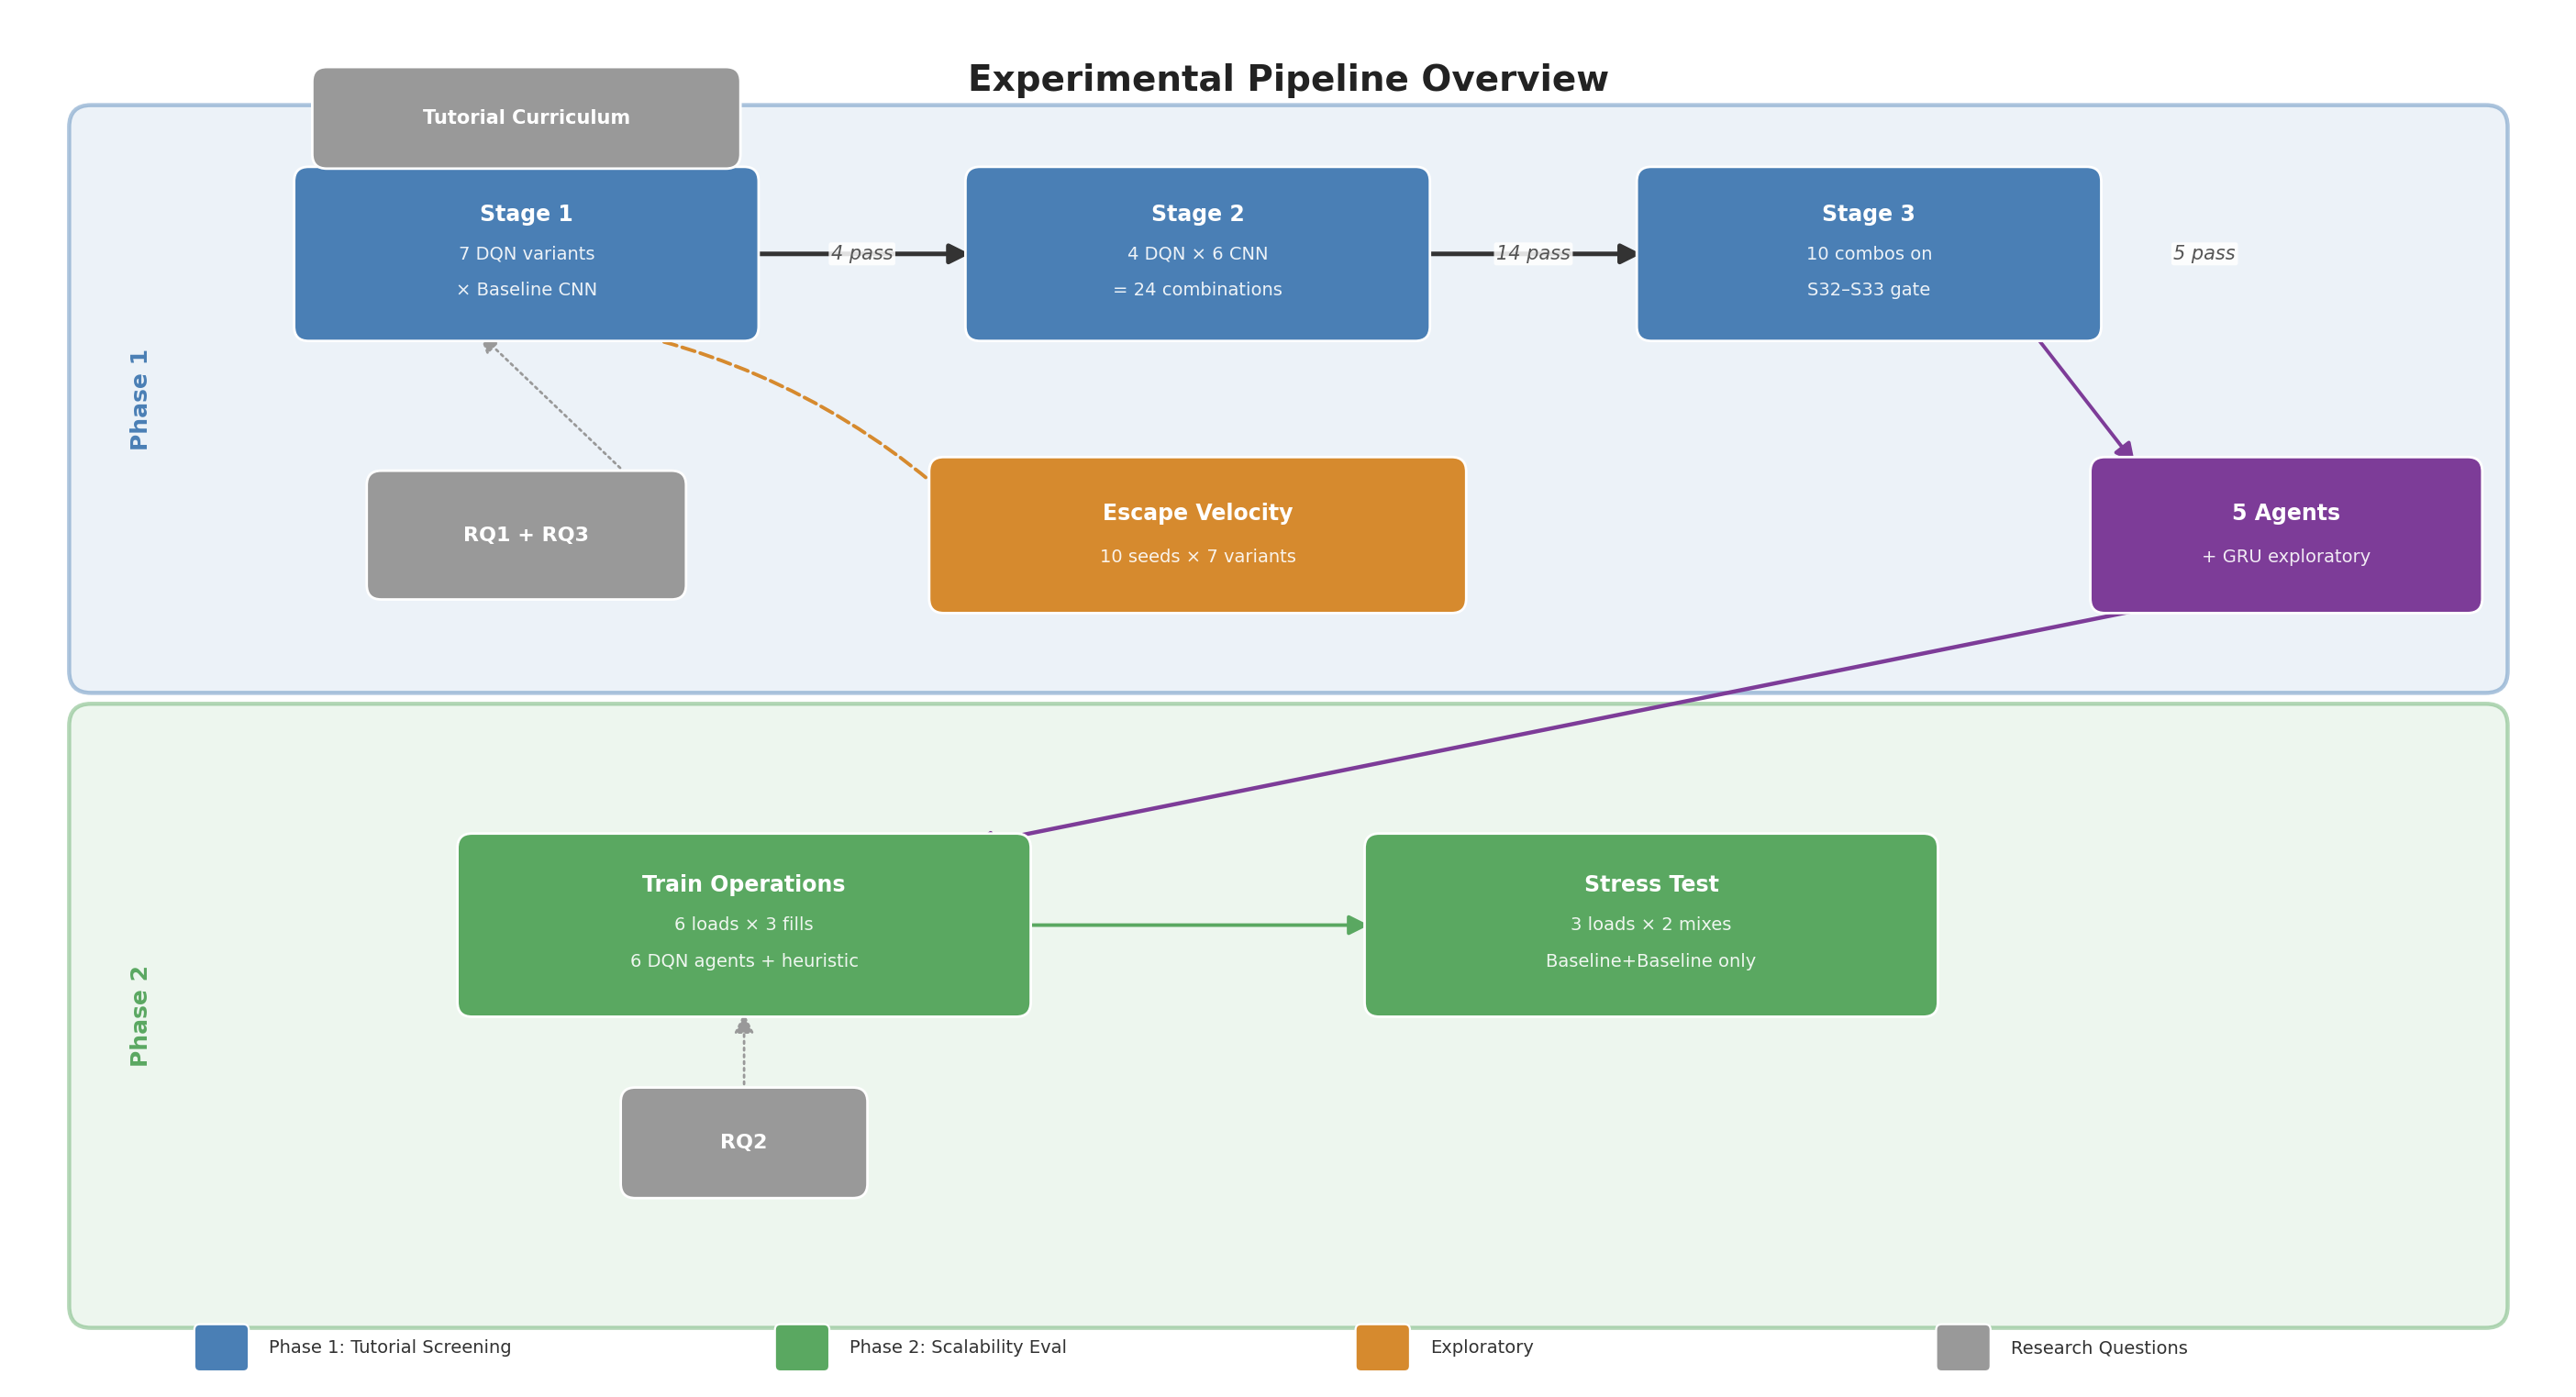
\includegraphics[width=\textwidth]{experimental_overview}
  \caption{Experimental pipeline overview.  Phase~1 progressively narrows 7~DQN variants through three screening stages to 5~confirmed agents.  An escape velocity experiment characterises run-to-run variance.  Phase~2 evaluates scalability on train operations (all 6~agents) and a mixed-operation stress test (Baseline+Baseline only).  Grey boxes indicate which research questions each phase addresses.}
  \label{fig:exp:overview}
\end{figure}

\section{Research Questions and Experimental Rationale}
\label{sec:exp:hypotheses}

The experimental design addresses three research questions.

\textbf{RQ1} (\emph{Can a single DQN-based agent learn the joint problem?}) --- Phase~1 establishes which DQN$\times$CNN combinations master the tutorial suite. Stages~1 and~2 use the 31-scenario, 13-tier curriculum. Stage~3 adds the 14th tier (Operational Readiness, S32--S33) as a final gate.

\textbf{RQ2} (\emph{Do skills scale beyond the training distribution?}) --- Phase~2 evaluates top performers alongside the GRU-augmented variant (\cref{sec:agent:gru}) on controlled scenarios scaling from 40 to 400 containers, testing whether the agent can coordinate all eight container move types at operational scale.

\textbf{RQ3} (\emph{How do individual components contribute?}) --- The factored two-stage design (Stage~1 varies the DQN algorithm with a fixed backbone and Stage~2 varies the backbone with fixed algorithms) isolates each component's marginal contribution and reveals interaction effects.

The full research questions are stated in \cref{sec:intro:rqs}. RQ1 is addressed by the Phase~1 results (\cref{sec:res:phase1}), RQ2 by the Phase~2 evaluation (\cref{sec:res:phase2}), and RQ3 by the cross-combination analysis (\cref{sec:res:phase1:cnn,sec:res:phase1:ranking}).

\section{Architecture Candidates}
\label{sec:exp:architectures}

The architecture search is decomposed into two orthogonal dimensions: the DQN algorithm (the training objective and exploration mechanism) and the CNN backbone (the convolutional feature extractor). Rather than evaluating the full cross-product of all algorithms and all backbones simultaneously, a sequential screening strategy reduces the total number of training runs.

\subsection{Stage 1: DQN Algorithm Screening}
\label{sec:exp:architectures:dqn}

Seven DQN algorithm variants are evaluated, all sharing the same baseline CNN backbone (approximately 141K total parameters). The variants span three families of improvements to the standard Double DQN with Prioritised Experience Replay:

\begin{table}[H]
  \centering
  \caption{DQN algorithm variants evaluated in Stage~1. All variants use the baseline CNN backbone. Parameter counts differ slightly due to variant-specific network heads.}
  \label{tab:exp:dqn_variants}
  \begin{tabularx}{\textwidth}{@{} l l X r @{}}
    \toprule
    \textbf{Variant} & \textbf{Family} & \textbf{Key Modification} & \textbf{Params} \\
    \midrule
    Baseline       & Value-based & Double DQN + PER \cite{hasselt2016ddqn,schaul2016per} & 140{,}834 \\
    Munchausen     & Value-based & Adds scaled log-policy to reward: $r + \alpha \tau \log \policy(a|s)$ \cite{vieillard2020munchausen} & 140{,}834 \\
    Spectral Norm  & Regularisation & Spectral normalisation \cite{miyato2018spectral} on all backbone convolutions & 140{,}834 \\
    NoisyNet       & Exploration  & Parametric noise layers replace $\varepsilon$-greedy \cite{fortunato2018noisy} & 140{,}900 \\
    Dueling        & Architecture & Separate value and advantage streams \cite{wang2016dueling} & 145{,}060 \\
    QR-DQN         & Distributional & Quantile regression with fixed quantile atoms \cite{dabney2018distributional} & 142{,}880 \\
    IQN            & Distributional & Implicit quantile networks with sampled $\tau$ \cite{dabney2018implicit} & 149{,}414 \\
    \bottomrule
  \end{tabularx}
\end{table}

The seven variants cover the major directions in post-DQN algorithmic research: reward augmentation (Munchausen), weight regularisation (Spectral Norm), learned exploration (NoisyNet), architectural decomposition (Dueling), and distributional value estimation (QR-DQN, IQN). Each extension is described in \cref{sec:bg:rl:dqn,sec:rw:dqn}. The table above summarises the key modification and parameter overhead for each variant.

\subsection{Stage 2: CNN Backbone Screening}
\label{sec:exp:architectures:cnn}

Based on the Stage~1 results (presented in \cref{sec:res:phase1:dqn}), the four DQN algorithms that successfully mastered the full tutorial curriculum are selected for the backbone comparison. These are crossed with six CNN backbone variants in a $6 \times 4 = 24$ run grid:

\begin{table}[H]
  \centering
  \caption{CNN backbone variants evaluated in Stage~2. Each backbone is paired with the four top DQN algorithms from Stage~1 (Baseline, Munchausen, Spectral Norm, NoisyNet).}
  \label{tab:exp:cnn_variants}
  \begin{tabularx}{\textwidth}{@{} l X r @{}}
    \toprule
    \textbf{Backbone} & \textbf{Modification} & \textbf{Backbone Params} \\
    \midrule
    Baseline      & 4-layer factored CNN (32$\to$64 channels) as described in \cref{sec:agent:unified:cnn} & ${\sim}108$K \\
    Wider         & Same 4 layers with doubled channel width (64$\to$128 channels) & ${\sim}416$K \\
    Deeper        & 5th convolutional layer (additional cross-region pass) inserted after Stage~2 & ${\sim}145$K \\
    Residual      & Skip connections \cite{he2016resnet} around Stages~2 and~3 & ${\sim}108$K \\
    Narrow-Deep   & Half channel width (16$\to$32), 6 layers total & ${\sim}43$K \\
    Region-Aware  & Separate per-region convolutions before cross-region fusion & ${\sim}120$K \\
    \bottomrule
  \end{tabularx}
\end{table}

\begin{figure}[H]
  \centering
  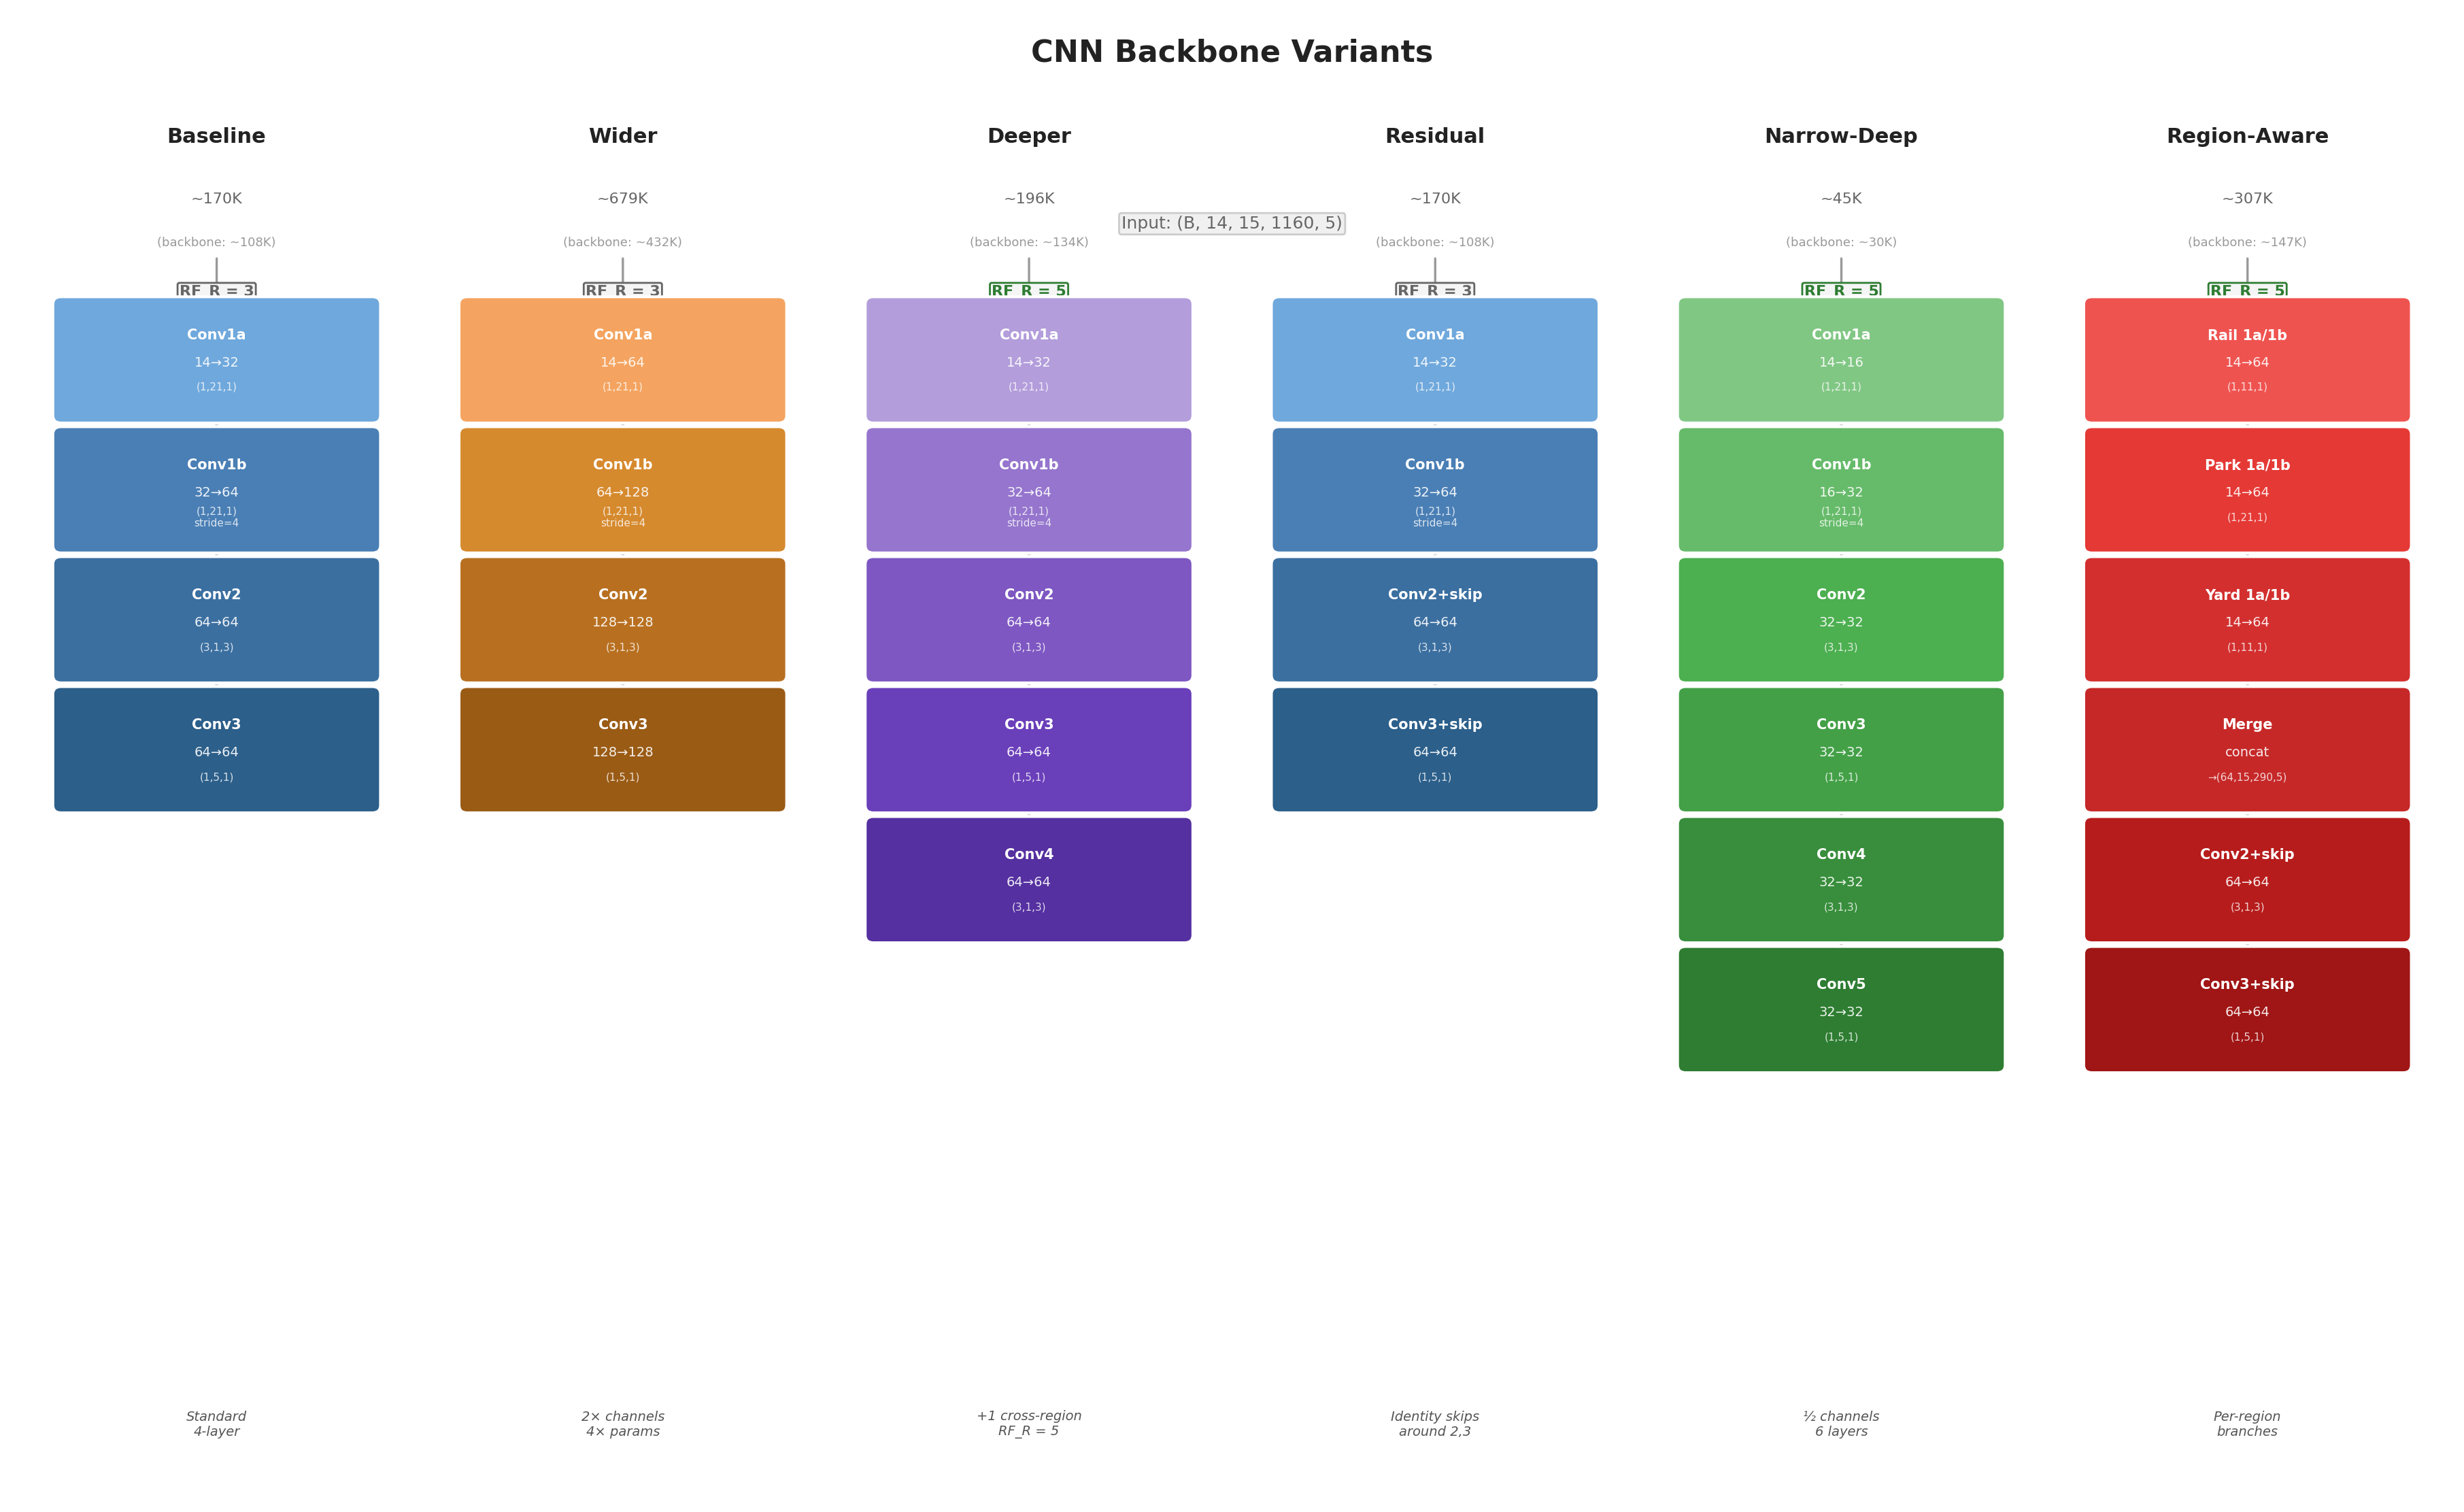
\includegraphics[width=\textwidth]{cnn_backbone_variants}
  \caption{Schematic comparison of the six CNN backbone variants. Each column shows the layer stack, kernel sizes, channel widths, and total parameter count. All variants share the same two-head output structure; only the convolutional feature extractor differs.}
  \label{fig:exp:cnn_variants}
\end{figure}

All backbone variants share the same two-head factored architecture, masking logic, and training hyperparameters. The only differences are CNN depth, channel widths, the presence or absence of skip connections, and structural organisation. The complete hyperparameter specification is listed in \cref{app:hyperparameters}.

\section{Phase 1: Tutorial Screening}
\label{sec:exp:phase1}

\subsection{Protocol}
\label{sec:exp:phase1:protocol}

Each architecture variant is trained through the 31-scenario tutorial curriculum described in \cref{ch:curriculum} with the following fixed parameters:

\begin{itemize}
  \small
  \item \textbf{Random seed:} 42 for all random number generators (Python, NumPy, PyTorch, CUDA).
  \item \textbf{Maximum epochs:} 800. Training terminates early if all 13 tiers are mastered, or if the agent remains stuck at Tier~2 or below after 120 epochs.
  \item \textbf{Mastery threshold:} 90\% pass rate over a rolling window of 20 epochs.
  \item \textbf{Minimum epochs per tier:} 10 before tier advancement is considered.
  \item \textbf{Progress logging:} every 25 epochs for each variant.
\end{itemize}

The two screening stages are executed sequentially. Stage~1 (7 DQN variants $\times$ baseline CNN) is run first. The top-performing algorithms are then paired with all 6 CNN backbones in Stage~2 (24 runs). Each run is executed on a single GPU with aggressive memory cleanup between runs to prevent GPU memory accumulation.

\subsection{Evaluation Metrics}
\label{sec:exp:phase1:metrics}

The primary screening metric is \textbf{epochs to full mastery}: the epoch at which all 13 tiers first achieve $\geq 90\%$ pass rate simultaneously. Variants that exhaust the 800-epoch budget without mastering all tiers are recorded as ``not mastered'' at epoch 800. Variants that fail to progress beyond Tier~2 by epoch 120 are early-stopped to conserve GPU time.

Secondary metrics include the average pass rate (mean per-scenario pass rate at the final epoch over all 31 scenarios), the highest tier reached, wall-clock training time, and per-scenario pass rates for failure mode diagnosis. Scenarios in tiers that were never unlocked receive a 0\% pass rate.

\subsection{Selection Criteria}
\label{sec:exp:phase1:selection}

For Stage~1, an algorithm is selected for Stage~2 if and only if it achieves full mastery within the 800-epoch budget. This binary criterion reflects the observation from \cref{sec:curr:screening} that algorithms unable to master the tutorial suite are unlikely to produce useful policies at scale.

For Stage~2, the final ranking considers both epoch-to-mastery count and average pass rate. Among variants that achieve full mastery, faster convergence is preferred. Among variants with similar convergence speed, higher final pass rates indicate more robust learning.

\subsection{Run-to-Run Variability}
\label{sec:exp:phase1:variability}

Although all random seeds are fixed at 42, run-to-run variance arises from both stochastic scenario elements (randomised container sizes and distractor placements in Tier~4 and above) and GPU non-determinism (see \cref{sec:exp:reproducibility}). The Baseline CNN $\times$ Baseline DQN combination, for instance, mastered the curriculum at epoch 320 in Stage~1 and at epoch 310 in Stage~2, a difference of approximately 3\%. This variability is inherent to the training process and should be kept in mind when interpreting small differences between configurations. The ranking is therefore based on consistent patterns across multiple comparisons rather than single-number differences. A dedicated multi-seed escape velocity experiment (\cref{sec:res:variance}) quantifies this variability and reveals that single-seed screening can produce false negatives for algorithms that succeed stochastically but not reliably.

\section{Phase 2: Controlled Scalability Evaluation}
\label{sec:exp:phase2}

Phase~2 takes the highest-scoring CNN$\times$DQN combinations from the tutorial screening and evaluates their ability to handle container loads far exceeding the training distribution. The tutorials establish that these architectures can learn the component spatial skills on scenarios with at most ${\sim}30$ containers. Phase~2 tests whether these skills generalise to 40--400 containers, with controlled variation of imports, exports, yard fill, and truck operations.

\subsection{From Full Simulation to Controlled Scenarios}
\label{sec:exp:phase2:rationale}

The original experimental plan envisaged three consecutive phases: Phase~0 would screen DQN algorithm variants on tutorials, Phase~1 would cross the survivors with CNN backbones, and Phase~2 would evaluate the final agent in the full stochastic simulation (a multi-day environment with KDE-based vehicle arrivals, dynamic truck queuing, and multi-day carryover effects).

During development, this linear plan proved impractical. The full simulation's logistics chains contain cascading dependencies: a parking bug silently blocks all subsequent truck unloads, a resolver mismatch prevents any yard-to-truck delivery, and a sequential crane timing error makes feasible departure windows appear physically impossible (\cref{sec:disc:engineering}). In the stochastic environment, these bugs were indistinguishable from agent limitations. When an agent fails to export 50\% of scheduled containers, the failure could reflect insufficient capability, an unlucky arrival pattern, a simulation defect, or a reward design flaw. Days of troubleshooting in the full simulation yielded ambiguous results. The same bugs became immediately visible once the \texttt{ScalableEvalScenario} class was built. The class enabled controlled scenarios with known expected outcomes, deterministic initial conditions, and independently variable parameters.

Three properties make controlled scenarios the stronger evaluation methodology.

\textbf{Confounding variables.} The full simulation couples stochastic arrival timing, yard carryover state, concurrent train conflicts, and reward dynamics into a single observation. The controlled scenarios isolate each factor, making it possible to attribute performance changes to specific causes.

\textbf{Reproducibility.} The KDE-based arrival model produces different vehicle schedules on each run because the kernel density estimate is sensitive to the resampling order. The controlled scenarios use deterministic container placement and physics-based departure windows, producing identical initial conditions across runs.

\textbf{Parameter isolation.} The full simulation varies all factors simultaneously: more containers per day means more trains, more trucks, more concurrent operations, and higher yard congestion. The controlled evaluation grid independently varies imports, exports, yard fill percentage, and truck operations, revealing which specific parameter combination causes degradation.

The controlled scenarios therefore serve as the primary scalability evaluation. They answer the core question --- ``can the agent handle $N$ containers at fill level $F\%$?'' --- with high signal-to-noise ratio. What they do not test is sustained multi-day performance with carryover effects, stochastic arrival handling, and yard congestion buildup over time. These aspects --- which relate primarily to the pre-marshalling and long-horizon planning capabilities that the memoryless architecture is structurally unable to provide (\cref{sec:disc:interpretation:scalability}) --- remain directions for future work with temporal architectures.

\subsection{Scalable Evaluation Scenarios}
\label{sec:exp:phase2:scenarios}

The evaluation uses a parameterised scenario system (\texttt{ScalableEvalScenario}) that generates terminal configurations from a small set of parameters: number of imports, exports, delivery trucks, pickup trucks, direct transfers, and yard fill percentage. Each scenario is a self-contained episode that proceeds as follows:

\begin{enumerate}
  \small
  \item \textbf{Yard fill.} If \texttt{yard\_fill\_pct} $> 0$, distractor containers are placed in the yard to simulate a partially filled terminal. These are inert containers that are not assigned to any vehicle but may need to be reshuffled to access target containers beneath them.
  \item \textbf{Export containers.} Export containers are placed in the yard at positions determined by \texttt{find\_single\_placement}, which validates bounds, occupancy, and goods-zone constraints for all seven container sizes (20ft--45ft). Each export is assigned to a departing train.
  \item \textbf{Import trains.} Trains are created with import containers loaded into wagons, distributed across rail tracks. The number of trains is computed from the container count and wagon capacity (${\sim}1.5$ containers per wagon for mixed sizes).
  \item \textbf{Trucks.} Delivery trucks carry containers to be unloaded into the yard. Pickup trucks arrive to collect specific import containers. Direct-transfer containers (train-to-truck, truck-to-train) exercise cross-modal paths.
  \item \textbf{Departure window.} A physics-based timing model computes the minimum feasible time for all required crane moves, accounting for trapezoidal motion profiles (gantry, trolley, hoist), parallel crane execution, and a configurable safety factor for agent inefficiency. Train departures are scheduled at this computed time, ensuring the scenario is physically feasible but not overly generous.
\end{enumerate}

Success requires completing all scheduled operations before train departure: all imports unloaded to yard, all exports loaded onto trains, all trucks served. The scenario reports granular sub-task progress (imports done, exports done, trucks served) for diagnostic analysis.

\subsection{Evaluation Grid}
\label{sec:exp:phase2:grid}

The primary evaluation matrix varies the total container load across six levels and crosses each with three yard fill percentages:

\begin{table}[H]
  \centering
  \caption{Primary evaluation grid: container loads $\times$ yard fill levels.  Imports and exports are split evenly (e.g., 200 total $=$ 100 imports $+$ 100 exports).  Each cell is run across 30~warmup epochs with cumulative training.}
  \label{tab:exp:eval_grid}
  \begin{tabular}{@{} l r r r r r r @{}}
    \toprule
    \textbf{Fill \textbackslash{} Total} & \textbf{40} & \textbf{80} & \textbf{120} & \textbf{200} & \textbf{300} & \textbf{400} \\
    \midrule
    0\%   & \checkmark & \checkmark & \checkmark & \checkmark & \checkmark & \checkmark \\
    25\%  & \checkmark & \checkmark & \checkmark & \checkmark & \checkmark & \checkmark \\
    50\%  & \checkmark & \checkmark & \checkmark & \checkmark & \checkmark & \checkmark \\
    \bottomrule
  \end{tabular}
\end{table}

This yields 18 parameter combinations per agent, each run for 30~warmup epochs, producing 540~evaluation episodes per agent.  The primary grid tests \textbf{train operations only}: imports (TRAIN\_TO\_YARD) and exports (YARD\_TO\_TRAIN), with yard reshuffles (YARD\_TO\_YARD) as needed.  Truck operations (PARK\_TRUCK, TRUCK\_TO\_YARD, YARD\_TO\_TRUCK) and direct transfers (TRAIN\_TO\_TRUCK, TRUCK\_TO\_TRAIN) are reserved for a secondary mixed-operation stress test (\cref{sec:res:phase2:stress}), run on the Baseline+Baseline agent to establish whether the simplest DQN architecture can coordinate all eight move types at scale.

\subsection{Agent Selection}
\label{sec:exp:phase2:selection}

Rather than committing to a single agent, Phase~2 evaluates the five CNN$\times$DQN combinations that passed the Stage~3 operational-readiness gate (\cref{sec:res:phase1:stage3}), plus one additional exploratory variant:

\begin{enumerate}
  \item \textbf{Baseline + Baseline} (Stage~3 rank~5, 310 epochs, 98.6\%)
  \item \textbf{Baseline + Narrow-Deep} (Stage~3 rank~1, 293 epochs, 99.2\%)
  \item \textbf{NoisyNet + Narrow-Deep} (Stage~3 rank~10, 349 epochs, 99.4\%)
  \item \textbf{Spectral Norm + Deeper} (Stage~3 rank~3, 305 epochs, 99.2\%)
  \item \textbf{Munchausen + Baseline} (Stage~3 rank~7, 319 epochs, 98.6\%)
  \item \textbf{GRU-DQN + Narrow-Deep} (exploratory --- not in Phase~1).  This recurrent variant, described in \cref{sec:agent:gru}, augments the feedforward path with a GRU cell that maintains a persistent hidden state across decision steps within an episode, adding approximately 45.8K parameters (32\% overhead).  The GRU variant was developed between Phase~1 and Phase~2 as one of two exploratory temporal extensions (alongside an LSTM burn-in approach inspired by R2D2 \cite{kapturowski2019r2d2}) to probe whether temporal context improves scalability.  Neither temporal variant was included in Phase~1 screening. The GRU is included in Phase~2 as an exploratory probe independent of the Phase~1 ranking.
\end{enumerate}

Evaluating multiple agents allows a direct comparison of how different training algorithms and backbone architectures scale to loads far beyond the tutorial distribution, rather than relying on a single agent's performance.  A priority-based \textbf{heuristic baseline} provides a non-learned reference point (\cref{sec:exp:phase2:baselines}).

\subsection{Evaluation Protocol}
\label{sec:exp:phase2:config}

The evaluation uses the same terminal geometry as Phase~1 (5 yard rows $\times$ 58 bays $\times$ 5 tiers, 7 rail tracks, split factor 20).  Each agent processes the 18~parameter combinations sequentially.  For each combination, the agent runs 30~warmup episodes with $\varepsilon = 0.10$ exploration and 4~gradient steps per episode, recording per-epoch metrics.  Training is cumulative across combinations --- weights and replay buffer carry over --- allowing the agent to adapt progressively to increasing scenario scale.  The final warmup epoch (epoch~29) serves as the measured evaluation for that combination.

This cumulative protocol is a deliberate extension of the curriculum learning philosophy into the evaluation phase.  The tutorials provide a strong weight initialisation; the warmup episodes are the next curriculum stage, where the agent encounters operational-scale workloads for the first time and adapts its policy online.  This mirrors a realistic deployment scenario: a terminal operator would train an agent on tutorials, then deploy it on real workloads while allowing continued learning.  The agent faces a \emph{continuous} problem. This means that workload characteristics shift as container counts, fill levels, and traffic patterns change. This makes online adaptation a core reinforcement learning capability rather than a methodological artefact.  Freezing weights after tutorials and evaluating zero-shot performance would test memorisation. Cumulative training tests the agent's ability to \emph{generalise and adapt}, which is the more operationally relevant question.

\subsection{Evaluation Metrics}
\label{sec:exp:phase2:metrics}

Each scenario run produces:

\begin{enumerate}
  \small  
  \item \textbf{Pass/Fail:} Binary outcome --- did the agent complete all scheduled operations before train departure?
  \item \textbf{Sub-task progress:} Fraction of imports unloaded, exports loaded, and trucks served. A scenario may fail overall but achieve 90\% of imports, pinpointing the bottleneck.
  \item \textbf{Move counts:} Per-move-type tallies (TRAIN\_TO\_YARD, YARD\_TO\_TRAIN, PARK\_TRUCK, etc.) reveal the agent's operational strategy.
  \item \textbf{Total reward:} Accumulated reward validates that the reward function scales sensibly with container count.
\end{enumerate}

\subsection{Baselines}
\label{sec:exp:phase2:baselines}

A priority-based \textbf{heuristic agent} provides a non-learned reference.  The heuristic evaluates sources in a fixed priority order --- (1)~YARD\_TO\_TRAIN, (2)~TRAIN\_TO\_YARD, (3)~PARK\_TRUCK, (4)~TRUCK\_TO\_YARD, (5)~YARD\_TO\_TRUCK, (6)~YARD\_TO\_YARD --- and for each priority level scans the source mask deterministically, selecting the first valid source--destination pair.  It uses no exploration, no replay buffer, and no gradient updates.  This provides a lower-bound reference: performance that a hand-coded dispatcher achieves without any learning.

Additionally, the evaluation grid itself serves as an internal baseline: each agent's performance is compared across parameter combinations to identify the container count and yard fill level at which performance degrades.

\section{Hardware and Software Environment}
\label{sec:exp:hardware}

All experiments were conducted on a workstation with an NVIDIA GeForce RTX 2060 Super GPU (8\,GB VRAM), running Ubuntu under WSL2. The software environment uses Python~3.12, PyTorch~2.10 with CUDA~12.8, and scikit-learn~1.8. The Stage~1 DQN screening (7 runs) completed in approximately 3.5 hours of wall-clock time. The Stage~2 CNN$\times$DQN grid (24 runs) required approximately 22 hours. All training was performed in Jupyter notebooks with automated logging for reproducibility.

\section{Reproducibility}
\label{sec:exp:reproducibility}

All random seeds are fixed at 42 across Python, NumPy, PyTorch, and CUDA backends. The tutorial scenario definitions, hyperparameter configurations, and agent factory functions are version-controlled in the project repository. Training logs are parsed into structured JSON results files that can be reloaded to reproduce all figures and tables in \cref{ch:results} without re-running the training.

\paragraph{GPU non-determinism.}
Run-to-run variance was observed even with identical random seeds. This is attributable to non-deterministic CUDA operations --- in particular, atomic floating-point reductions (\texttt{atomicAdd}) in the \texttt{Conv3d} backward passes, where the parallel summation order varies between runs, producing different rounding errors that compound over training \cite{pytorch_reproducibility}. Additional non-determinism arises from cuDNN's benchmark mode, which selects the fastest convolution algorithm at runtime; timing noise can cause a different algorithm to be selected on each run, producing numerically different feature maps. PyTorch provides determinism flags (\texttt{torch.backends.cudnn.deterministic}, \texttt{torch.use\_deterministic\_algorithms}) that suppress these sources, but at a 10--30\% training time penalty and with incomplete coverage of all operations. Rather than imposing this overhead, we characterise the variance empirically through the escape velocity experiment (\cref{sec:res:variance:escape}) and report distributional results where relevant. As shown in that section, the variance is itself informative: it reveals that cross-region primitive acquisition acts as a stochastic bifurcation point in the optimisation landscape, separating stochastic seed-dependent failure from systematic architectural failure.

% chapters/09_results.tex
\chapter{Results}
\label{ch:results}

This chapter presents the results of both evaluation phases described in \cref{ch:experiments}. \Cref{sec:res:phase1} reports the three-stage tutorial screening (RQ1, RQ3), including a multi-seed escape velocity experiment that distinguishes systematic from stochastic architectural failures. \Cref{sec:res:phase2} reports the controlled scalability evaluation (RQ2).

% ====================================================================
\section{Phase 1: Tutorial Screening Results}
\label{sec:res:phase1}
% ====================================================================

Phase~1 answers RQ1 and RQ3 simultaneously: the three-stage screening reveals which architectures can learn the joint terminal coordination problem, and the factored design isolates each component's contribution.

\subsection{Stage 1: DQN Algorithm Comparison}
\label{sec:res:phase1:dqn}

Seven DQN algorithm variants were trained on the tutorial curriculum using the baseline CNN backbone. \Cref{tab:res:dqn_summary} summarises the outcome of each run.

\begin{table}[H]
  \centering
  \caption{Stage~1 results: DQN algorithm variants ranked by epochs to mastery. All variants use the baseline CNN backbone (${\sim}141$K parameters). ``Tier'' indicates the highest tier mastered within the 800-epoch budget. Variants that failed to progress beyond Tier~2 by epoch 120 were early-stopped.}
  \label{tab:res:dqn_summary}
  \begin{tabular}{@{} l r l r r r @{}}
    \toprule
    \textbf{Variant} & \textbf{Epochs} & \textbf{Mastered} & \textbf{Tier} & \textbf{Avg Rate} & \textbf{Wall (s)} \\
    \midrule
    Munchausen     & 317 & Yes & 13/13 & 97.7\% & 1{,}649 \\
    Baseline       & 320 & Yes & 13/13 & 98.9\% & 1{,}561 \\
    Spectral Norm  & 343 & Yes & 13/13 & 99.2\% & 1{,}627 \\
    NoisyNet       & 522 & Yes & 13/13 & 97.4\% & 6{,}877 \\
    \midrule
    Dueling        & 120 & No  & 0/13  & 8.4\%  & 624 \\
    QR-DQN         & 120 & No  & 0/13  & 9.7\%  & 596 \\
    IQN            & 120 & No  & 0/13  & 9.7\%  & 758 \\
    \bottomrule
  \end{tabular}
\end{table}

The results (\cref{tab:res:dqn_summary,fig:res:dqn_epochs}) show an apparent binary outcome: four variants achieve full mastery while three are early-stopped at Tier~0. The top three (Munchausen, Baseline, Spectral Norm) form a tight cluster within 26 epochs of each other, while NoisyNet is a clear outlier at 522 epochs --- indicating substantial sensitivity to the training algorithm even with identical network architecture. However, the escape velocity experiment (\cref{sec:res:variance:escape}) reveals that this binary classification is incomplete: IQN escapes Tier~0 in 9 of 10 multi-seed runs and QR-DQN in 2 of 10, so their single-seed failures were at least partially stochastic. Only Dueling fails on all 10 seeds.

\begin{figure}[H]
  \centering
  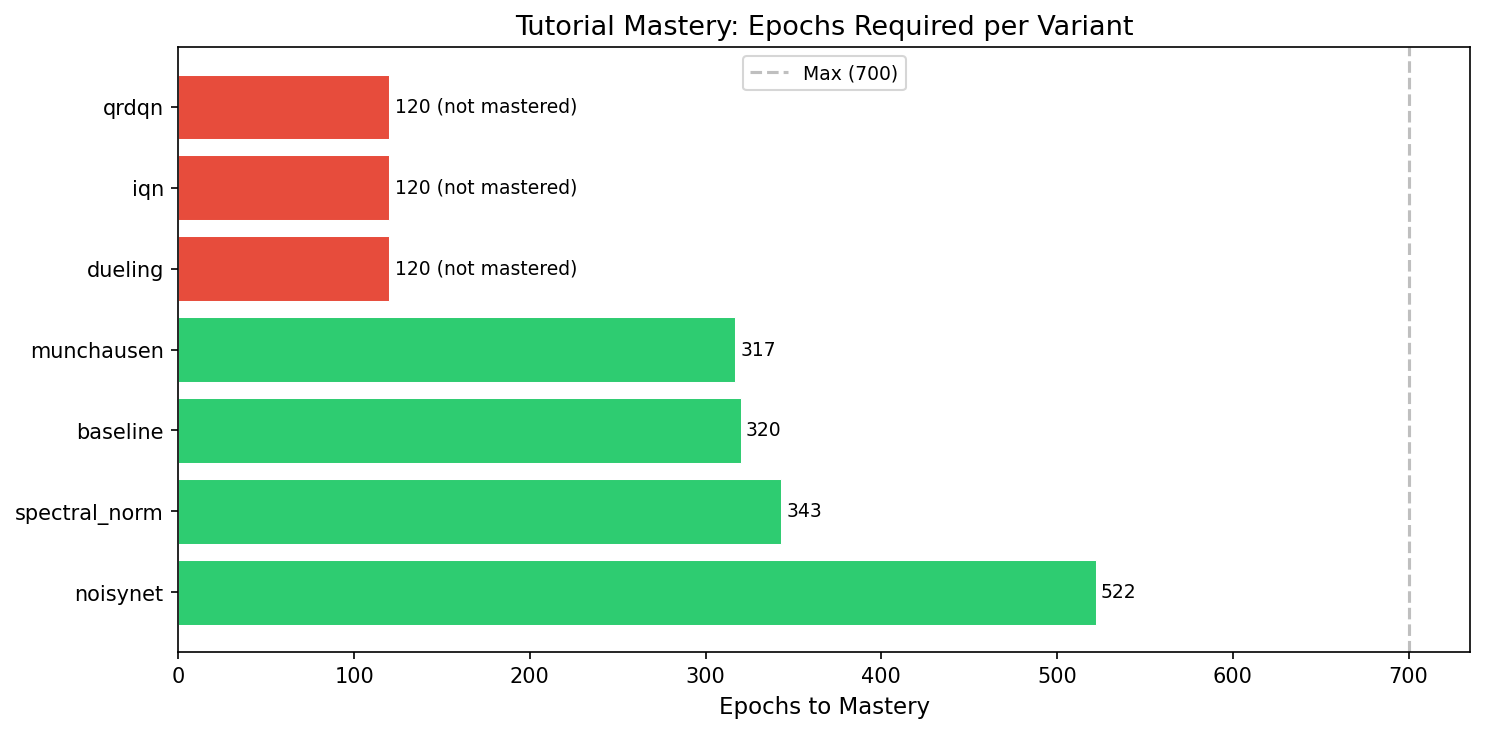
\includegraphics[width=0.85\textwidth]{variant_epochs}
  \caption{Epochs to mastery for all seven DQN algorithm variants. Green bars indicate full mastery; red bars indicate early-stopped variants that failed to progress beyond Tier~2 by epoch 120. Munchausen achieves the fastest convergence at 317 epochs.}
  \label{fig:res:dqn_epochs}
\end{figure}

\subsubsection{Per-Scenario Analysis}

\Cref{fig:res:dqn_heatmap} shows the per-scenario pass rates. The four successful variants achieve near-perfect scores across all tiers; the primary differentiator is S21 (\texttt{full\_mini\_day}), which requires all logistics skills simultaneously and drops to 70\% for both Munchausen and NoisyNet. On the single seed, all three failed variants stall at S4 (\texttt{yard\_to\_train}), suggesting a uniform cross-region failure --- but the escape velocity data (\cref{sec:res:variance:escape}) reveals that each variant fails on a \emph{different} primitive: Dueling on S3, QR-DQN on S4, and IQN only occasionally on S4.

\begin{figure}[H]
  \centering
  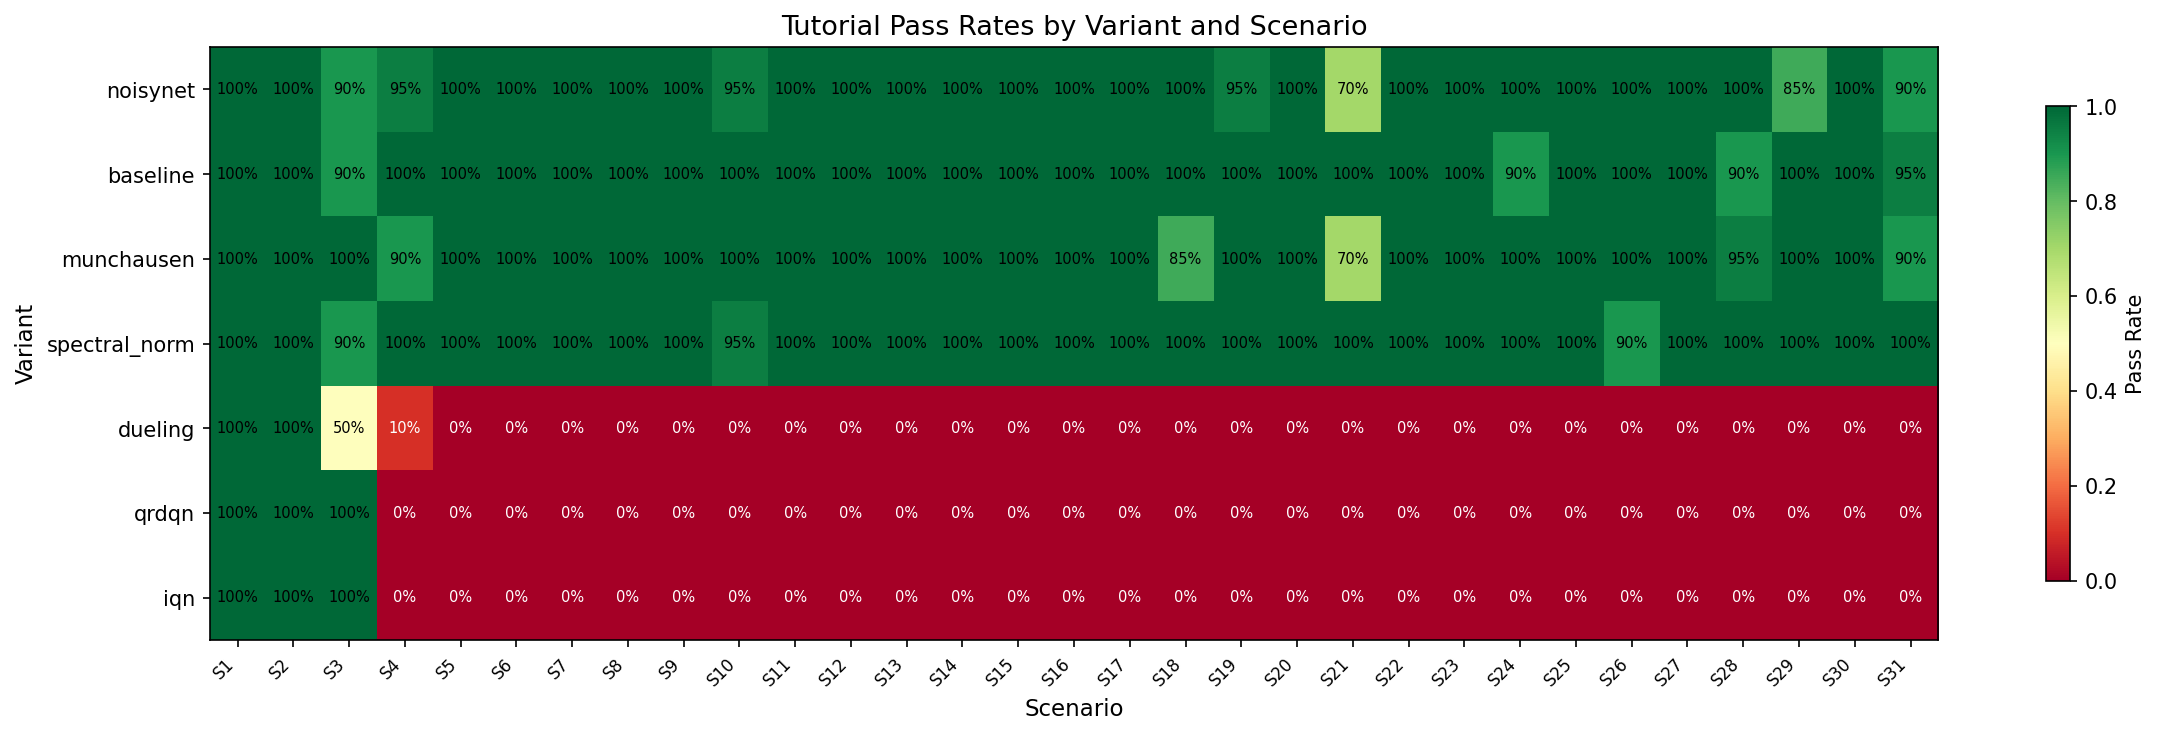
\includegraphics[width=\textwidth]{variant_heatmap}
  \caption{Per-scenario pass rates for all seven DQN variants. Rows represent variants (ordered by convergence speed); columns represent the 31 tutorial scenarios (S1--S31). Green indicates high pass rates; red indicates failure. The three unsuccessful variants all stall at S4 (\texttt{yard\_to\_train}).}
  \label{fig:res:dqn_heatmap}
\end{figure}

\subsubsection{Selection for Stage 2}

All four successful variants are selected for Stage~2, following the binary mastery criterion from \cref{sec:exp:phase1:selection}.

% ────────────────────────────────────────────────────────────────
\subsection{Variance Estimation: Escape Velocity}
\label{sec:res:variance}

Before proceeding to the backbone comparison, we address the single-seed limitation of Stage~1 using the escape velocity protocol described in \cref{sec:exp:phase1:variability}: each of the seven DQN variants is trained for 100~epochs on Tier~0 only (S1--S4) across 10~replicate runs, with variance arising solely from GPU non-determinism (\cref{sec:exp:reproducibility}).

\begin{table}[H]
  \centering
  \caption{Escape velocity results: 10-run Tier~0 escape rates per DQN variant. Each run trains for 100 epochs on the four primitive scenarios (S1--S4) with the baseline CNN backbone. All runs use seed~42; variance arises from GPU non-determinism. ``S3'' and ``S4'' columns report median pass rate with [min--max] range across the 10 runs.}
  \label{tab:res:escape_rates}
  \begin{tabular}{@{} l r r r r @{}}
    \toprule
    \textbf{Variant} & \textbf{Escaped} & \textbf{Escape Rate} & \textbf{S3 (\%)} & \textbf{S4 (\%)} \\
    \midrule
    Baseline       & 10/10 & 100\% & 90 [90--90] & 98 [95--100] \\
    Munchausen     & 10/10 & 100\% & 90 [90--100] & 98 [90--100] \\
    Spectral Norm  & 10/10 & 100\% & 90 [90--100] & 95 [90--100] \\
    NoisyNet       & 10/10 & 100\% & 90 [90--100] & 95 [90--100] \\
    \midrule
    IQN            &  9/10 &  90\% & 100 [90--100] & 90 [30--100] \\
    QR-DQN         &  2/10 &  20\% & 50 [0--100] & 0 [0--90] \\
    Dueling        &  0/10 &   0\% & 35 [0--85] & 93 [15--100] \\
    \bottomrule
  \end{tabular}
\end{table}

\begin{figure}[H]
  \centering
  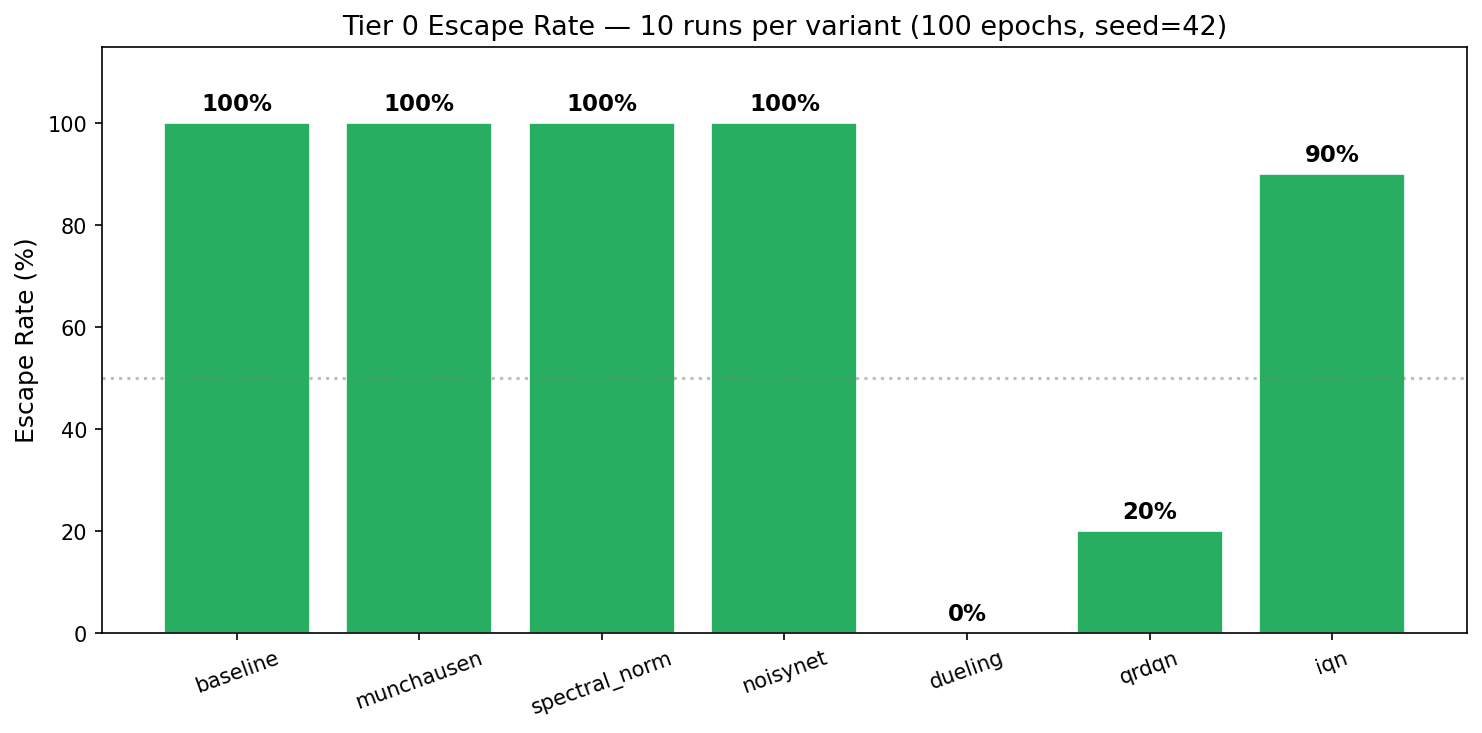
\includegraphics[width=0.85\textwidth]{escape_velocity_rates}
  \caption{Tier~0 escape rates across 10 runs per DQN variant. The four robust variants (Baseline, Munchausen, Spectral Norm, NoisyNet) achieve 100\% escape. IQN escapes in 90\% of runs, QR-DQN in 20\%, and Dueling never escapes.}
  \label{fig:res:escape_rates}
\end{figure}

\subsubsection{The Primitives Gateway}
\label{sec:res:variance:escape}

The results in \cref{tab:res:escape_rates} reveal a more nuanced picture than the binary pass/fail classification suggested by the single-seed screening. The seven DQN variants separate into three tiers of reliability:

\begin{enumerate}
  \item \textbf{Robust} (100\% escape): Baseline, Munchausen, Spectral Norm, and NoisyNet escape Tier~0 in all 10 runs with tight ranges (S3 and S4 both $\geq 90\%$ on every run). These algorithms reliably learn cross-region spatial coordination within 100 epochs regardless of GPU non-determinism.

  \item \textbf{Fragile} (20--90\% escape): IQN and QR-DQN can learn the cross-region primitives but fail stochastically. IQN is surprisingly strong: it achieves a median of 100\% on S3 (\texttt{yard\_to\_truck}) but occasionally drops S4 (\texttt{yard\_to\_train}) to 30\%, causing 1-in-10 escape failure. QR-DQN is bimodal on S3 (individual runs either achieve 100\% or 0\%) and consistently weak on S4 (median 0\%, range 0--90\%), escaping only 2 of 10 times.

  \item \textbf{Incompatible} (0\% escape): Dueling never escapes on any run. Its bottleneck is S3 (\texttt{yard\_to\_truck}, median 35\%, range 0--85\%) rather than S4, which it partially learns (median 93\%). The advantage decomposition $Q(s,a) = V(s) + A(s,a) - \overline{A}$ is structurally incompatible with the high-dimensional spatial action space: the mean-advantage subtraction over ${\sim}21{,}750$ spatial positions (most masked to $-\infty$) disrupts the fine-grained positional discrimination needed for cross-region moves.
\end{enumerate}

\begin{figure}[H]
  \centering
  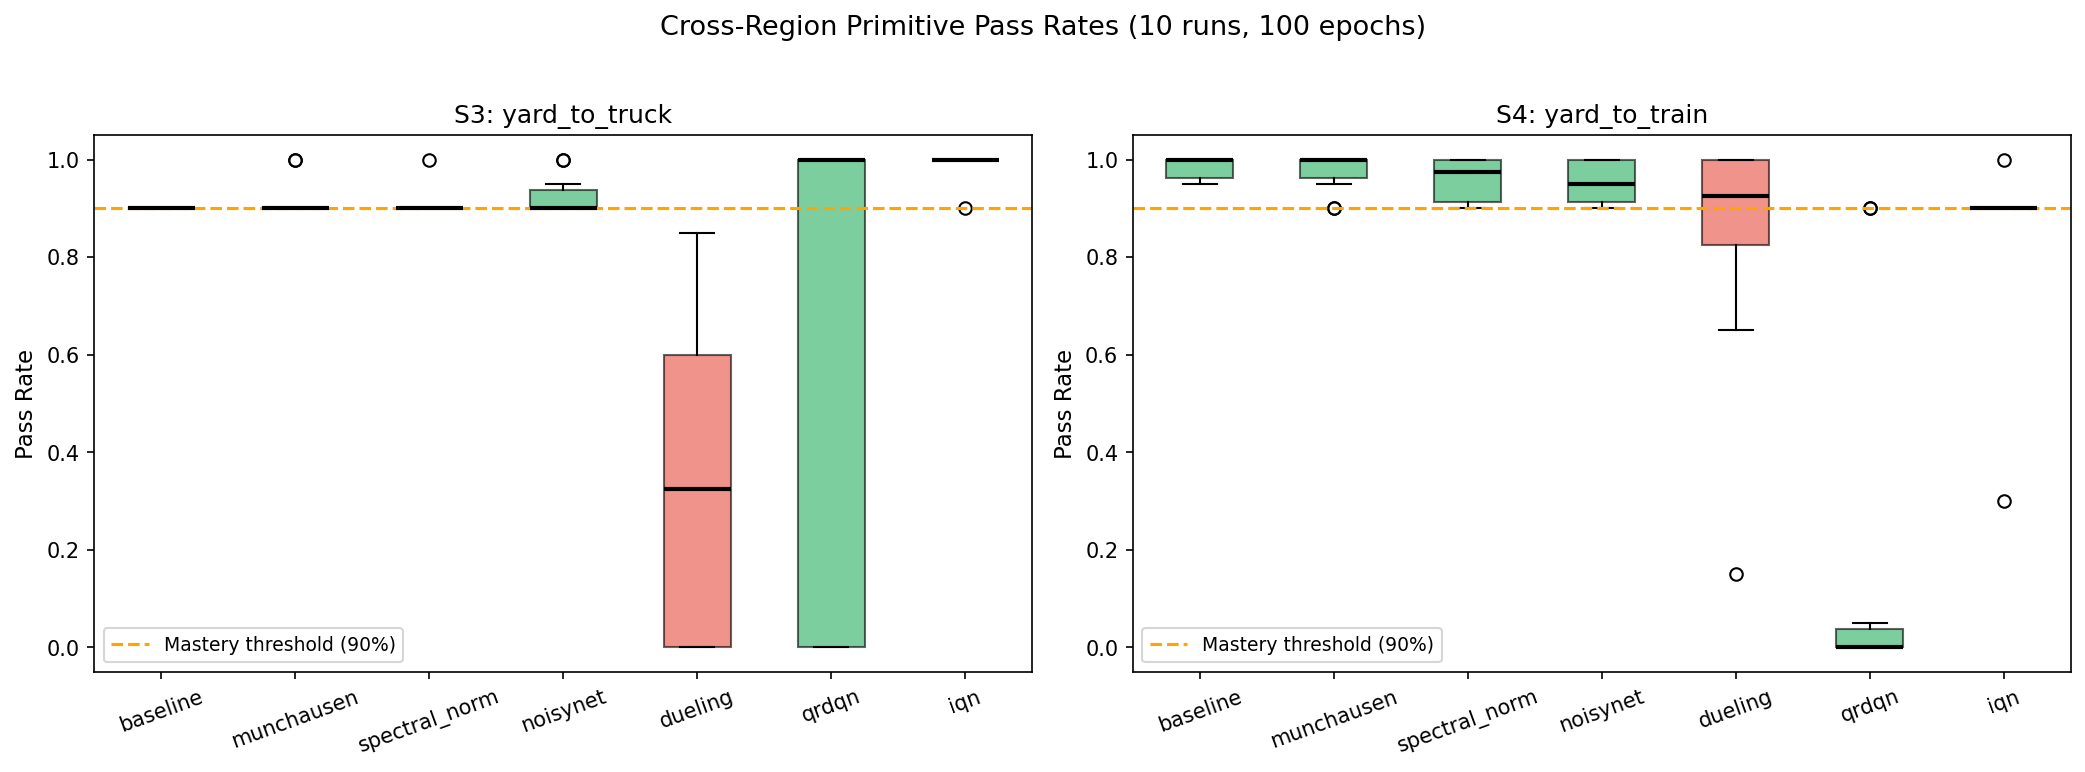
\includegraphics[width=\textwidth]{escape_velocity_s3_s4_boxplot}
  \caption{Distribution of cross-region primitive pass rates across 10 runs per variant. Green boxes indicate variants that escape at least once; red indicates Dueling (0\% escape). The orange dashed line marks the 90\% mastery threshold. The boxplots reveal that each failing variant has a \emph{different} bottleneck: Dueling on S3, QR-DQN on S4, and IQN occasionally on S4.}
  \label{fig:res:s3s4_boxplot}
\end{figure}

\begin{figure}[H]
  \centering
  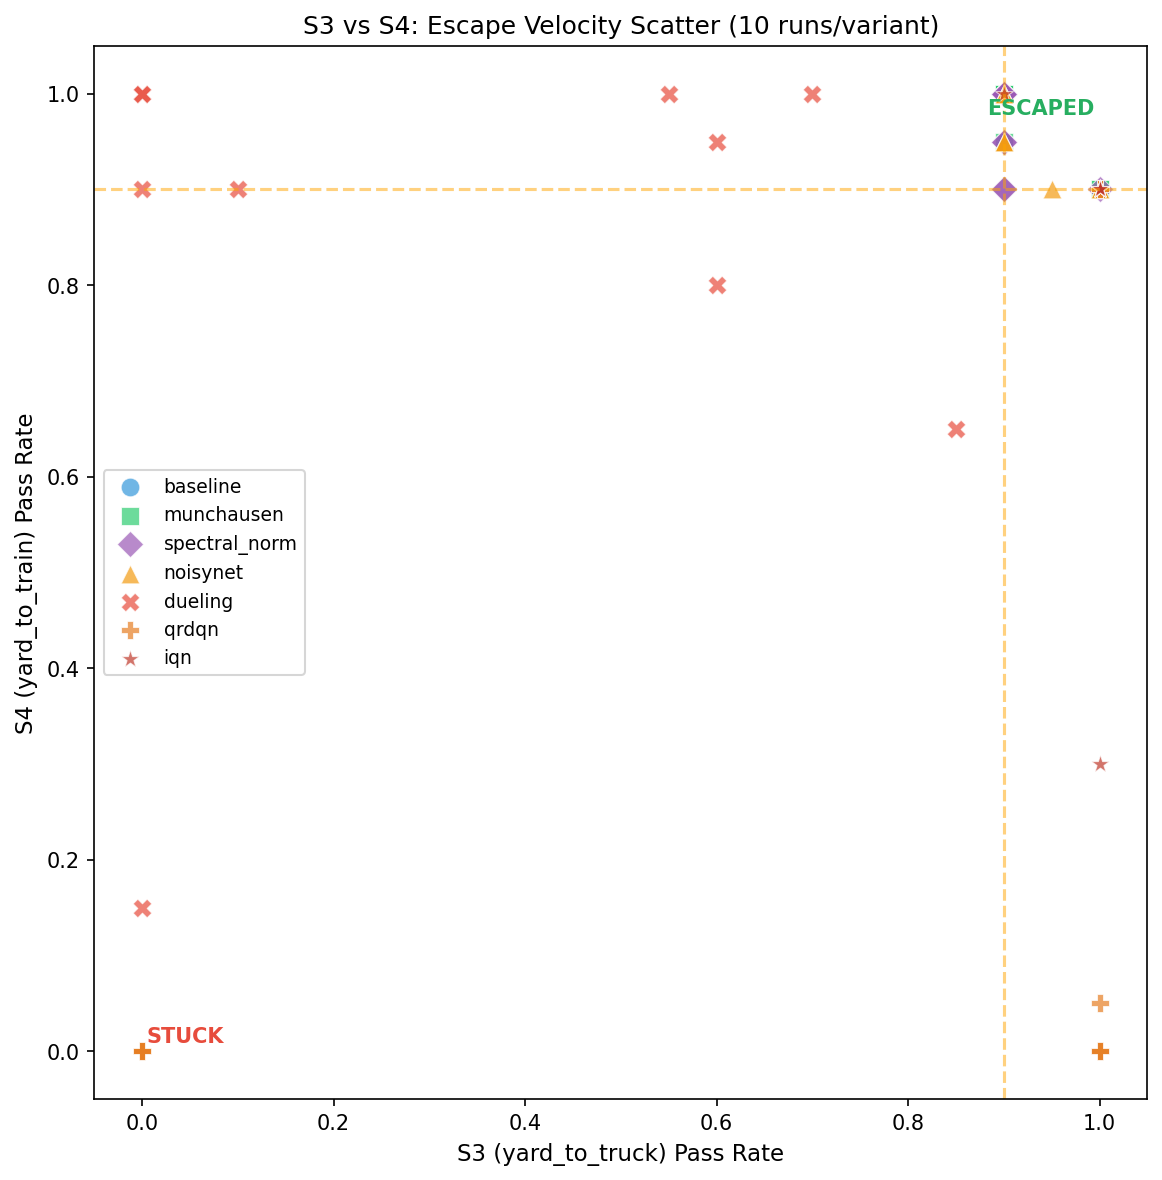
\includegraphics[width=0.75\textwidth]{escape_velocity_scatter}
  \caption{Each point represents one training run, plotted by its S3 (\texttt{yard\_to\_truck}) and S4 (\texttt{yard\_to\_train}) pass rates. The orange dashed lines mark the 90\% mastery threshold. Runs in the upper-right quadrant escaped Tier~0; those outside did not. The four robust variants form a tight cluster. The fragile and incompatible variants scatter along different failure axes.}
  \label{fig:res:s3s4_scatter}
\end{figure}

\Cref{fig:res:s3s4_boxplot} shows the per-scenario pass rate distributions, and \cref{fig:res:s3s4_scatter} plots each run as a point in $(\text{S3}, \text{S4})$ space. The scatter plot is particularly revealing: the four robust variants cluster tightly in the upper-right ``escaped'' quadrant, while the fragile and incompatible variants scatter across the plot, each failing in a distinct direction.

A critical finding is that S3 and S4 test \emph{different} cross-region spatial mappings, and variants fail on different ones:

\begin{itemize}
  \item \textbf{Dueling} fails primarily on S3 (yard$\to$truck, median 35\%) but partially learns S4 (yard$\to$train, median 93\%). The truck parking region (row~7) is a single row sandwiched between rail (rows~0--6) and yard (rows~8--12), making it the hardest destination for the advantage stream to discriminate.
  \item \textbf{QR-DQN} is bimodal on S3 (individual runs either 0\% or 100\%) and catastrophically fails on S4 (median 0\%). The 32-quantile output head produces $32 \times 21{,}750$ values per forward pass, overwhelming the spatial gradient signal for the yard$\to$rail mapping.
  \item \textbf{IQN} reliably masters S3 (median 100\%) but occasionally drops S4 to 30\% (1 of 10 runs). The cosine embedding that conditions on sampled $\tau$ values adds a layer of nonlinearity that can interfere with rail-region feature extraction on unlucky runs.
\end{itemize}

This three-tier classification corrects the Stage~1 screening result. In particular, IQN was incorrectly classified as systematically incompatible based on a single seed. The escape velocity experiment reveals that IQN is a \emph{fragile} algorithm that succeeds 90\% of the time. The Phase~1 failure was the 1-in-10 stochastic outcome. This demonstrates the false-negative risk of single-seed screening and validates the multi-run methodology as a necessary complement to the curriculum-based evaluation.

The practical implication for training protocol design is that a cheap ``canary'' run --- 100 epochs on Tier~0 only (approximately 8 minutes per run) --- with 3--5 seeds can reliably separate robust from fragile from incompatible architectures before committing to a full 800-epoch curriculum run.

% ────────────────────────────────────────────────────────────────
\subsection{Stage 2: CNN Backbone Comparison}
\label{sec:res:phase1:cnn}

The four selected DQN algorithms were crossed with six CNN backbone variants, yielding 24 training runs. \Cref{tab:res:cnn_summary} reports the full results.

\begin{table}[H]
  \centering
  \caption{Stage~2 results: all 24 DQN$\times$CNN combinations ranked by epochs to mastery. Combinations marked ``No'' in the Mastered column failed to complete all 13 tiers within the 800-epoch budget. Five combinations were early-stopped at epoch 120 for failing to progress beyond Tier~2.}
  \label{tab:res:cnn_summary}
  \begin{tabular}{@{} l l r l r r @{}}
    \toprule
    \textbf{DQN} & \textbf{CNN} & \textbf{Epochs} & \textbf{Mastered} & \textbf{Tier} & \textbf{Avg Rate} \\
    \midrule
    Baseline      & Narrow-Deep   & 293 & Yes & 13/13 & 99.2\% \\
    Spectral Norm & Wider         & 298 & Yes & 13/13 & 98.9\% \\
    Spectral Norm & Deeper        & 305 & Yes & 13/13 & 99.2\% \\
    Munchausen    & Wider         & 307 & Yes & 13/13 & 99.5\% \\
    Baseline      & Baseline      & 310 & Yes & 13/13 & 98.6\% \\
    Munchausen    & Narrow-Deep   & 317 & Yes & 13/13 & 98.1\% \\
    Munchausen    & Baseline      & 319 & Yes & 13/13 & 98.6\% \\
    NoisyNet      & Region-Aware  & 326 & Yes & 13/13 & 96.0\% \\
    NoisyNet      & Deeper        & 333 & Yes & 13/13 & 97.7\% \\
    NoisyNet      & Narrow-Deep   & 349 & Yes & 13/13 & 99.4\% \\
    Munchausen    & Deeper        & 461 & Yes & 13/13 & 96.3\% \\
    NoisyNet      & Residual      & 497 & Yes & 13/13 & 95.2\% \\
    NoisyNet      & Baseline      & 717 & Yes & 13/13 & 95.5\% \\
    Spectral Norm & Residual      & 754 & Yes & 13/13 & 91.8\% \\
    \midrule
    Baseline      & Wider         & 800 & No  & --    & 83.1\% \\
    Baseline      & Residual      & 800 & No  & --    & 81.0\% \\
    Munchausen    & Residual      & 800 & No  & --    & 79.8\% \\
    Baseline      & Deeper        & 800 & No  & --    & 78.9\% \\
    NoisyNet      & Wider         & 800 & No  & --    & 75.2\% \\
    Spectral Norm & Baseline      & 120 & No  & --    & 23.7\% \\
    Spectral Norm & Narrow-Deep   & 120 & No  & --    & 11.6\% \\
    Munchausen    & Region-Aware  & 120 & No  & --    & 8.1\%  \\
    Baseline      & Region-Aware  & 120 & No  & --    & 7.1\%  \\
    Spectral Norm & Region-Aware  & 120 & No  & --    & 6.6\%  \\
    \bottomrule
  \end{tabular}
\end{table}

Fourteen of the 24 combinations achieve full mastery. The fastest combination is Baseline+Narrow-Deep at 293 epochs with 99.2\% accuracy, followed by a tight cluster of six combinations within 26 epochs (293--319). Munchausen+Wider achieves the highest average pass rate of any combination (99.5\%) at 307 epochs.

Note that the Baseline+Baseline combination converges at epoch 310 in Stage~2, compared to 320 in Stage~1. As discussed in \cref{sec:exp:phase1:variability}, this approximately 3\% difference reflects the run-to-run variability inherent in stochastic training rather than a systematic effect.

\subsubsection{Convergence Speed}

\Cref{fig:res:cnn_heatmap} presents the epoch-to-mastery results as a heatmap across the $6 \times 4$ grid. Several patterns emerge.

\begin{figure}[H]
  \centering
  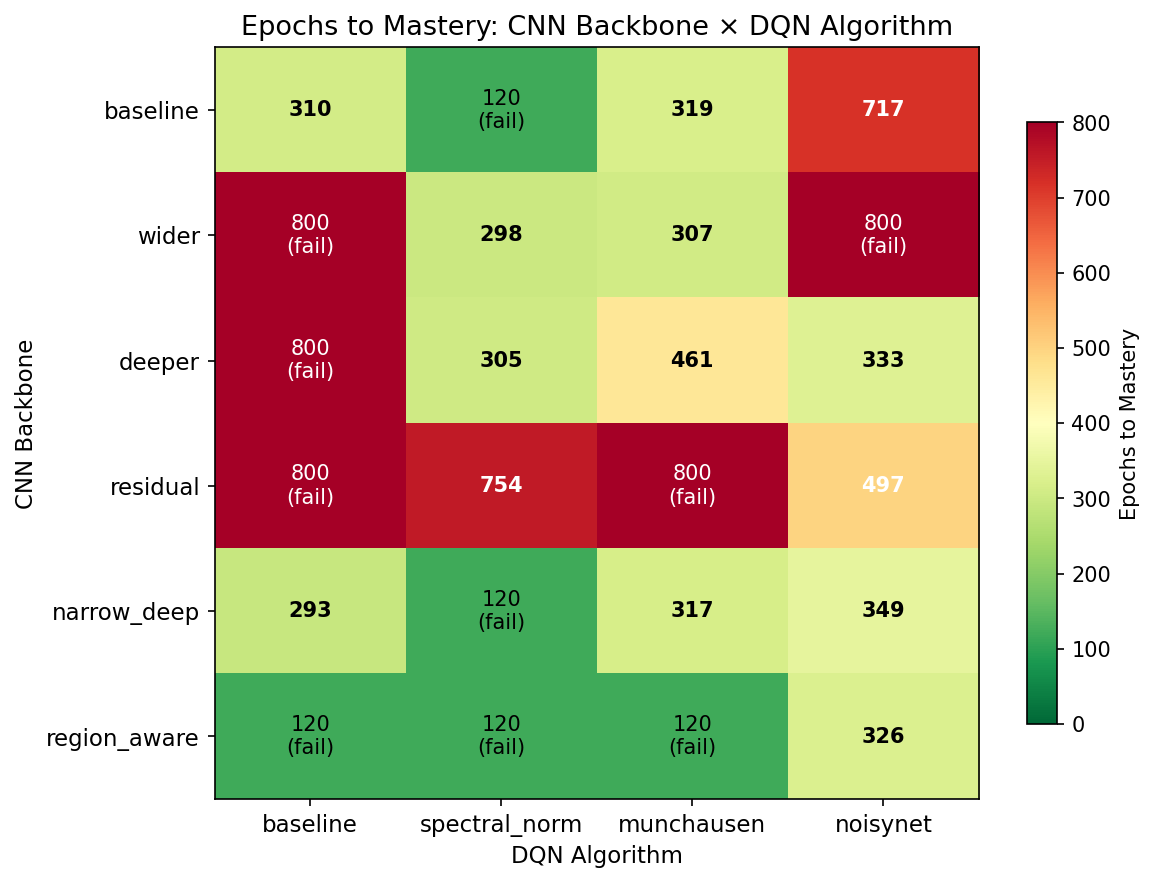
\includegraphics[width=0.85\textwidth]{cnn_dqn_heatmap}
  \caption{Epochs to mastery for all 24 CNN$\times$DQN combinations. Lower values (lighter colours) indicate faster convergence. Cells marked ``fail'' did not achieve full mastery within the 800-epoch budget or were early-stopped at epoch 120.}
  \label{fig:res:cnn_heatmap}
\end{figure}

\textbf{Narrow-Deep dominates on convergence speed.} The smallest backbone (${\sim}43$K params) achieves the fastest mastery with Baseline DQN (293 epochs) and produces three of the ten fastest combinations overall. Contrary to the intuition that larger models learn faster, the Narrow-Deep variant's compact representation appears to regularise learning naturally, avoiding the overfitting or gradient diffusion that plagues larger backbones.

\textbf{The Baseline DQN algorithm shows strong backbone sensitivity.} Baseline DQN achieves the fastest convergence with Narrow-Deep (293 epochs) but fails entirely with Wider (800 epochs), Deeper (800 epochs), and Residual (800 epochs). This suggests that without algorithmic regularisation (Munchausen, Spectral Norm) or adaptive exploration (NoisyNet), the vanilla Baseline algorithm cannot compensate for the optimisation challenges of larger backbones.

\textbf{The Residual backbone is the weakest overall.} Only 2 of 4 combinations achieve mastery, and those require 497 and 754 epochs respectively. The skip connections around the cross-region convolutions appear to dilute the specialised spatial features that the stacked $(3,1,3)$ kernels are designed to extract.

\textbf{Region-Aware succeeds only with NoisyNet.} The structural priors (separate per-region convolutions) help only when paired with NoisyNet's adaptive exploration (326 epochs), failing with all other algorithms. This suggests that the explicit region decomposition constrains the feature space in a way that benefits from noise-driven exploration.

\Cref{fig:res:cnn_bars} shows a grouped bar chart comparing convergence speed across backbones alongside the parameter count for each variant.

\begin{figure}[H]
  \centering
  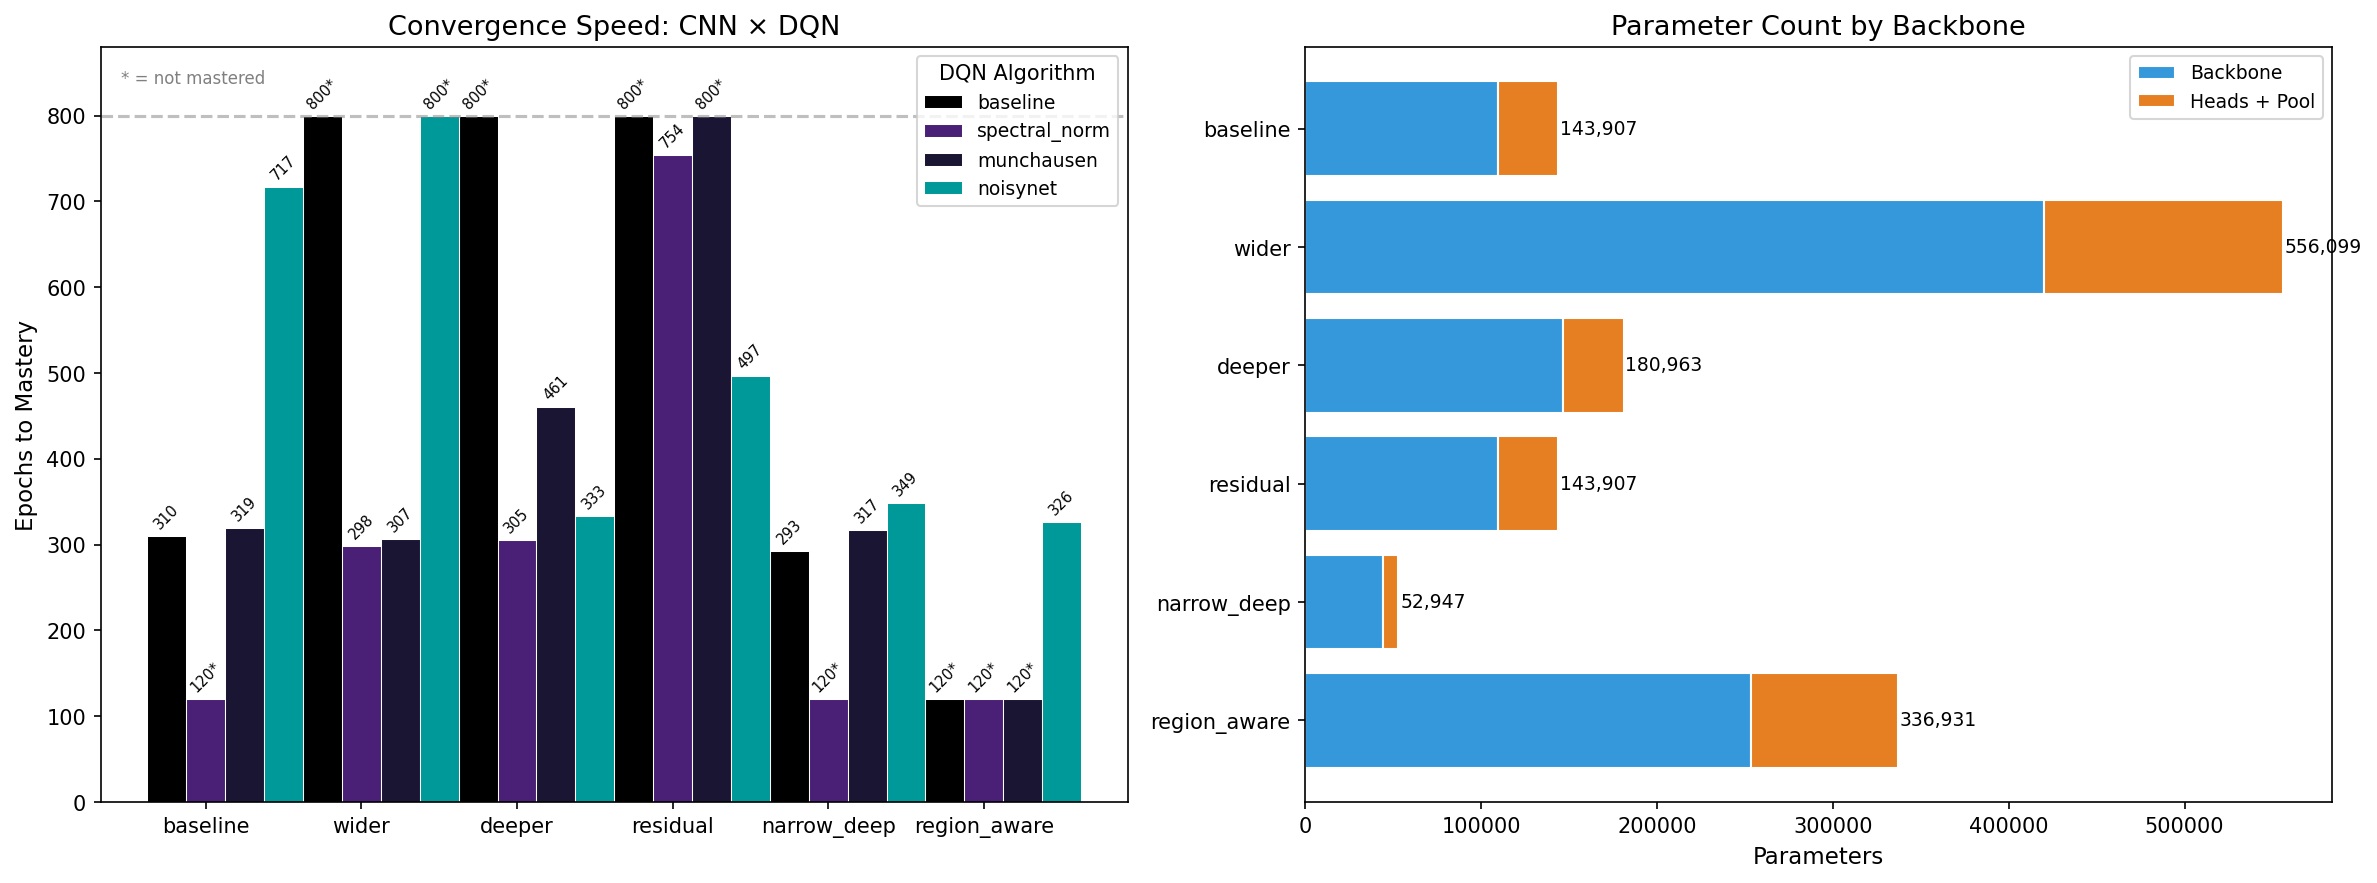
\includegraphics[width=\textwidth]{cnn_dqn_comparison}
  \caption{Left: epochs to mastery grouped by CNN backbone and coloured by DQN algorithm. Bars marked with * did not achieve full mastery. Right: parameter count breakdown showing backbone vs.\ head parameters for each CNN variant.}
  \label{fig:res:cnn_bars}
\end{figure}

\subsubsection{Accuracy Comparison}

While convergence speed measures how quickly each combination learns, the average pass rate at the final epoch indicates how robust the learned policy is. \Cref{fig:res:cnn_accuracy} presents the accuracy heatmap across the $6 \times 4$ grid.

\begin{figure}[H]
  \centering
  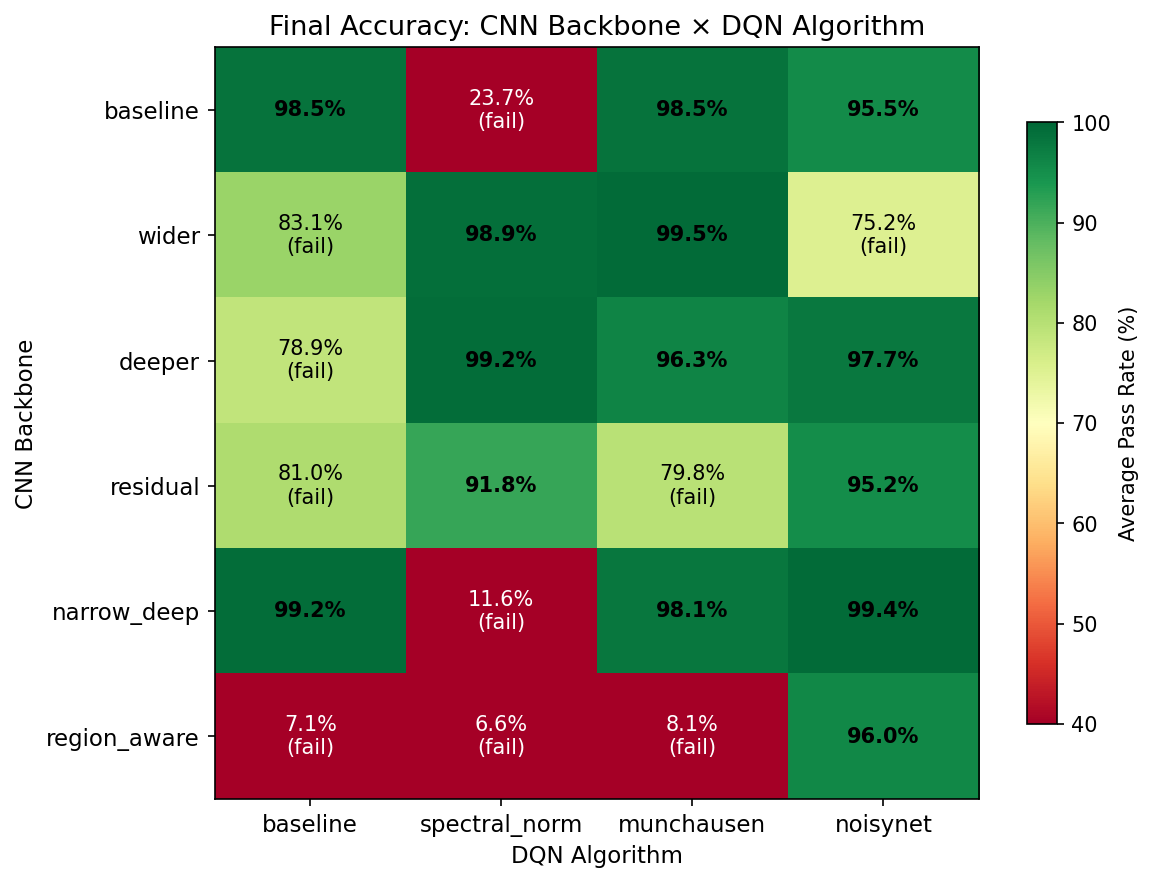
\includegraphics[width=0.85\textwidth]{cnn_dqn_accuracy_heatmap}
  \caption{Average pass rate (\%) across all 31 scenarios for each CNN$\times$DQN combination. Higher values (darker green) indicate more robust final policies. Cells marked ``fail'' did not master all tiers.}
  \label{fig:res:cnn_accuracy}
\end{figure}

The accuracy heatmap reveals a complementary perspective to the convergence analysis. Munchausen+Wider achieves the highest average pass rate (99.5\%), closely matched by Spectral Norm+Deeper and Baseline+Narrow-Deep (both 99.2\%) and NoisyNet+Narrow-Deep (99.4\%). Notably, the fastest combination (Baseline+Narrow-Deep, 293 epochs) also achieves near-best accuracy (99.2\%), breaking the speed-accuracy trade-off observed in Stage~1. This suggests that the Narrow-Deep backbone's compact capacity naturally regularises learning, producing both fast convergence and robust policies.

The failed combinations fall into two distinct patterns. The five early-stopped combinations (epoch 120, $< 24\%$ accuracy) represent fundamental incompatibilities between backbone and algorithm: Spectral Norm fails with Baseline and Narrow-Deep backbones, and all non-NoisyNet algorithms fail with Region-Aware. The five 800-epoch failures (75--83\% accuracy) represent capacity-budget mismatches where the backbone has the representational capacity but the algorithm cannot consolidate learning within the epoch budget.

\subsubsection{Per-Scenario Breakdown}

\Cref{fig:res:cnn_scenarios} provides the full per-scenario pass rate matrix for all 24 combinations, enabling detailed diagnosis of scenario-level failure modes.

\begin{figure}[H]
  \centering
  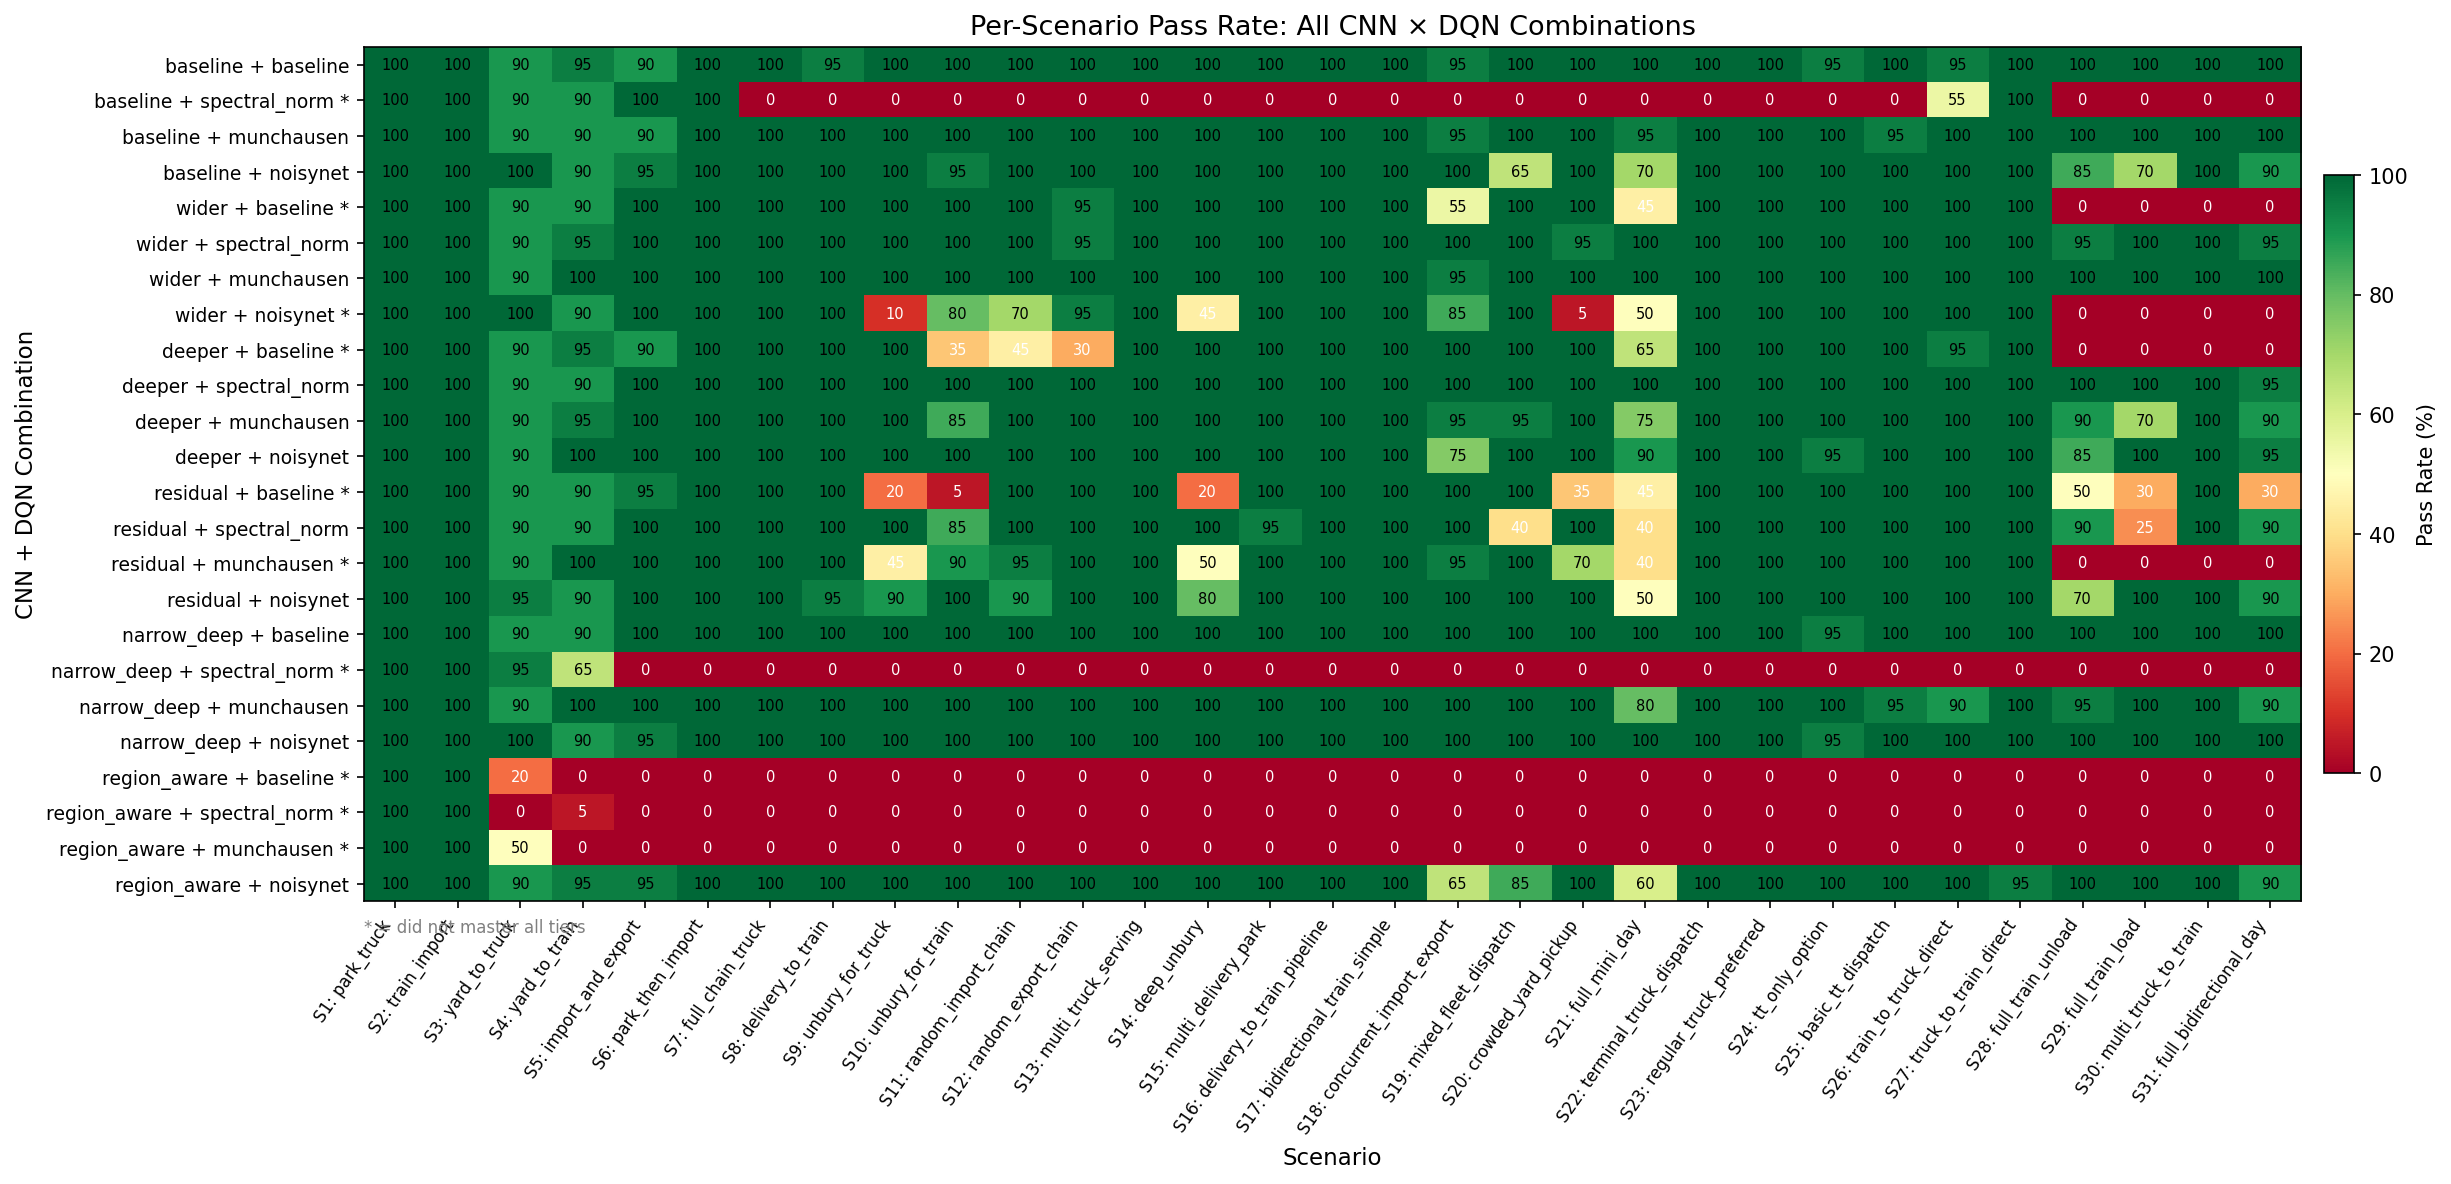
\includegraphics[width=\textwidth]{cnn_dqn_accuracy_scenarios}
  \caption{Per-scenario pass rates for all 24 CNN$\times$DQN combinations. Rows are ordered by backbone then algorithm; columns are the 31 scenarios (S1--S31) grouped by tier. Red cells indicate 0\% pass rate on scenarios in tiers that were never unlocked.}
  \label{fig:res:cnn_scenarios}
\end{figure}

Several diagnostic observations emerge from the scenario-level data:

\begin{itemize}
  \item \textbf{Scenarios S1 through S8, S26, S27} (Tiers~1 through~3: primitives, two-action chains, full chains, direct transfers) are mastered by all 14 successful combinations at $\geq 90\%$ pass rate. These basic logistics operations are learnable regardless of the algorithm-backbone pairing.

  \item \textbf{Scenario S21} (\texttt{full\_mini\_day}, Tier~10) remains the hardest scenario across all combinations. Even among the 14 successful combinations, pass rates range from 70\% to 100\%. This capstone scenario, which requires all logistics skills simultaneously, serves as the strongest differentiator between near-production-ready and merely adequate configurations.

  \item \textbf{Scenarios S28--S31} (Tiers~11--13: full train unload/load, multi-truck-to-train, full bidirectional day) are the new high-complexity scenarios added in the expanded curriculum. These scenarios test sustained multi-step operations with concurrent vehicle traffic. Most successful combinations handle them at $\geq 90\%$, but they contribute to the separation between the top-tier and mid-tier performers.

  \item \textbf{Scenario S14} (\texttt{deep\_unbury}, Tier~5) shows persistent difficulty for several combinations. It requires two sequential restack operations before loading, testing the agent's planning depth. Combinations with lower overall pass rates tend to show the weakest performance here, suggesting that restacking depth is a reliable proxy for general policy quality.
\end{itemize}

% ────────────────────────────────────────────────────────────────
\subsection{Architecture Ranking}
\label{sec:res:phase1:ranking}

Combining both stages, the final architecture ranking considers three criteria: whether the combination achieves full mastery, the number of epochs required, and the final average pass rate. \Cref{tab:res:final_ranking} presents the top five configurations.

\begin{table}[H]
  \centering
  \caption{Top-5 architecture configurations from the two-stage tutorial screening, ranked by a combination of convergence speed and final accuracy.}
  \label{tab:res:final_ranking}
  \begin{tabular}{@{} c l l r r @{}}
    \toprule
    \textbf{Rank} & \textbf{CNN} & \textbf{DQN} & \textbf{Epochs} & \textbf{Avg Rate} \\
    \midrule
    1 & Narrow-Deep   & Baseline      & 293 & 99.2\% \\
    2 & Wider         & Spectral Norm & 298 & 98.9\% \\
    3 & Deeper        & Spectral Norm & 305 & 99.2\% \\
    4 & Wider         & Munchausen    & 307 & 99.5\% \\
    5 & Baseline      & Baseline      & 310 & 98.6\% \\
    \bottomrule
  \end{tabular}
\end{table}
Given the narrow spread in accuracy (98.6–99.5\%), which is well within the run-to-run variance characterised in \cref{sec:res:variance}, the ranking is determined primarily by convergence speed. Accuracy differences at this level are not reliably distinguishable from stochastic noise.

The top five combinations form a remarkably tight cluster: all master the 13-tier curriculum within 293--310 epochs and achieve $\geq 98.6\%$ average pass rate. This convergence of results across different backbone-algorithm pairings suggests that the tutorial curriculum has a natural difficulty ceiling that multiple architectures can approach from different directions.

The Baseline+Narrow-Deep combination emerges as the strongest candidate, achieving both the fastest convergence (293 epochs) and near-best accuracy (99.2\%) with the smallest backbone (${\sim}43$K parameters). This challenges the assumption that spatial logistics requires large convolutional networks: the compact 6-layer backbone with 16$\to$32 channels apparently captures sufficient spatial features for the task.

Munchausen+Wider achieves the highest absolute accuracy (99.5\%) at only 14 epochs slower, making it the preferred choice when robustness is prioritised over efficiency. The Spectral Norm+Deeper combination matches Narrow-Deep's accuracy (99.2\%) with a larger receptive field, suggesting that cross-region coverage and compact representation are two valid paths to the same outcome.

% ────────────────────────────────────────────────────────────────
\subsection{Stage 3: Extended Scenario Screening (S32--S33)}
\label{sec:res:phase1:stage3}

Stages~1 and~2 screen architectures on the 31-scenario, 13-tier tutorial curriculum. However, even the highest-tier scenarios (S30--S31: cross-modal orchestration) exercise specific multi-vehicle patterns in relative isolation. To test whether the top-performing combinations can handle \emph{concurrent multi-modal operations under time pressure}, two additional scenarios are introduced as a 14th tier (Operational Readiness):

\begin{itemize}
  \item \textbf{S32} (\texttt{batch\_train\_loading}): Load 10 export containers onto a train departing in 90~minutes, with 5 import distractors that should be ignored. Tests urgency-driven prioritisation of YARD\_TO\_TRAIN over YARD\_TO\_YARD when the departure window is tight.
  \item \textbf{S33} (\texttt{mixed\_urgency\_ops}): Simultaneously handle 5 exports to train, 5 imports from train to yard, and 3 delivery truck park-and-unload operations. Tests interleaving of PARK\_TRUCK, TRUCK\_TO\_YARD, TRAIN\_TO\_YARD, and YARD\_TO\_TRAIN without falling into reshuffle loops.
\end{itemize}

Ten combinations were selected for this extended screening from the 14 Stage~2 successes: those with similar convergence speeds (within approximately 60 epochs of each other), excluding the slowest four that required 461--754~epochs. Each combination was trained on the full 14-tier curriculum (33 scenarios) for up to 150~epochs. \Cref{tab:res:stage3_results} reports the outcomes.

\begin{table}[H]
  \centering
  \caption{Stage~3 results: extended screening on the 14-tier curriculum including S32 and S33. ``Stage~2 Rank'' refers to the convergence ranking from \cref{tab:res:cnn_summary}. Failed combinations plateaued at approximately 80\% completion after 150~epochs.}
  \label{tab:res:stage3_results}
  \begin{tabular}{@{} c l l l r @{}}
    \toprule
    \textbf{Rank} & \textbf{DQN} & \textbf{CNN} & \textbf{S32/S33} & \textbf{Stage~2 Epochs} \\
    \midrule
    1  & Baseline       & Narrow-Deep    & Passed & 293 \\
    3  & Spectral Norm  & Deeper         & Passed & 305 \\
    5  & Baseline       & Baseline       & Passed & 310 \\
    7  & Munchausen     & Baseline       & Passed & 319 \\
    10 & NoisyNet       & Narrow-Deep    & Passed & 349 \\
    \midrule
    2  & Spectral Norm  & Wider          & Failed (${\sim}$80\%) & 298 \\
    4  & Munchausen     & Wider          & Failed (${\sim}$80\%) & 307 \\
    6  & Munchausen     & Narrow-Deep    & Failed (${\sim}$80\%) & 317 \\
    8  & NoisyNet       & Region-Aware   & Failed (${\sim}$80\%) & 326 \\
    9  & NoisyNet       & Deeper         & Failed (${\sim}$80\%) & 333 \\
    \bottomrule
  \end{tabular}
\end{table}

Five of the ten combinations master S32 and S33. The five that fail plateau at approximately 80\% completion after 150~epochs --- close to but not reliably above the 90\% mastery threshold. Retries with different seeds occasionally push these closer to 90\%, suggesting that the failures reflect insufficient convergence velocity rather than fundamental incapacity.

The most striking finding is a \textbf{reversal of the Stage~2 ranking}. The Wider backbone, which produced two of the top-5 combinations in Stage~2 (ranks~2 and~4), fails on both entries in Stage~3. Meanwhile, NoisyNet+Narrow-Deep (rank~10) and Munchausen+Baseline (rank~7) --- neither in the original top-5 --- pass comfortably. This indicates that convergence speed on the 13-tier curriculum is a necessary but not sufficient predictor of generalisation to operational-complexity scenarios.

\subsubsection{Backbone-Level Analysis}

The Stage~3 outcomes reveal a clear backbone-level pattern:

\begin{itemize}
  \item \textbf{Baseline CNN (2/2 pass):} The most robust backbone. The moderate-capacity 4-layer architecture (${\sim}108$K backbone parameters) generalises reliably to multi-modal operations regardless of the DQN algorithm.
  \item \textbf{Narrow-Deep (2/3 pass):} Succeeds with Baseline DQN and NoisyNet but fails with Munchausen. The compact backbone generalises well overall, though the interaction with Munchausen's reward shaping creates a fragility that was invisible in Stage~2.
  \item \textbf{Deeper (1/2 pass):} Succeeds with Spectral Norm but fails with NoisyNet. The additional cross-region layer benefits from spectral normalisation's weight constraints under multi-modal time pressure.
  \item \textbf{Wider (0/2 fail):} Both combinations fail. The doubled channel width (${\sim}416$K backbone parameters) that accelerated Stage~2 convergence now appears to overfit to the component-skill patterns, lacking the flexibility to recompose them under concurrent time pressure. This is the strongest per-backbone signal in the screening.
  \item \textbf{Region-Aware (0/1 fail):} The structural region priors that enabled Stage~2 success with NoisyNet do not transfer to scenarios requiring fluid cross-region interleaving.
\end{itemize}

The result reaffirms the value of multi-stage screening: the 13-tier curriculum is necessary to establish component-skill mastery, but an additional operational-complexity gate reveals fragilities that component-skill performance alone cannot predict. The five combinations that pass Stage~3 form the pool from which the Phase~2 agent is selected (\cref{sec:exp:phase2:selection}).

\begin{figure}[H]
  \centering
  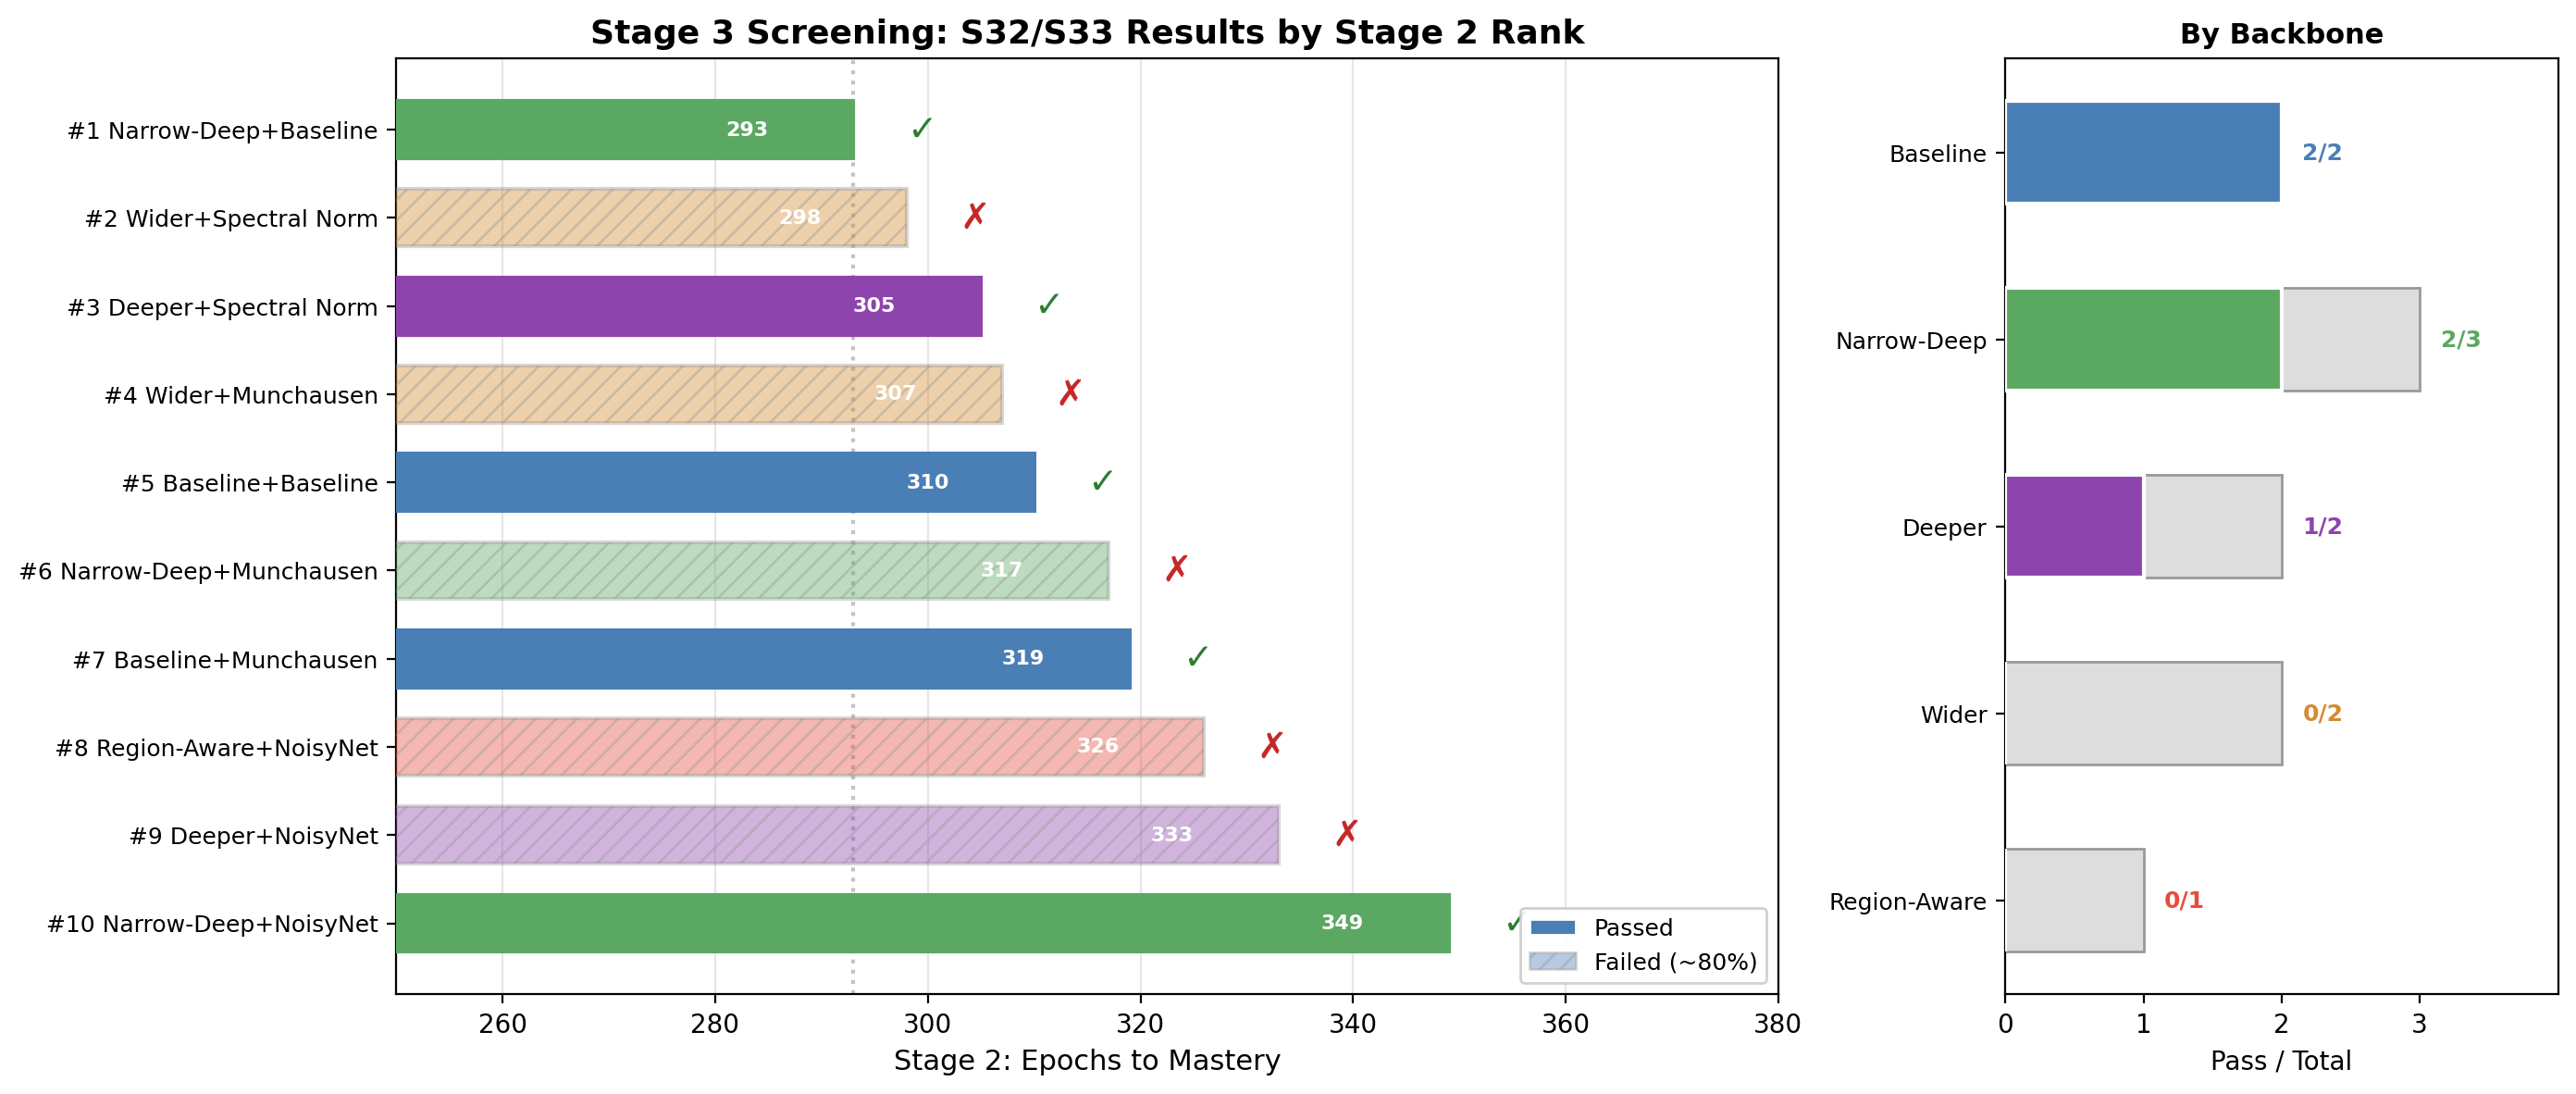
\includegraphics[width=\textwidth]{stage3_results}
  \caption{Stage~3 operational readiness results. Left: the 10 combinations ranked by Stage~2 convergence speed, with pass/fail indicators. Right: summary by backbone showing the number of surviving combinations. Five of ten combinations pass the operational readiness gate.}
  \label{fig:res:stage3_results}
\end{figure}

% ====================================================================
\section{Phase 2: Train-Operation Scalability Results}
\label{sec:res:phase2}
% ====================================================================

Phase~2 addresses RQ2 using the evaluation grid and protocol described in \cref{sec:exp:phase2}.  Six DQN agents and the heuristic baseline (\cref{sec:exp:phase2:selection,sec:exp:phase2:baselines}) are evaluated on the primary train-operation grid (40--400 containers $\times$ three yard fill levels).  A secondary mixed-operation stress test is presented in \cref{sec:res:phase2:stress}.

% ────────────────────────────────────────────────────────────────
\subsection{Scaling Performance}
\label{sec:res:phase2:scaling}
% ────────────────────────────────────────────────────────────────

\Cref{tab:res:phase2_summary} summarises the final-epoch performance of all evaluated agents.  All six DQN agents achieve mean task completion above 93\%, with the top five clustered within two percentage points of each other.  The heuristic baseline never passes a single combination, confirming that the scenarios are not trivially solvable and that the DQN agents have learned genuinely useful policies.

\begin{table}[H]
  \centering
  \caption{Phase~2 agent summary (final warmup epoch, averaged across all 18 parameter combinations).  Completion is the mean fraction of all sub-tasks completed.  Pass rate is the fraction of combinations where \emph{all} sub-tasks reached 100\%.}
  \label{tab:res:phase2_summary}
  \begin{tabular}{@{} l l r r r r @{}}
    \toprule
    \textbf{DQN Variant} & \textbf{CNN Backbone} & \textbf{Completion} & \textbf{Pass Rate} & \textbf{Imports} & \textbf{Exports} \\
    \midrule
    Munchausen     & Baseline    & 97.4\% & 72.2\% & 95.6\% & 99.1\%  \\
    NoisyNet       & Narrow-Deep & 96.2\% & 72.2\% & 92.4\% & 100.0\% \\
    Baseline       & Baseline    & 96.1\% & 55.6\% & 93.9\% & 98.2\%  \\
    Baseline       & Narrow-Deep & 95.9\% & 77.8\% & 92.9\% & 98.9\%  \\
    GRU-DQN        & Narrow-Deep & 95.5\% & 55.6\% & 91.0\% & 99.9\%  \\
    Spectral Norm  & Deeper      & 93.1\% & 33.3\% & 88.8\% & 97.4\%  \\
    \midrule
    \multicolumn{2}{l}{\textit{Heuristic baseline}} & 52.4\% & 0.0\%  & 7.2\%  & 97.6\% \\
    \bottomrule
  \end{tabular}
\end{table}

\begin{figure}[H]
  \centering
  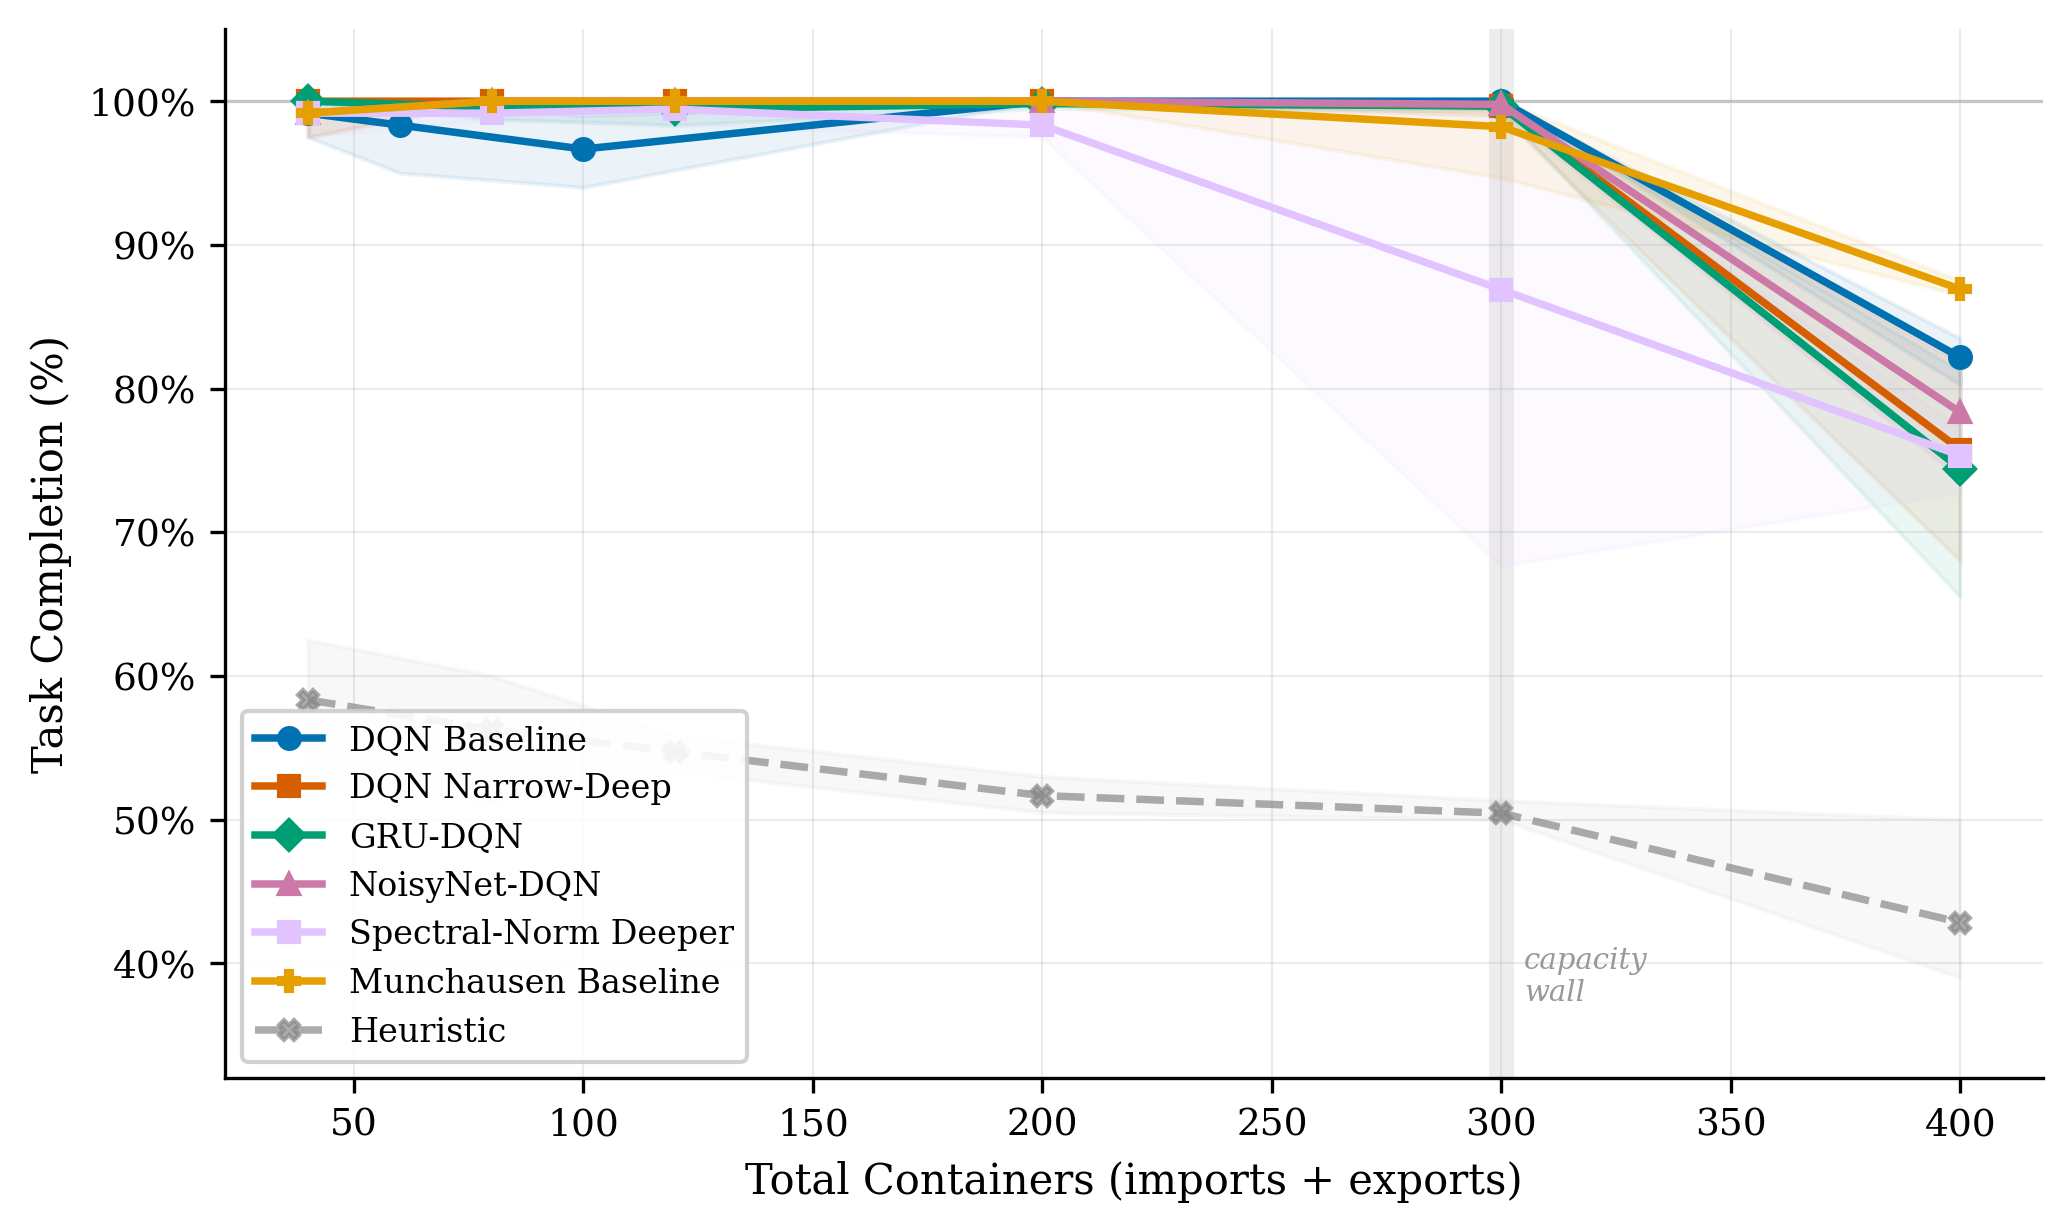
\includegraphics[width=0.9\textwidth]{scaling_curve}
  \caption{Task completion versus scenario size (final warmup epoch).  Solid lines show DQN agents; dashed grey shows the heuristic.  Shaded bands indicate min--max variation across yard fill levels.  All DQN agents maintain $\geq 99\%$ completion up to 200~containers and degrade gracefully beyond 300.}
  \label{fig:res:scaling_curve}
\end{figure}

The scaling curve (\cref{fig:res:scaling_curve}) reveals a clear pattern.  Up to 200~containers, which is ten times the tutorial training scale, all DQN agents maintain near-perfect completion.  Most agents sustain this level at 300~containers as well.  At 400~containers, all agents experience noticeable degradation, though the decline is gradual rather than catastrophic.  The number of required crane moves simply approaches the physical time budget, creating a throughput bottleneck.

\begin{figure}[H]
  \centering
  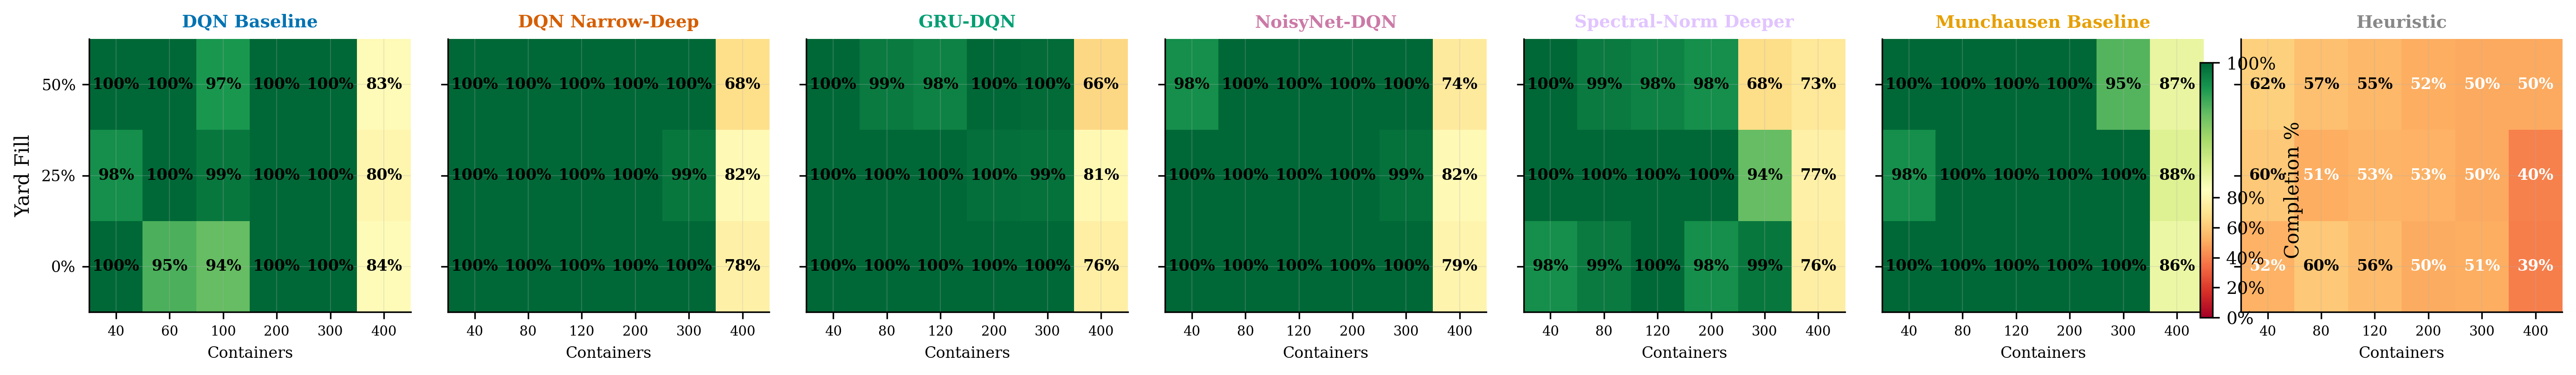
\includegraphics[width=\textwidth]{completion_heatmap}
  \caption{Completion heatmap by container count and yard fill (final warmup epoch).  The diverging colourmap centres on 85\% to highlight where agents begin to struggle.  All DQN agents are uniformly green up to 200~containers; degradation at 400 is visible across all agents.  The heuristic (rightmost panel) is red across the board.}
  \label{fig:res:completion_heatmap}
\end{figure}

The completion heatmap (\cref{fig:res:completion_heatmap}) adds a second dimension by crossing container count with yard fill.  Load size is the dominant performance driver.  Yard fill has a secondary effect that only becomes visible at 300+ containers, where congestion forces additional reshuffles that consume time otherwise spent on productive moves.

\Cref{fig:res:fill_impact} isolates the fill-level effect more precisely.  At 40--200~containers, yard fill has virtually no impact on any agent.  The effect becomes visible at 300~containers and pronounced at 400, where the weaker agents lose up to 10~percentage points when fill increases from 0\% to 50\%.  The mechanism is straightforward: a congested yard forces more reshuffles before the agent can place or retrieve containers, and each reshuffle consumes crane time from a fixed budget.

\begin{figure}[H]
  \centering
  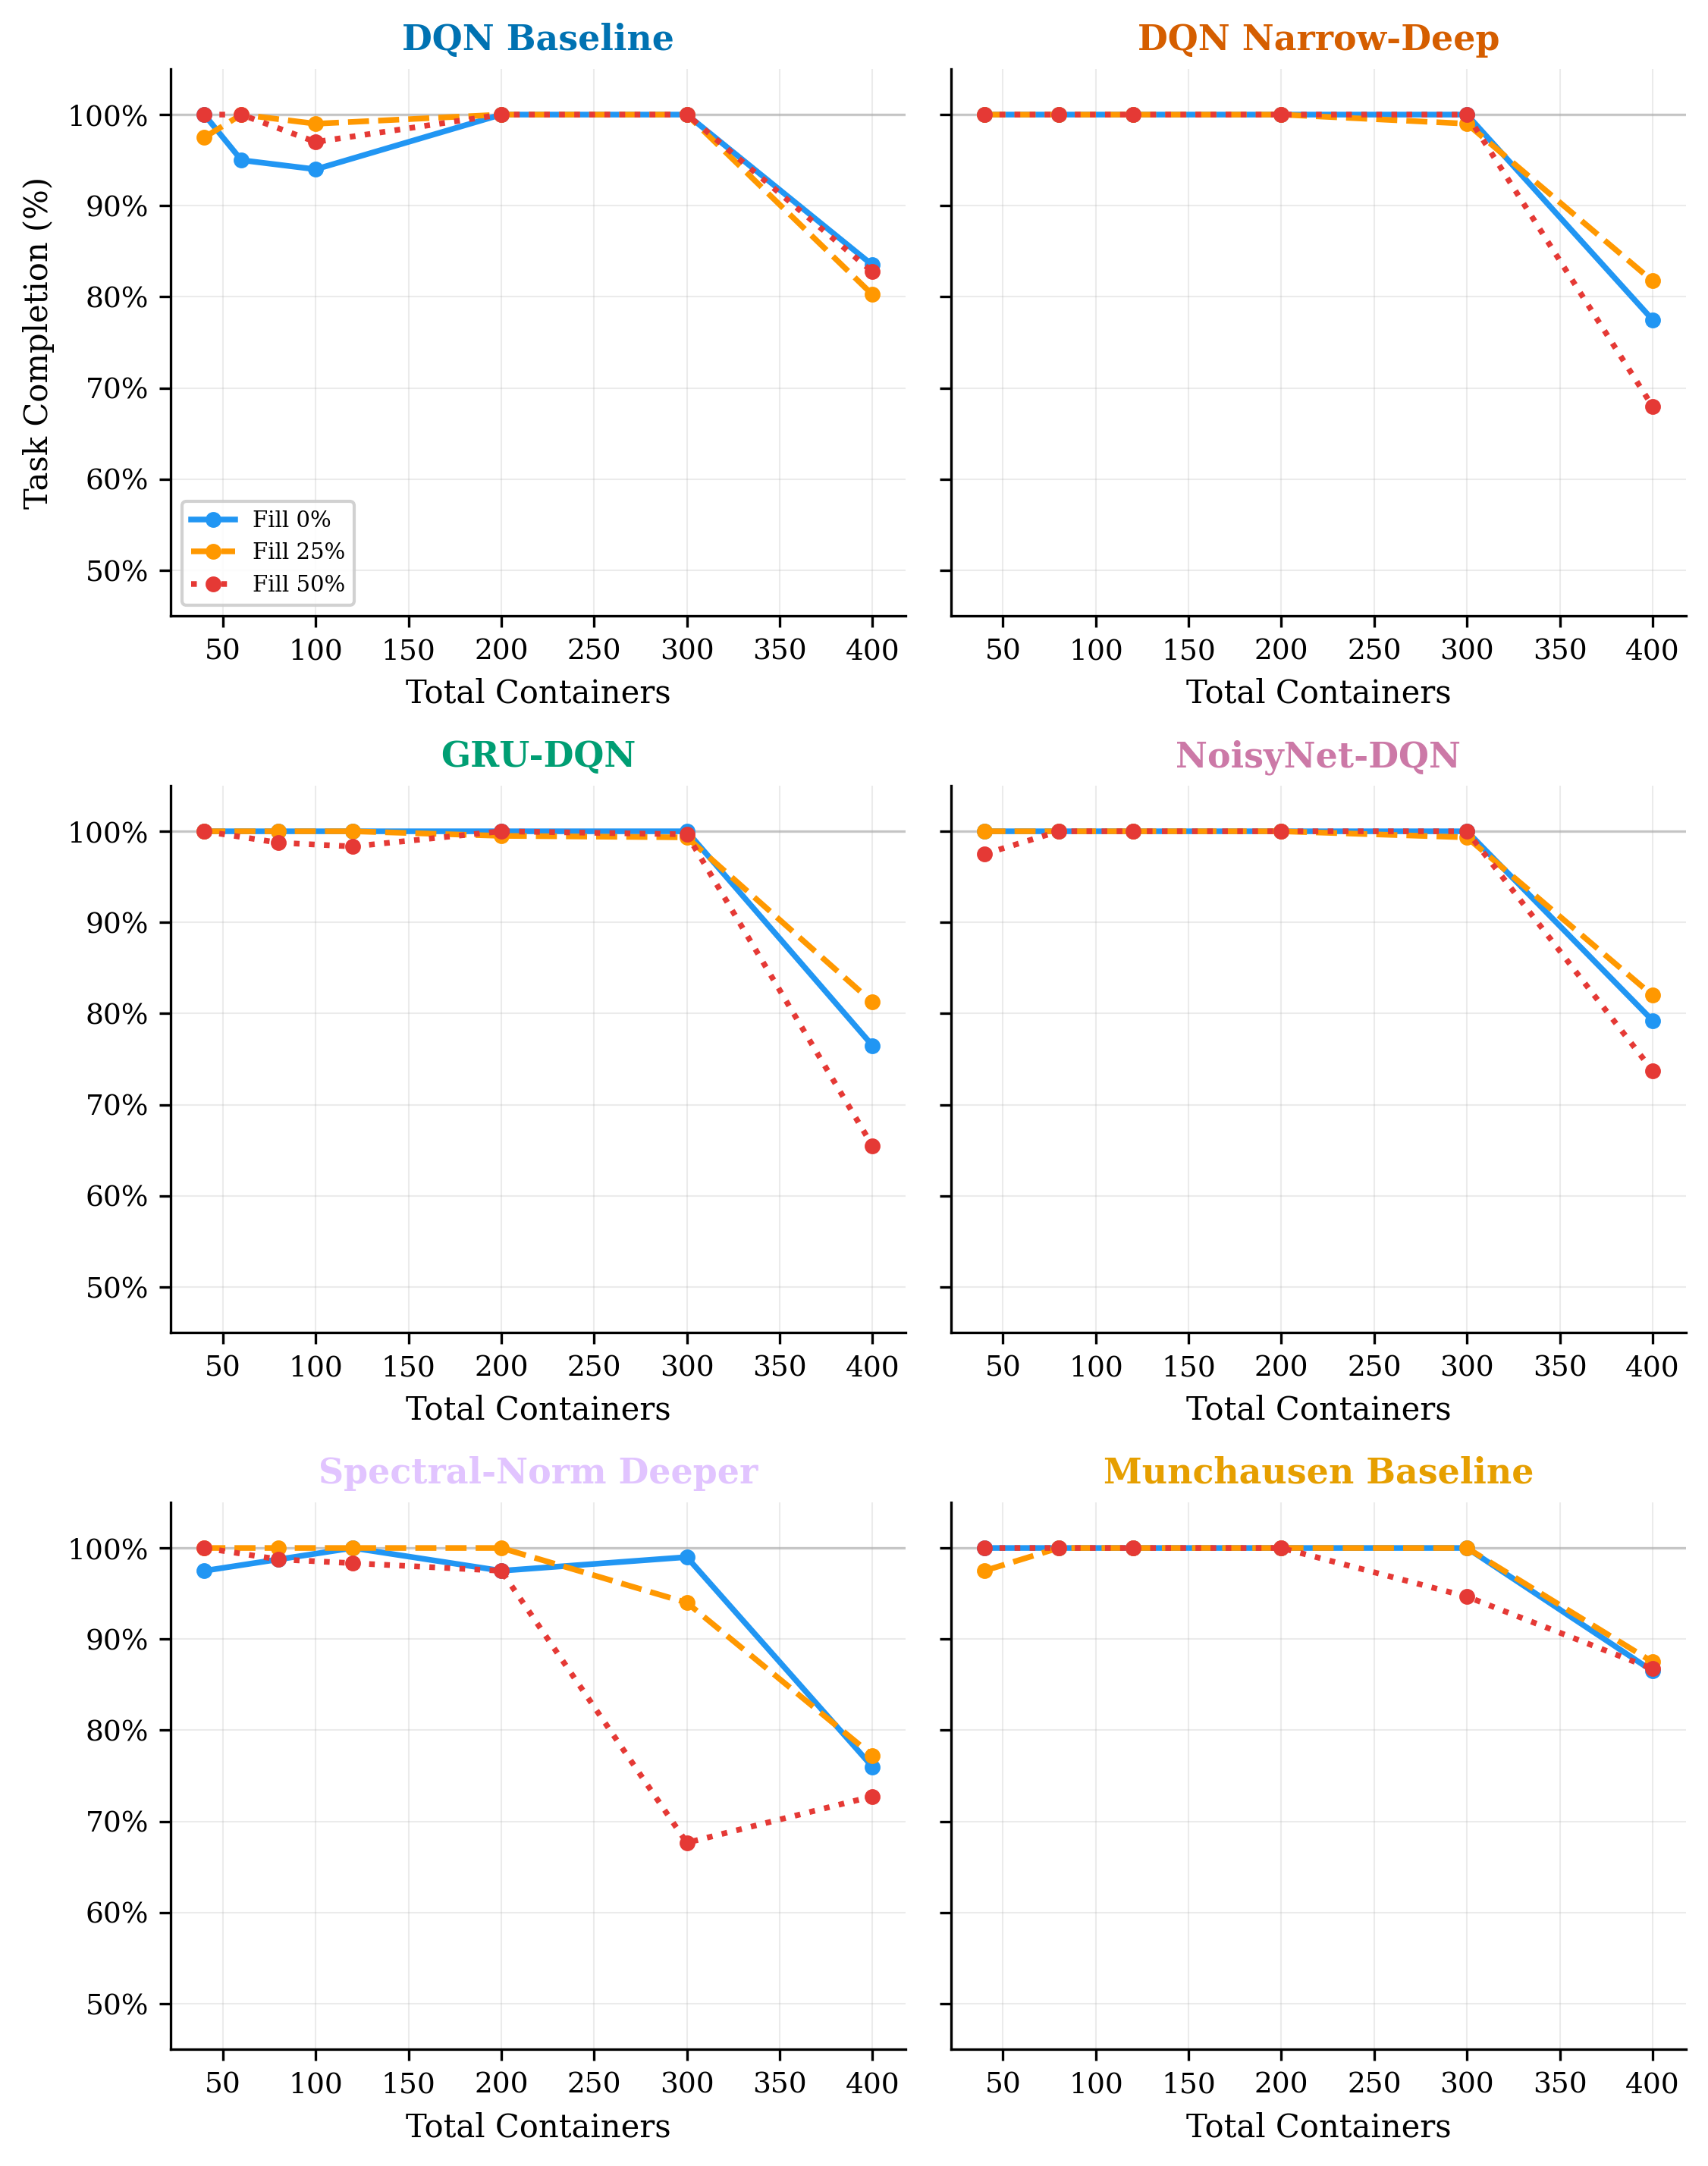
\includegraphics[width=0.95\textwidth]{fill_impact}
  \caption{Impact of yard fill level on task completion across load sizes.  Each subplot shows one scenario size; lines represent individual agents.  Fill level has negligible effect up to 200~containers but increasingly degrades performance at 300--400~containers as yard congestion forces additional reshuffles.}
  \label{fig:res:fill_impact}
\end{figure}

The direct agent comparison (\cref{fig:res:agent_comparison}) confirms that all DQN agents are effectively indistinguishable up to 200~containers.  Differentiation only emerges under pressure: Spectral Norm+Deeper is the first to degrade at 300~containers, while the remaining five agents stay clustered.  At 400~containers the agents spread further apart, but the gaps between them are small relative to the run-to-run variance characterised in \cref{sec:res:variance}.  As with the Phase~1 ranking, a multi-seed evaluation would be needed to establish statistically significant ordering at this frontier.  The heuristic remains far below all learned agents at every scale.

\begin{figure}[H]
  \centering
  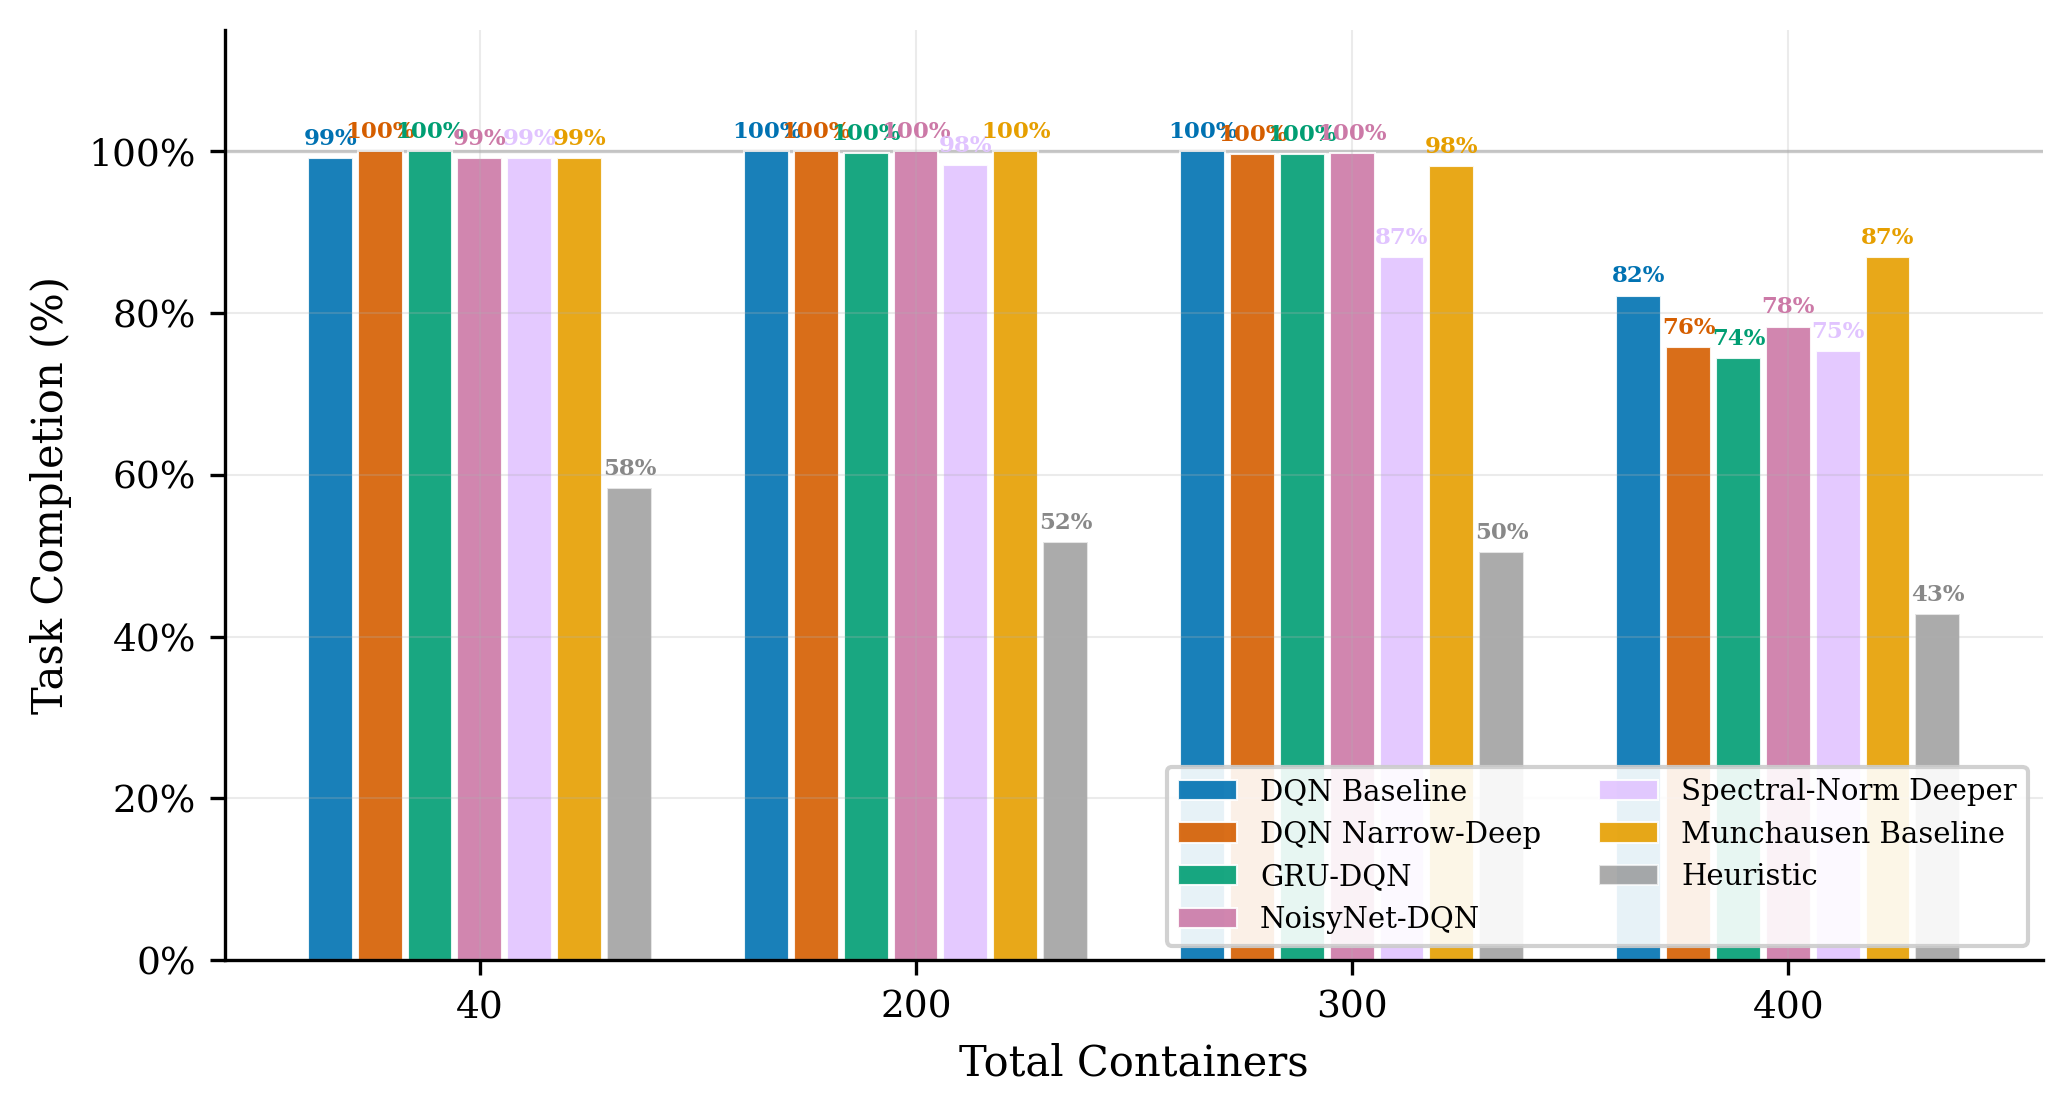
\includegraphics[width=0.9\textwidth]{agent_comparison}
  \caption{Agent comparison: final-epoch completion by scenario size (mean across fill levels).  Grouped bars for the four common scenario sizes.  At 400~containers, Baseline+Baseline leads the DQN agents.}
  \label{fig:res:agent_comparison}
\end{figure}

% ────────────────────────────────────────────────────────────────
\subsection{Import--Export Asymmetry and Task Prioritisation}
\label{sec:res:phase2:asymmetry}
% ────────────────────────────────────────────────────────────────

The most striking finding of Phase~2 is a consistent \textbf{asymmetry between import and export completion} (\cref{fig:res:import_export}).  Across all scenario sizes, every DQN agent maintains near-perfect export completion.  Even at 400~containers, where overall completion drops noticeably, exports remain at or above 97\%.  The performance degradation is driven entirely by imports.

\begin{figure}[H]
  \centering
  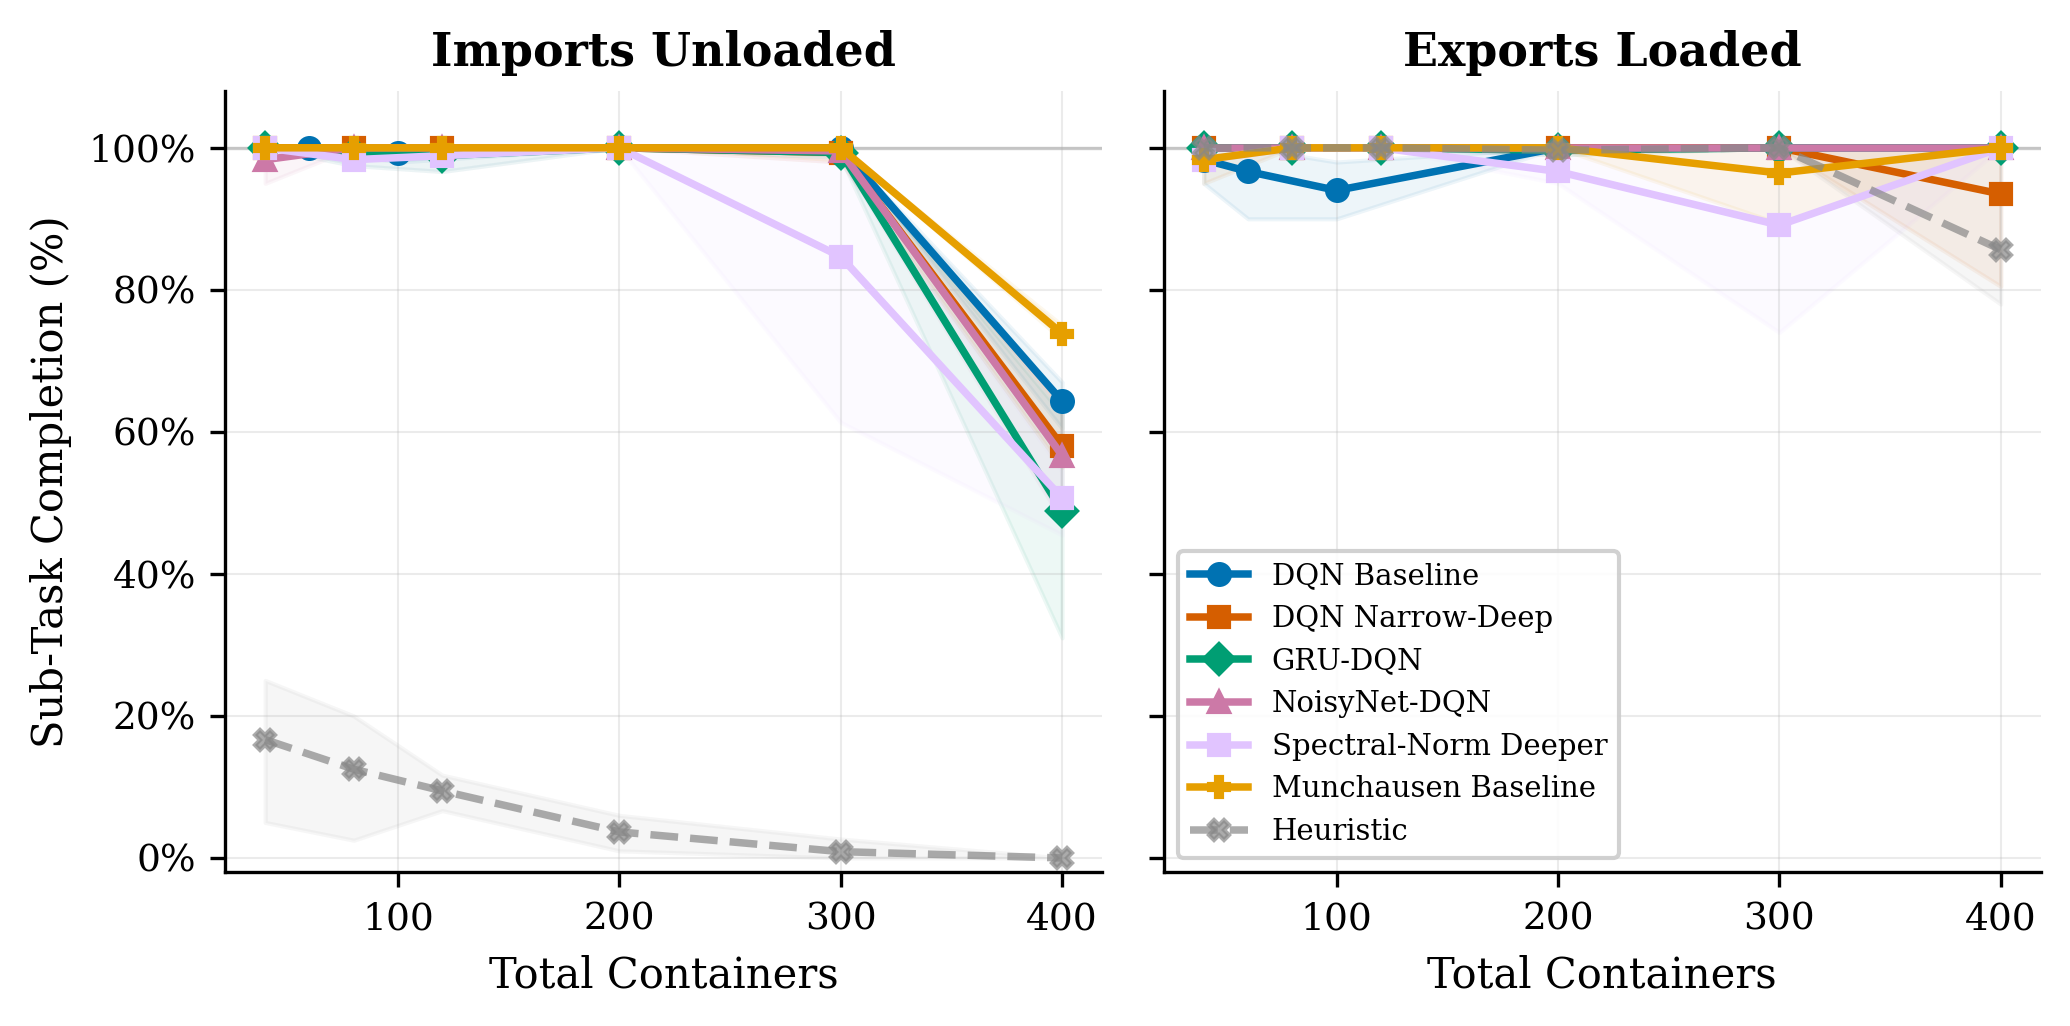
\includegraphics[width=0.9\textwidth]{import_export_asymmetry}
  \caption{Import/export asymmetry (final warmup epoch, mean across fills).  Left: imports unloaded; right: exports loaded.  Exports remain at ${\sim}100\%$ for all DQN agents even at 400~containers, while imports degrade progressively.  The heuristic achieves near-perfect exports but fails imports almost entirely ($\leq 17\%$).}
  \label{fig:res:import_export}
\end{figure}

In practice, a train would not depart with missing containers.  In the simulation, however, the train departs at its scheduled time regardless, and the agent receives a penalty for every container not loaded.  This design choice makes the asymmetry a rational response: exports are time-critical because they must be loaded before departure, while imports can be processed more flexibly.  The agents consistently prioritise YARD\_TO\_TRAIN moves to meet the departure deadline, then use remaining time for TRAIN\_TO\_YARD import unloading.  When the time budget is insufficient for all operations, imports are the rational casualty.

The heuristic baseline exhibits the same asymmetry in a more extreme form.  Its fixed priority order places YARD\_TO\_TRAIN first, which keeps export completion high.  However, its deterministic scan for import placement positions is too rigid for a partially filled yard.  At higher container counts, over half of the heuristic's moves are unproductive YARD\_TO\_YARD reshuffles because it gets trapped in loops, leaving almost no time for actual imports.  The DQN agents avoid this trap by learning to navigate placement decisions spatially through the Q-value landscape.

% ────────────────────────────────────────────────────────────────
\subsection{Move Efficiency}
\label{sec:res:phase2:moves}
% ────────────────────────────────────────────────────────────────

Two efficiency metrics provide insight into how the agents spend their crane time (\cref{fig:res:move_efficiency}).  The \emph{reshuffle ratio} measures what fraction of total moves are YARD\_TO\_YARD reshuffles rather than productive imports or exports.  The \emph{moves per container} ratio measures overall operational efficiency, where the theoretical minimum of 1.0 represents one move per container with no wasted effort.

\begin{figure}[H]
  \centering
  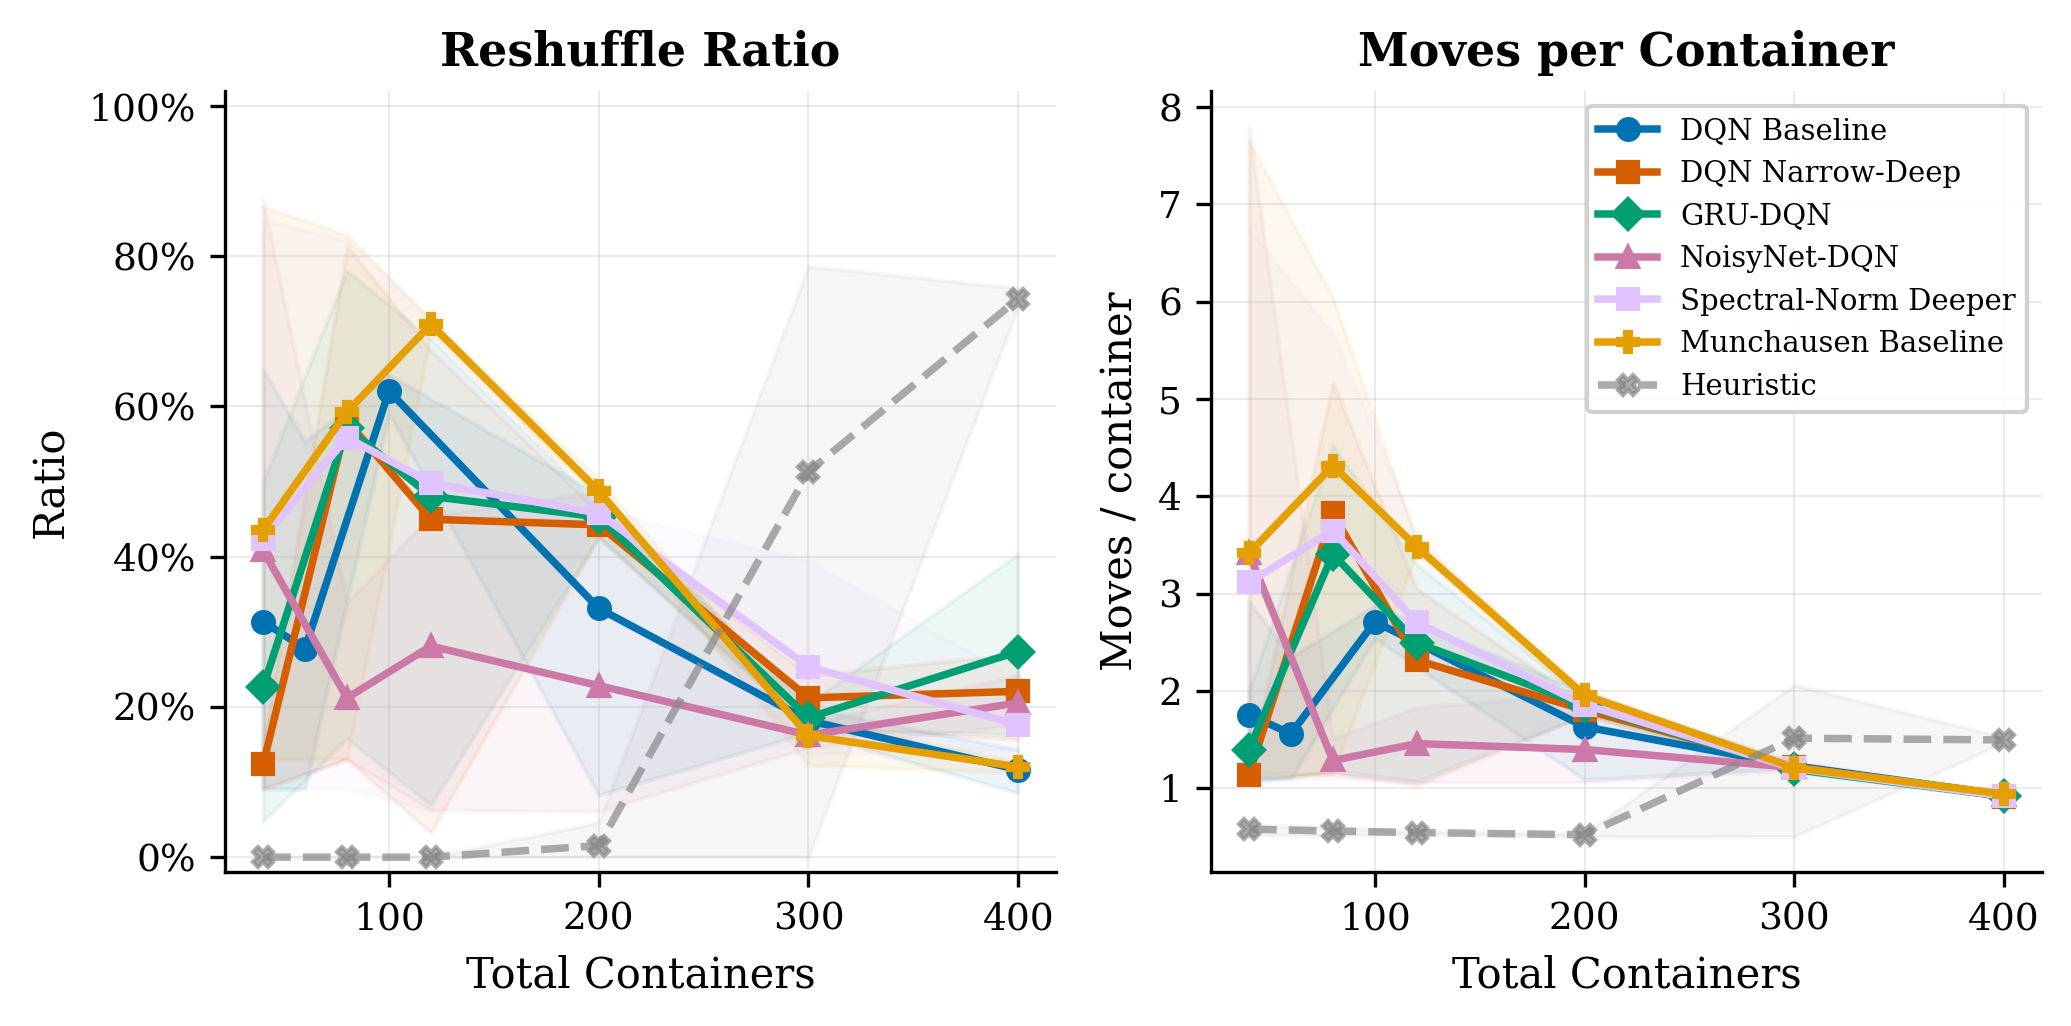
\includegraphics[width=0.9\textwidth]{move_efficiency}
  \caption{Move efficiency metrics (final warmup epoch, mean across fills with min--max band).  Left: reshuffle ratio (lower is better).  Right: moves per container (theoretical minimum is 1.0).}
  \label{fig:res:move_efficiency}
\end{figure}

At small scenario sizes the agents have ample time, and some use it for speculative reshuffles that do not contribute to task completion.  As the scenario size grows, this slack disappears and the agents converge toward efficient behaviour, spending nearly all their crane time on productive moves.  NoisyNet+Narrow-Deep stands out as the most efficient agent across most sizes, while GRU-DQN and Spectral Norm+Deeper tend toward higher reshuffle rates at mid-range scenarios.  At 200--300~containers, all agents achieve 1.2--1.9~moves per container, indicating only moderate overhead above the theoretical minimum.

% ────────────────────────────────────────────────────────────────
\subsection{Learning Dynamics}
\label{sec:res:phase2:learning}
% ────────────────────────────────────────────────────────────────

The warmup learning curves (\cref{fig:res:learning_dynamics}) reveal that the tutorial-learned policies transfer remarkably well to larger scenarios.  Most agents already achieve over 90\% completion on their very first epoch at a new scenario size, and the 30~warmup epochs improve performance by only 1--3 percentage points.  Spectral Norm+Deeper is the sole exception, where cumulative training slightly destabilises its policy.  This pattern validates the Phase~1 curriculum as an effective proxy for scalability: skills learned on 20-container tutorials generalise to 200-container scenarios with minimal adaptation.

\begin{figure}[H]
  \centering
  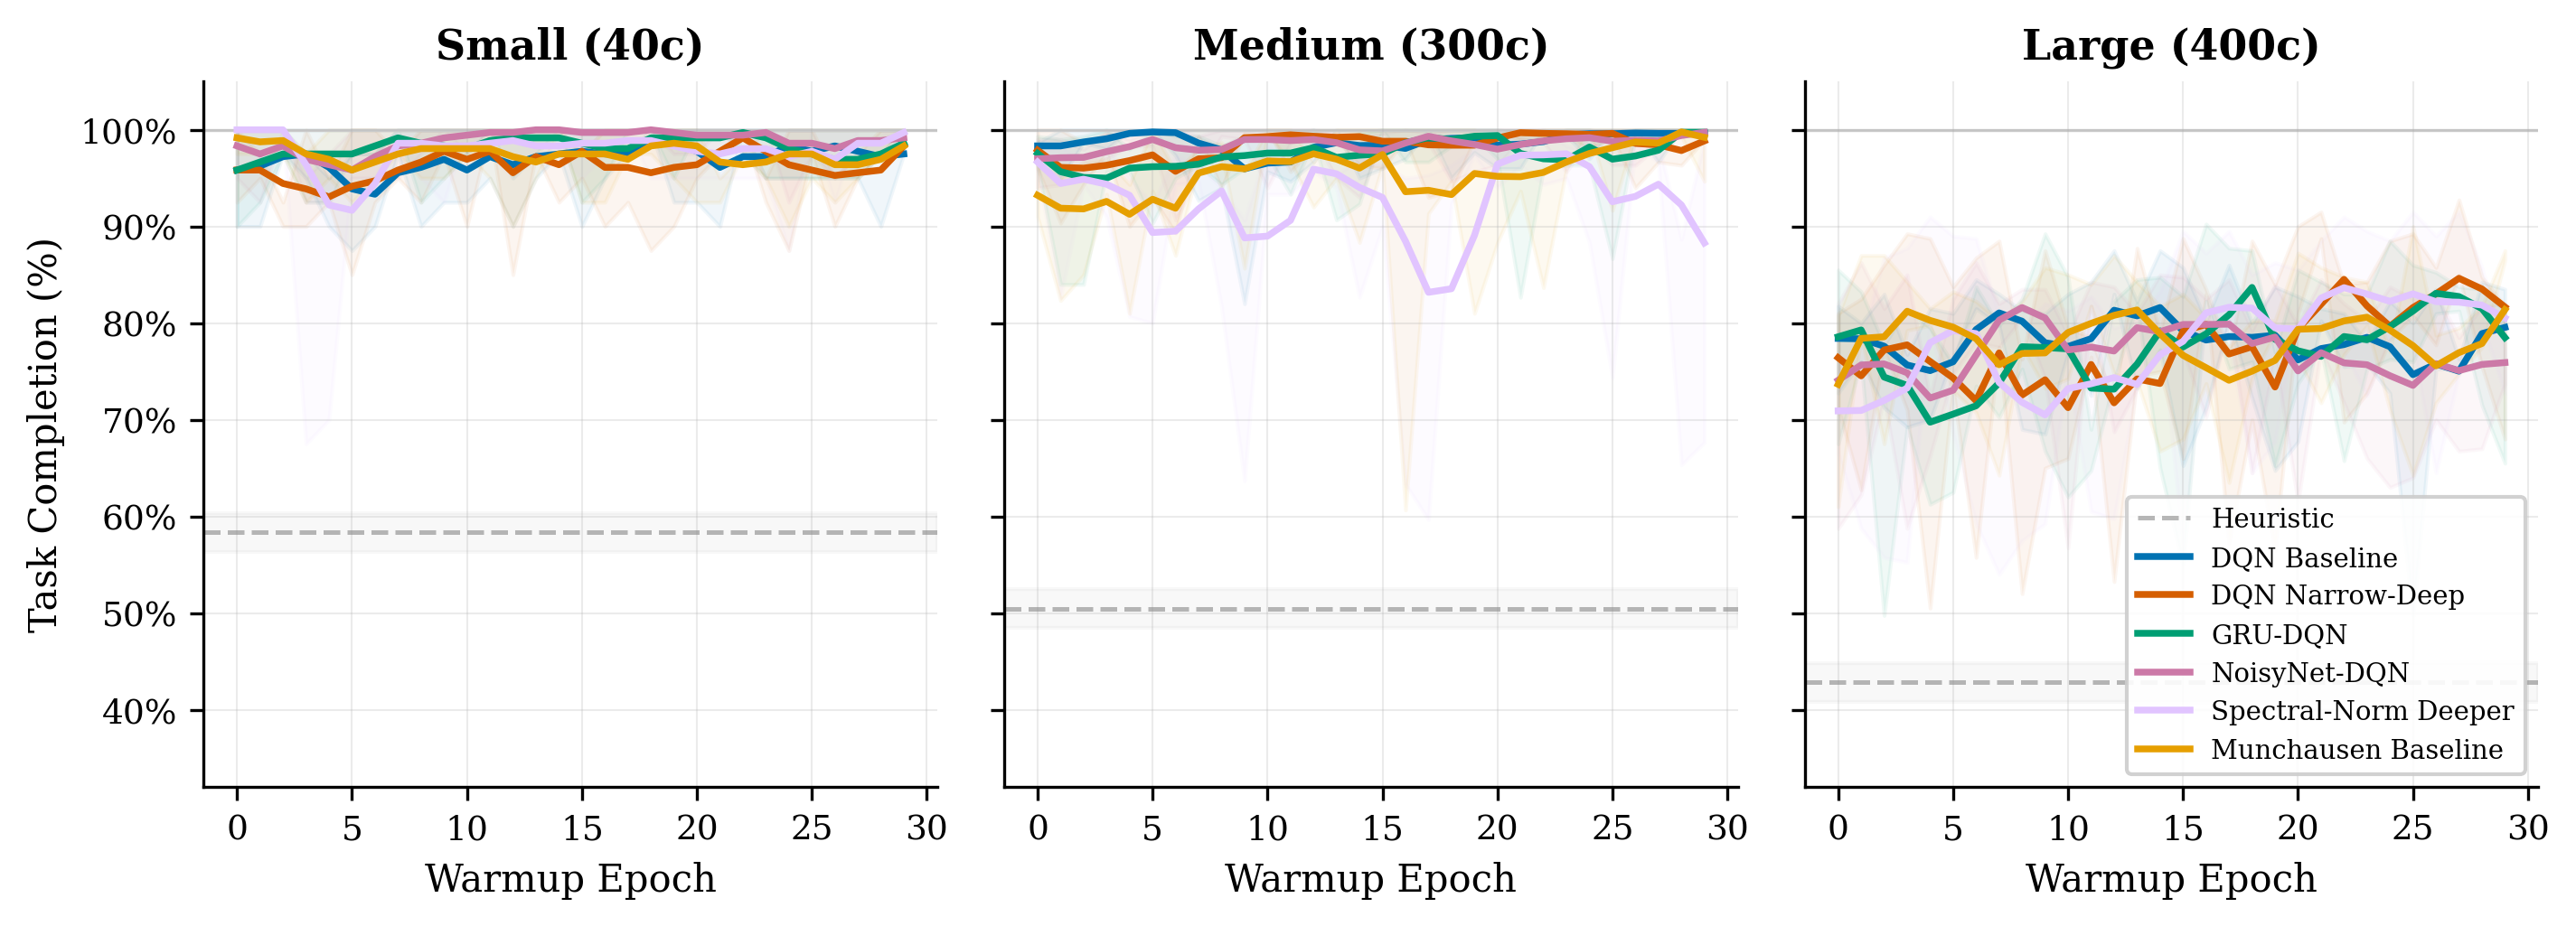
\includegraphics[width=\textwidth]{learning_dynamics}
  \caption{Warmup learning curves for small (40c), medium (200c), and large (400c) scenarios.  Solid lines are DQN agents (mean across fills with min--max band); the dashed grey line is the heuristic.  The DQN agents perform well from the first epoch, indicating strong transfer from tutorials.}
  \label{fig:res:learning_dynamics}
\end{figure}

\textbf{Methodological caveat.}  Because the warmup protocol (\cref{sec:exp:phase2:config}) includes gradient steps, the reported results reflect few-shot adaptation rather than strict zero-shot generalisation.  The small warmup improvement confirms that the vast majority of skill originates from the tutorial curriculum, but readers should interpret the reported completion rates as an upper bound on transfer performance.

% ────────────────────────────────────────────────────────────────
\subsection{Mixed-Operation Stress Test}
\label{sec:res:phase2:stress}
% ────────────────────────────────────────────────────────────────

The primary grid exercises only train operations.  A secondary stress test evaluates whether the Baseline+Baseline agent, the simplest architecture without algorithmic enhancements, can coordinate \emph{all eight move types simultaneously} at scale.  The test uses 100, 200, and 300~containers across two operation mixes (balanced and train-heavy) and three yard fill levels.  Since yard fill has no measurable effect on completion rates,\footnote{One-way ANOVA across the three fill levels yields $p = 0.978$, with a maximum spread of 0.5 percentage points.} the results below are averaged across fill levels.

At 100~containers, the agent handles the full multi-modal workload near-perfectly (\cref{fig:res:stress_heatmap}).  Performance remains strong at 200~containers and degrades moderately at 300, where the coordination overhead of managing all eight move types simultaneously becomes the limiting factor regardless of the train/truck split.

\begin{figure}[H]
  \centering
  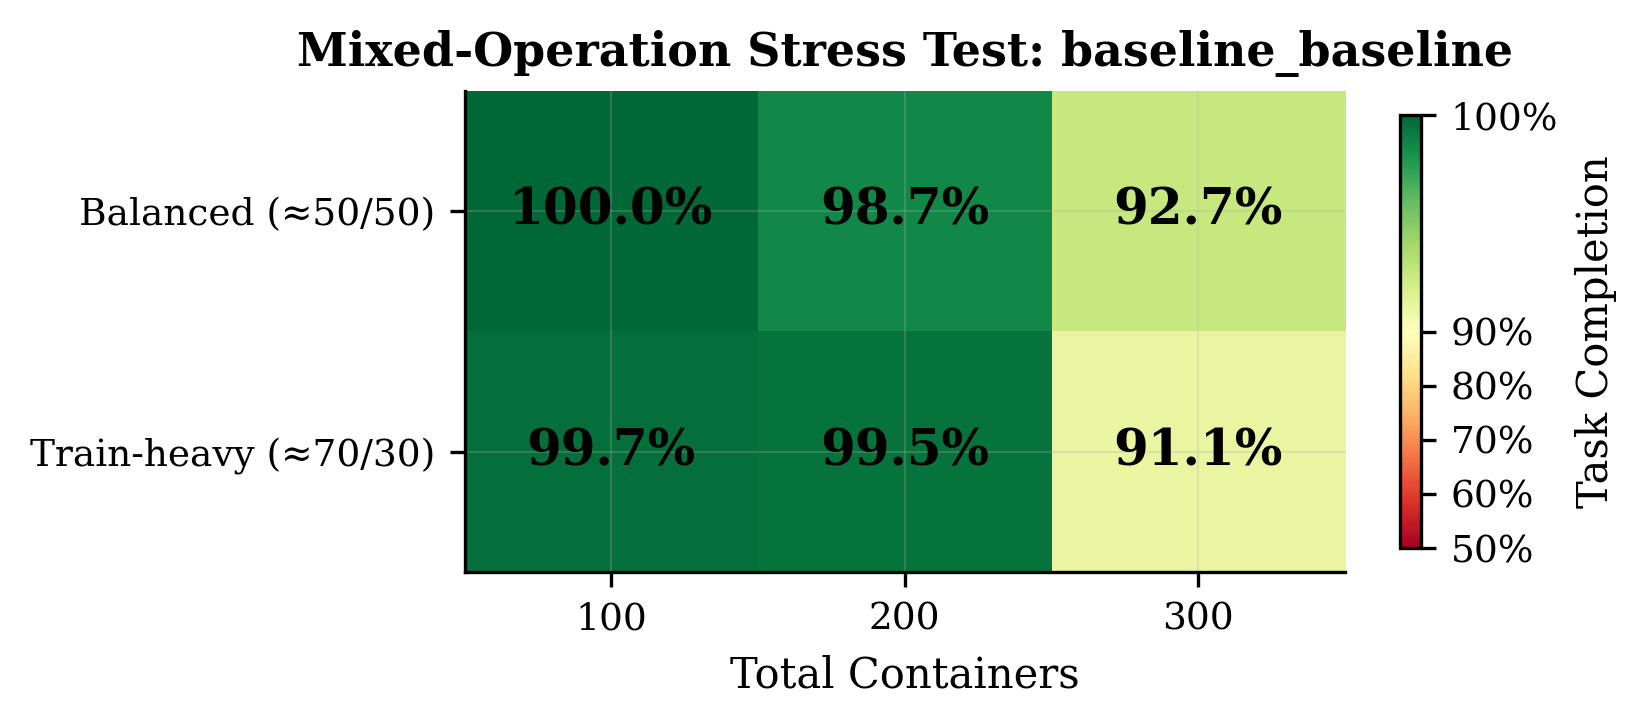
\includegraphics[width=\textwidth]{stress_heatmap}
  \caption{Mixed-operation stress test: completion heatmap for Baseline+Baseline.  Rows represent the two operation mixes (balanced vs.\ train-heavy), columns represent total container count.  Values are averaged across yard fill levels and 30~warmup epochs.}
  \label{fig:res:stress_heatmap}
\end{figure}

The scaling curves for both mixes (\cref{fig:res:stress_ratio}) track each other closely up to 200~containers, then diverge slightly at 300.  Distributing load across train and truck pipelines appears marginally easier than concentrating it on trains alone.  Compared to the train-only evaluation (\cref{fig:res:scaling_curve}), the mixed-operation degradation is smoother and begins earlier, reflecting the additional coordination overhead.

\begin{figure}[H]
  \centering
  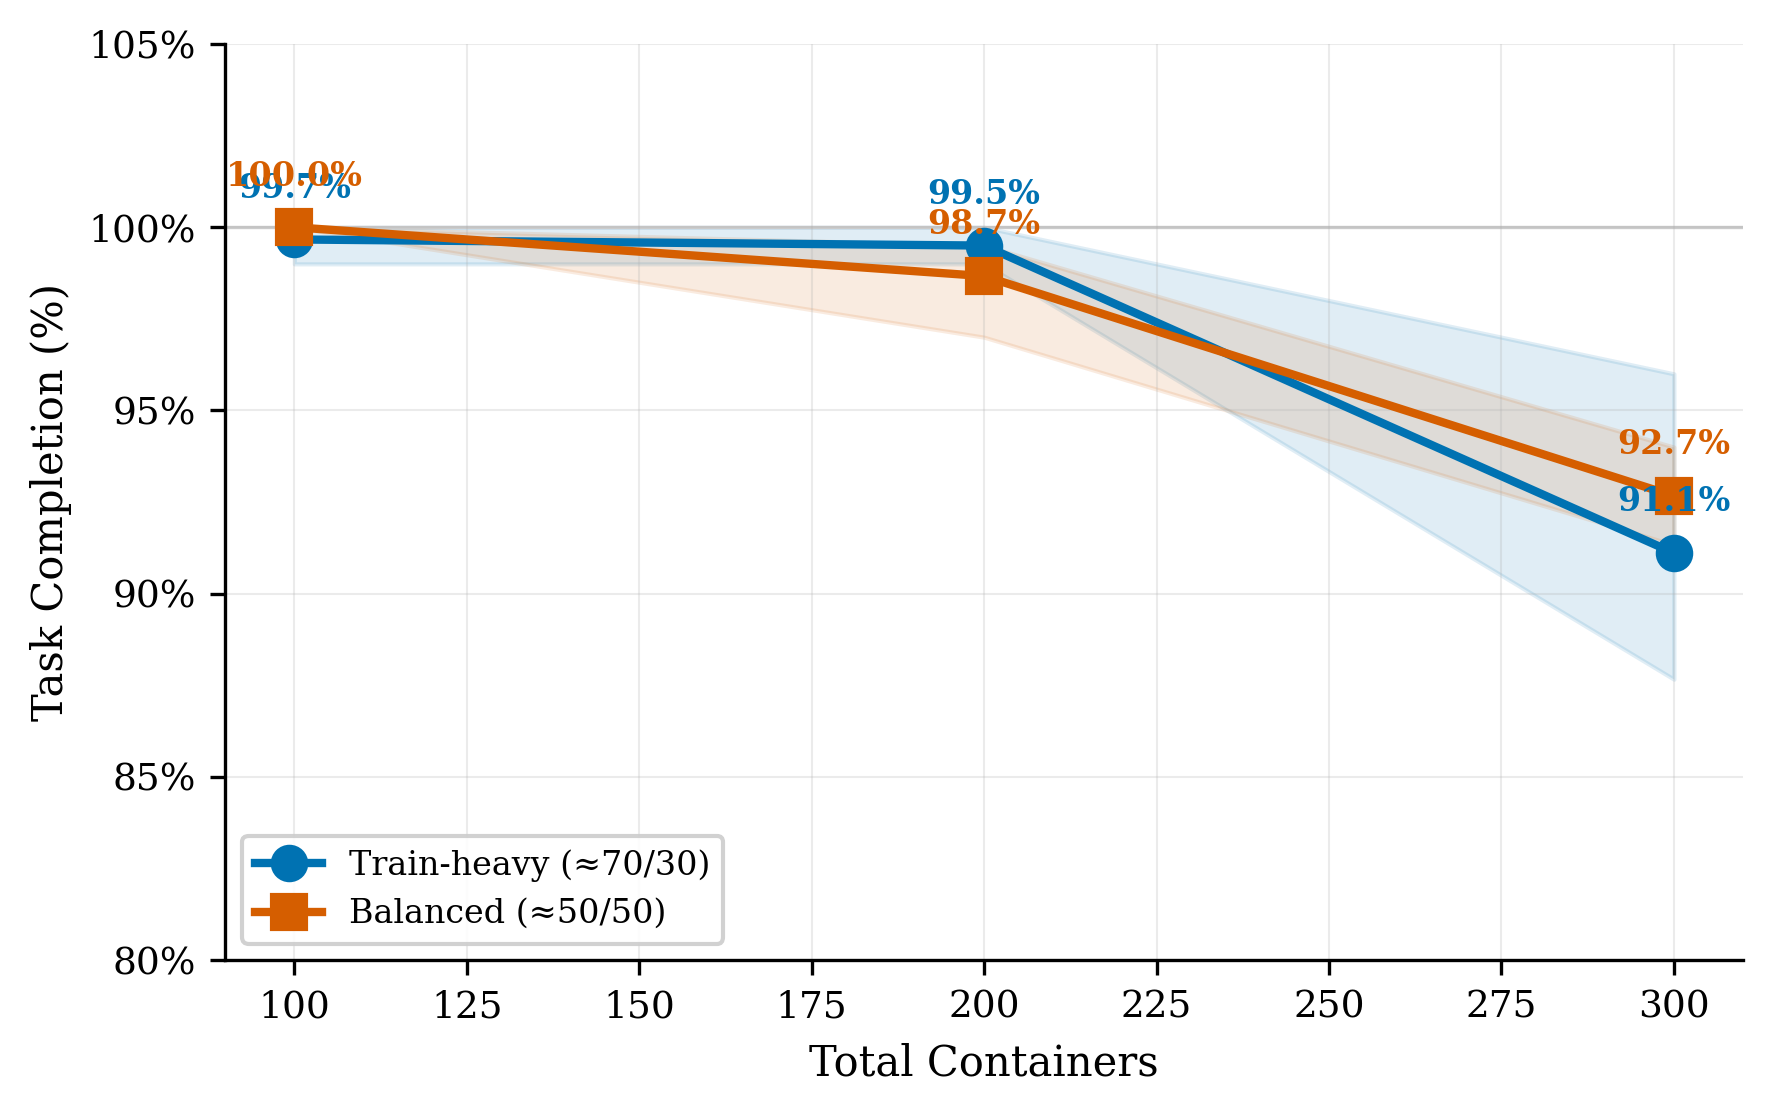
\includegraphics[width=0.9\textwidth]{stress_ratio_impact}
  \caption{Scaling curve for mixed operations: mean task completion versus total container count, separated by operation mix.  Shaded bands indicate the range across yard fill levels.  Both mixes degrade gracefully from ${\sim}100\%$ at 100~containers to ${\sim}91$--$93\%$ at 300.}
  \label{fig:res:stress_ratio}
\end{figure}

\textbf{Sub-task bottleneck analysis.}  Decomposing the balanced-mix results into sub-tasks (\cref{fig:res:stress_subtask}) reveals which operations suffer first under pressure.  At 300~containers, train imports and exports remain largely intact, but truck deliveries and pickups degrade noticeably.  Truck operations require a longer coordination chain (PARK\_TRUCK, then TRUCK\_TO\_YARD or YARD\_TO\_TRUCK), making them the capacity-limiting factor when all move types compete for crane time.  The agent implicitly prioritises train operations, which carry higher reward, over truck service.

\begin{figure}[H]
  \centering
  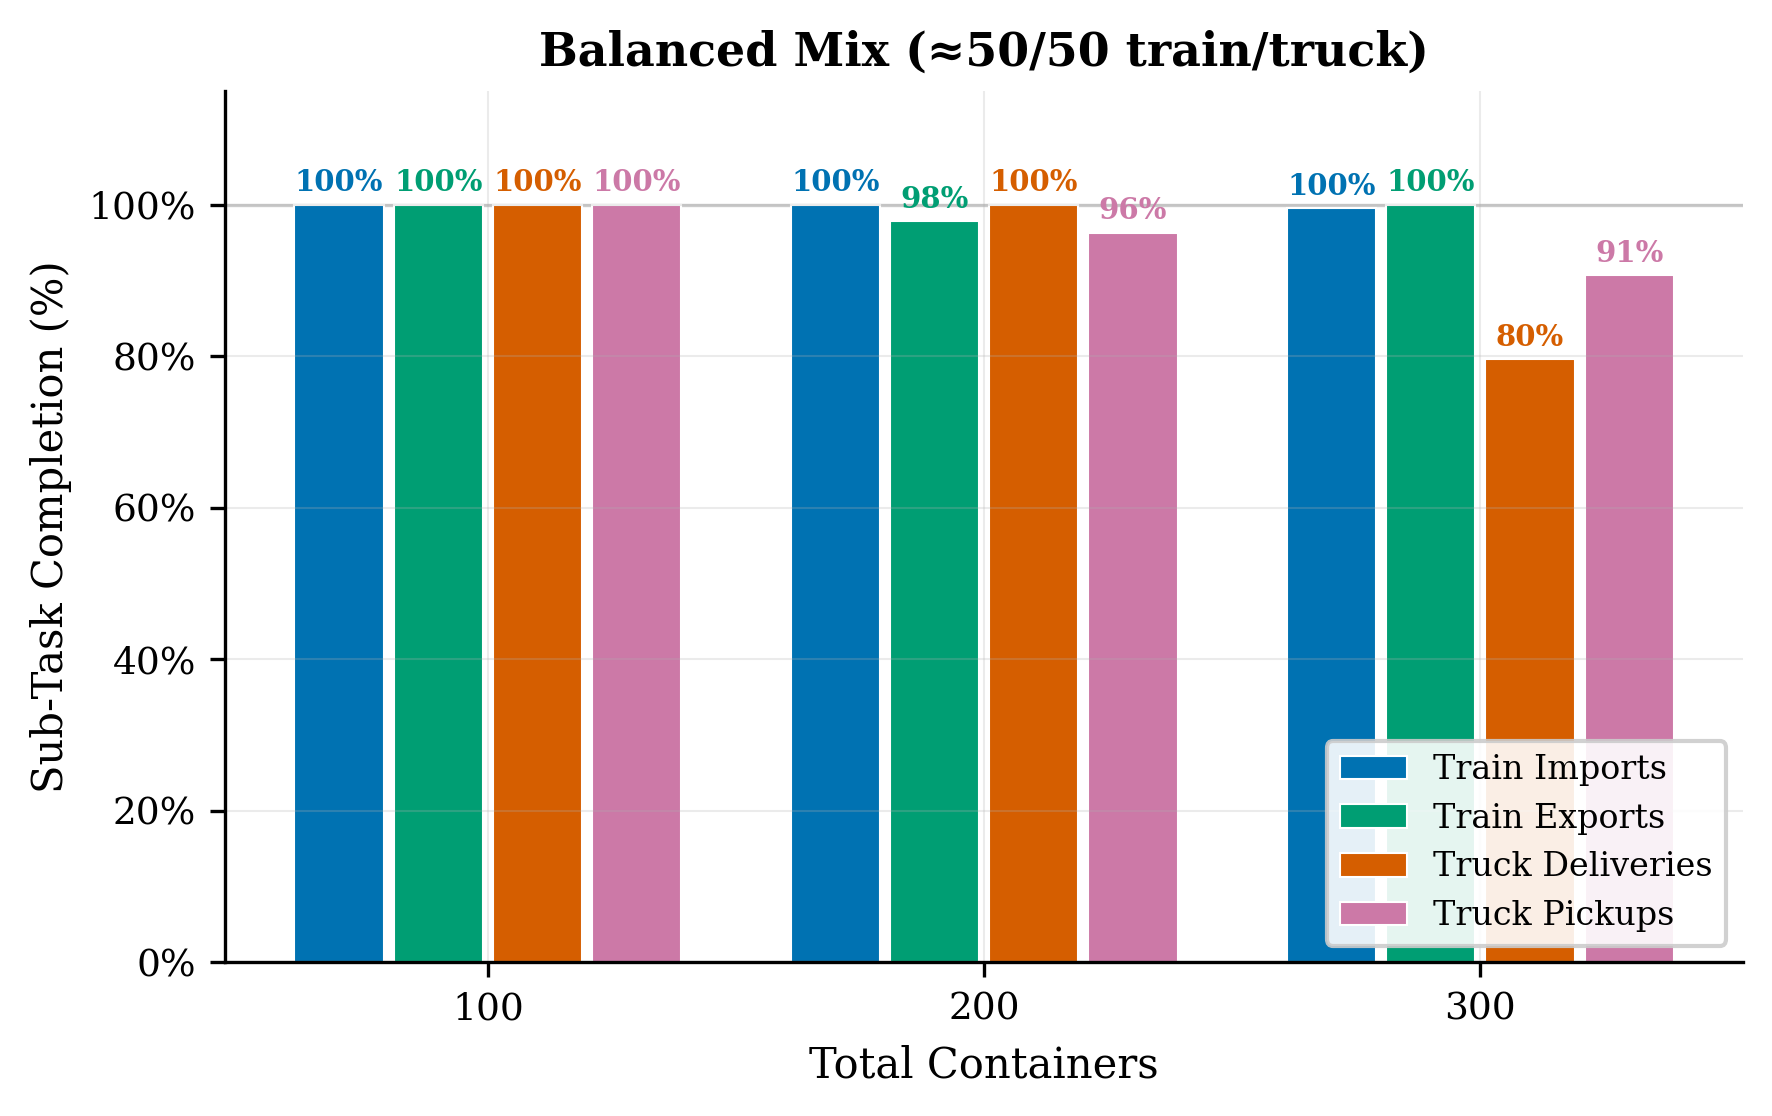
\includegraphics[width=\textwidth]{stress_subtask_breakdown}
  \caption{Sub-task completion breakdown for the balanced (${\approx}50/50$) mix.  Train imports remain at 100\% across all sizes; truck deliveries are the primary bottleneck at 300~containers, dropping to 80\%.}
  \label{fig:res:stress_subtask}
\end{figure}

The stress test demonstrates two key findings.  First, the agent can successfully coordinate all eight move types simultaneously at operational scale, matching the train-only evaluation at 100~containers.  Second, when capacity is exceeded, the agent degrades gracefully and sheds lower-priority truck operations before sacrificing train throughput.  This prioritisation emerges naturally from the reward hierarchy rather than from explicit programming.  The finding aligns with the reactive dispatcher characterisation from \cref{sec:disc:interpretation:scalability}: the agent handles each individual decision competently, but the accumulated coordination overhead of context-switching between eight move types limits throughput at scale.

% chapters/10_discussion.tex
\chapter{Discussion}
\label{ch:discussion}

\section{Interpretation of Results}
\label{sec:disc:interpretation}

The central question (\cref{sec:intro:rqs}) receives a qualified \emph{yes}. Phase~1 demonstrates that compositional mastery of sub-tasks, built through the tiered curriculum, produces agents capable of joint terminal operations in controlled settings (\cref{sec:res:phase1}). Phase~2 confirms that this compositional skill scales well beyond the training distribution (\cref{sec:res:phase2}), and the mixed-operation stress test shows that all eight move types can be coordinated simultaneously at operational scale (\cref{sec:res:phase2:stress}). The following sections examine what the agent has and has not learned, and where the methodology's limits lie.

\subsection{What the Agent Learned}
\label{sec:disc:interpretation:learned}

The Phase~1 results (\cref{sec:res:phase1}) show that the spatial DQN agents learn correct spatial reasoning for single-step decisions: selecting the right source container, choosing an appropriate destination, and coordinating movements across facility regions. Four CNN$\times$DQN combinations master all 33 tutorial scenarios, including cross-region transfers that require the CNN to extract features spanning multiple regions of the state tensor. The escape velocity experiment (\cref{sec:res:variance:escape}) further suggests that IQN may also be viable, as it escapes Tier~0 in 9 of 10 multi-seed runs despite its single-seed failure.

Beyond correct execution, two emergent strategies appear in the learned policies that were never explicitly rewarded. First, agents learn \emph{proximity-aware placement}: when importing containers from trains, they prefer yard positions near the rail region, reducing crane travel for future exports. This behaviour is visible in the destination Q-value heat maps, where Q-values peak in yard rows adjacent to the rail tracks. Second, agents develop a preference for keeping the yard ``flat'' by distributing containers across bays rather than stacking to maximum tier, which reduces future restacking. Both strategies emerge from the combination of the distance penalty in the reward function (\cref{app:reward}) and the multi-step return, which propagates the cost of future reshuffles back to the placement decision that caused them.

Early in training, agents exhibit excessive YARD\_TO\_YARD shuffling on restacking scenarios such as S9 and S10, sometimes executing 40--60 reshuffles without transitioning to the actual delivery move. This behaviour largely disappears as training progresses and the policy internalises the correct sequencing. The scenarios where it persists in greedy evaluation (\cref{sec:res:phase1:dqn}) point to a structural limitation: without temporal context, the agent has no mechanism to encode a multi-step intention such as ``restack to access container~X for Train~2.'' Each decision is made from a static snapshot, making the agent reactive rather than strategic.

The heuristic baseline (\cref{sec:res:phase2:scaling}) provides evidence that the learned policies reflect genuine spatial skill rather than reward exploitation. The heuristic follows the same priority ordering that the reward function encodes, yet achieves only 52.4\% mean completion compared to the Munchausen agent's 97.4\%. Both have access to identical objective priorities, but the heuristic lacks the spatial reasoning to navigate yard congestion or coordinate multi-step transfers. This 45-percentage-point gap demonstrates that the DQN agents have learned substantive logistic decision-making.

\subsection{Scalability and Reactive Decision-Making}
\label{sec:disc:interpretation:scalability}

Phase~2 shows that the agents maintain reliable performance well beyond the tutorial training range, handling 100--300 containers despite tutorials never exceeding approximately 30 (\cref{sec:res:phase2}). This scalability follows naturally from the reactive nature of the learned policy. At each step, the agent observes the current state tensor and selects the locally best source-destination pair. Whether there are 20 containers or 300, each individual decision is structurally identical to what the agent practised during training. The task scales linearly in the number of moves, but the decision complexity does not.

This reactive competence has a clear ceiling. The agent operates as a memoryless dispatcher: it responds effectively to the current situation but cannot perform \textbf{pre-marshalling}, the proactive rearrangement of containers in anticipation of future arrivals. Pre-marshalling requires maintaining a goal state across many decisions, which is impossible with the single-frame DQN architecture. The $n$-step return ($n = 3$) provides roughly three crane moves of lookahead, sufficient for immediate restacking but far too short for the multi-hour anticipation that pre-marshalling demands. Future arrival knowledge is partially available through the departure urgency and export pickup demand channels (\cref{ch:state}), but these provide coarse temporal signals rather than precise schedules. Even with finer temporal features, the memoryless architecture would remain the bottleneck. Closing this gap would require combining precise temporal features with a recurrent or attention-based architecture (\cref{sec:concl:future:temporal}).

The strong scalability results therefore confirm that a reactive, memoryless strategy is sufficient for the dispatch component of terminal operations. What remains untested is whether the agent can optimise yard layout over time horizons spanning hours or days.

\subsection{Effectiveness of Spatial State Representation}
\label{sec:disc:interpretation:spatial}

The spatial tensor design (\cref{ch:state}) successfully encodes all information needed for spatial logistics decisions. The strongest evidence comes from the escape velocity experiment (\cref{sec:res:variance:escape}): the cross-region primitives S3 and S4 probe whether the CNN can extract meaningful features from the spatial relationship between yard, rail, and parking regions. Variants that fail these primitives fail on different ones, confirming that S3 and S4 test distinct spatial relationships in the CNN's feature hierarchy.

That the compact Narrow-Deep backbone achieves the fastest convergence (\cref{sec:res:phase1:cnn}) despite having the fewest parameters suggests that the channel design is doing much of the representational work. By encoding occupancy, container attributes, accessibility, and temporal urgency as separate channels, the state tensor pre-processes information that a larger model would need to learn to extract from raw data. This is consistent with a well-known principle in RL: domain-specific state engineering reduces the burden on the function approximator.

The representation's limitation is temporal, not spatial. The state captures the current terminal configuration but carries no memory of previous actions or ongoing plans. This gap explains the reactive nature of the learned policy discussed above.

\subsection{Value of Curriculum Training}
\label{sec:disc:interpretation:curriculum}

The tiered tutorial curriculum serves three functions that emerged during development, only one of which was originally intended.

\textbf{Architecture screening.} The intended function. The 14-tier curriculum provides a standardised benchmark with sufficient discriminative power to separate viable from non-viable architectures (\cref{sec:res:phase1}).

\textbf{Bug discovery.} The tutorials' greatest engineering value was systematic bug discovery. By isolating each move type into a controlled scenario with a binary pass/fail outcome, tutorials convert opaque simulation failures into reproducible test cases (\cref{sec:disc:engineering}).

\textbf{Escape velocity diagnosis.} The Tier~0 primitives turned out to act as a gateway that diagnoses architectural compatibility with the spatial action formulation (\cref{sec:res:variance:escape}). The multi-seed experiment refined single-seed pass/fail into a three-tier classification (robust, fragile, incompatible) and corrected the Phase~1 false negative for IQN. The practical implication is that a cheap canary run (100 epochs on Tier~0 with 3--5 seeds, approximately 8 minutes per run) can reliably classify algorithm viability before committing to a full curriculum.

\section{Two-Phase Evaluation Methodology}
\label{sec:disc:methodology}

The two-phase design (tutorial screening followed by controlled scalability testing, \cref{sec:exp:phase2:rationale}) has both strengths and blind spots worth examining.

\textbf{Predictive validity.} The tutorial screening correctly identifies which architectures can learn the spatial logistics task. Its main weakness is that single-seed screening cannot distinguish \emph{fragile} algorithms from truly incompatible ones (\cref{sec:res:variance:escape}). Multi-seed validation at the primitive tier is a necessary complement.

\textbf{The screening's blind spot.} Tutorials test skills in isolation, but operational scenarios demand skill composition under concurrent pressure. The tutorial system cannot predict the capacity ceiling at which composed execution breaks down, because tutorials reset after each short episode. Phase~2 fills this gap by independently varying container count and yard fill (\cref{sec:res:phase2}).

\textbf{Continuous learning in Phase~2.} The warmup protocol (\cref{sec:exp:phase2:config}) allows the agent to continue learning during evaluation. This is deliberate. Terminal operations are non-stationary, and online adaptation is a core reinforcement learning capability. The warmup episodes represent a natural continuation of the curriculum at larger workload scales, testing \emph{adaptability} rather than frozen-weight memorisation.

\textbf{Cost-benefit.} The screening eliminated 42\% of combinations at a cost of approximately 25 GPU-hours. The full pipeline, from architecture selection through scalability evaluation, completes in under 26 hours on a single consumer GPU.

\section{Practical Implications}
\label{sec:disc:practical}

\textbf{Inference cost and deployment feasibility.}
A forward pass completes in approximately 5\,ms on the RTX~2060~Super used throughout this work. In a real RMGC scheduling context, decisions are made on minute-scale intervals because the crane must physically complete each move before the next decision is needed. The inference latency is negligible relative to this decision cycle, and the computational requirements are well within the capability of edge hardware already present in modern terminal control rooms.

\textbf{Training cost.}
A full tutorial curriculum run completes in approximately 25 minutes on a single consumer GPU. The canary run (\cref{sec:disc:interpretation:curriculum}) takes approximately 8 minutes, and the Phase~2 evaluation grid completes in approximately 30 minutes per agent. These timescales make the approach accessible without high-performance computing infrastructure.

\textbf{Human--AI collaboration.}
The agent is best suited as a \emph{decision support tool} rather than a fully autonomous controller. The spatial Q-value maps produced by the destination head form a heat map of the agent's preference landscape for each source container. An operator can inspect this visualisation, accept the recommendation, or override it based on domain knowledge that the state representation does not capture (e.g.\ a customer arriving early, a crane undergoing maintenance). The two-stage action structure (\cref{sec:agent:unified:heads}) naturally supports this workflow: the operator can accept the source selection but choose a different destination, or vice versa. This represents a lower-friction integration path than requiring operators to trust an opaque end-to-end controller.

\textbf{Generalisability to other terminals.}
The state representation is parameterised by terminal geometry (yard rows, bays, tiers, rail tracks, split factor). Adapting the system to a different intermodal terminal requires updating these parameters and retraining. The CNN backbone and DQN variant can be reused without modification, as they operate on the spatial tensor format rather than terminal-specific features. However, the tutorial curriculum would need adjustment: the 33 scenarios encode the move type repertoire of the N\"urnberg terminal, and a terminal with different facility types (e.g.\ barge berths, automated guided vehicles) would need corresponding scenario definitions. The architectural insight that a compact CNN with cross-region receptive fields suffices for spatial logistics is likely transferable, but this has not been empirically validated on alternative layouts.

\section{Bugs and Engineering Insights}
\label{sec:disc:engineering}

Over ten months and 182 commits, the most impactful progress came not from algorithmic improvements but from discovering bugs in the simulation, state encoder, and reward engine. Thirteen bugs were identified in total; the most instructive are summarised here.

\textbf{Tutorials as unit tests.} Eight of the thirteen bugs were discovered through specific tutorial scenarios. The source mask determined container direction by checking the train's pickup list, which changed as containers were loaded. Tutorial S4 (\cref{sec:curr:scenarios:tier0}) exposed this immediately: an Export container was offered as an Import source after loading. The fix was to use the container's immutable \texttt{direction} attribute. Similarly, a shared NumPy array backing multiple goods-type masks caused containers to vanish when a different type was placed elsewhere; tutorial S11 (\cref{sec:curr:scenarios:tier4}), which mixes goods types, made the failure reproducible. Without isolated scenarios, these bugs would have appeared as unexplained training stalls in the full simulation.

\textbf{Multi-crane reversal.} When two cranes acted within the same step, one could reverse the other's move. Bidirectional train scenarios S17--S19 (\cref{sec:curr:scenarios:tier8,sec:curr:scenarios:tier9}) triggered this reliably. The solution was the per-step blacklist (\cref{sec:state:masking:blacklist}).

\textbf{Sequential crane timing.} The simulation clock advanced by the \emph{sum} of crane durations rather than their \emph{maximum}, effectively running time at double speed. Train departure windows assumed parallel operation, so trains departed before the agent could finish. The symptom (8 of 10 imports completed at 50\% fill) appeared mechanical rather than algorithmic, and was diagnosed only by tracing Q-values step by step.

\textbf{Silent capacity bugs.} Three bugs each capped train loading at roughly 50\% of capacity. A wagon space check used \texttt{getattr(wagon, "capacity", 2)}, silently defaulting to 2 containers regardless of actual length. An anchor formula placed outer-track trains beyond the yard boundary, making their wagons invisible to the mask. And a spatial-agnostic export assignment routinely sent containers 40 bays across the yard, wasting crane throughput on travel.

\textbf{Reward shaping defects.} The end-of-day leftover penalty was applied to \emph{all} yard containers rather than only overdue ones, producing $-30$ to $-60$ of unearned penalty at scale. A continuous truck waiting penalty accumulated $-100$ to $-200$ per day by counting already-served trucks. Both bugs effectively punished the agent for operating at higher throughput. The corrections are detailed in \cref{app:reward:corrections}.

\textbf{GPU acceleration attempt.} A three-week effort to port the simulation to NVIDIA WARP (6,800 lines) was abandoned. The terminal's deeply nested conditional logic resists GPU SIMD parallelism. However, the preparatory restructuring of the yard as a pure-tensor storage system eliminated Python dictionary lookups and yielded a 3--5$\times$ CPU speedup. Algorithmic data structure improvement outperformed hardware acceleration for this class of problem.

\textbf{Data structure convergence.} The yard storage system went through five iterations, from GPU bitmap arrays through segment trees to the final boolean-mask design, before settling on the simplest variant: plain NumPy boolean arrays with a sliding-window placement algorithm. Each iteration added complexity that proved unnecessary once the core operations (occupancy check, contiguous-space search, accessibility scoring) were reduced to vectorised array operations.

Across all of these bugs, the same lesson repeated itself: for applied RL in logistics, what matters most is correct simulation, domain-encoded state representations, and systematic testing via curricula. Architecture novelty was the least productive investment of development time.

\section{Architecture Evolution}
\label{sec:disc:architecture_evolution}

Over ten months and 182 commits, eight distinct architecture versions were explored, each exposing a limitation that motivated the next iteration. \Cref{tab:disc:arch_evolution} summarises the progression.

\begin{table}[ht]
\centering
\caption{Architecture evolution across eight versions. Each version's failure mode motivated the design of its successor.}
\label{tab:disc:arch_evolution}
\small
\begin{tabular}{@{} c l l p{5.5cm} @{}}
\toprule
\textbf{Ver.} & \textbf{Name} & \textbf{Action Space} & \textbf{Why Replaced} \\
\midrule
1 & QMIX Multi-Agent & 4D joint & Multi-agent coordination harder than single-agent; 1{,}662-dim flat state fragile \\
2 & Dual-Head DQN & 3D tuples & Heuristic head selection undermined RL; manual state flattening brittle \\
3 & Dueling DQN & Flat \texttt{Discrete(10K)} & Variable-size action space (move count changes each step) \\
3b & Transferable Framework & Flat (shared) & GNN and hierarchical-attention agents never confirmed to learn; only Dueling DQN worked \\
4 & CNN + Move Scorer & Flat (scored) & Enumerate-and-score paradigm: each move needs separate featurisation \\
5 & Two-Stage Hierarchical & Featurised lists & Still relied on explicit entity featurisation; superseded after 2~days \\
6 & 6-Head Multi-Head & 6 sequential & Too many heads, complex training dynamics, unclear credit assignment \\
7 & Two-Head Spatial & 2 spatial & \emph{Current version} \\
\bottomrule
\end{tabular}
\end{table}

The pivotal transition was from version~4's \emph{enumerate-and-score} paradigm, where the environment generates a list of valid moves and the agent scores each one, to version~7's \emph{spatial selection} paradigm, where the agent directly selects source and destination positions in the unified state tensor. This shift was conceived during a four-month development hiatus spent conducting a scoping review of 411 CNN/GNN+DRL papers (\cref{ch:related}), and was motivated by two findings: (1)~multi-head architectures are rare in the literature, and (2)~the separate representations for trucks, rails, and yard in versions~1--4 prevented the CNN from learning cross-region spatial relationships. Encoding the entire terminal as a single tensor and reducing the agent to two spatial heads resolved both issues.

The current version~7 combines spatial insight with the simplicity of a factored two-decision formulation. Compared to the six-head design, it has fewer hyperparameters, clearer credit assignment (two losses instead of six), and better gradient flow because each head receives a direct spatial supervision signal. Across all iterations, simpler designs outperformed complex ones. This matches the Phase~1 finding that the compact Narrow-Deep backbone outperforms larger alternatives (\cref{sec:res:phase1:cnn}).

\section{Limitations}
\label{sec:disc:limitations}

Several limitations constrain the generalisability and completeness of the results.

\textbf{Memoryless architecture and no pre-marshalling.} As discussed in \cref{sec:disc:interpretation:scalability}, the single-frame DQN cannot persist multi-step plans or perform proactive yard rearrangement. This is likely the primary bottleneck for sustained multi-day operations.

\textbf{Single terminal layout.} The simulation models the N\"urnberg intermodal terminal with its specific geometry: 5 yard rows, 58 bays, 5 tiers, 7 rail tracks. The learned policies are not tested on alternative layouts. Generalisation to terminals with different geometries would require the state encoder to handle variable-size tensors or a transfer learning approach.

\textbf{Simplified crane physics.} The crane model abstracts travel time as a distance-proportional cost but does not model physical constraints such as crane-to-crane collision avoidance, container weight limits, or spreader lock/unlock delays. In a real terminal, two cranes sharing a yard row cannot pass each other, creating blocking constraints that would significantly affect scheduling decisions.

\textbf{No operations research baselines.} The results are not compared against established OR methods such as mixed-integer linear programming (MILP) schedulers or rule-based heuristic dispatchers. The evaluation metric is feasibility-constrained: 100\% completion is both the target and the theoretical optimum, so an OR solver would aim for the same ceiling. The more informative comparison would be on \emph{efficiency} metrics such as total crane travel distance, number of reshuffles, and idle time, where a MILP solver with perfect foresight could quantify how much overhead the agent's reactive strategy introduces. Developing such a comparison was beyond the scope of this thesis, which focused on establishing whether DRL-based coordination is possible at all.

\textbf{Reward engineering sensitivity.} The reward function (\cref{app:reward}) uses hand-tuned magnitudes (e.g., $+7.0$ for YARD\_TO\_TRAIN, $-0.1$ for IDLE). No systematic sensitivity analysis was performed to determine how the relative magnitudes affect learned behaviour. The reward values were calibrated iteratively through tutorial debugging.

\textbf{Single-seed Phase~1 results.} The CNN$\times$DQN screening used a single seed per combination. The escape velocity experiment (\cref{sec:res:variance:escape}) validated that the four algorithms carried forward to Phase~2 are robust across seeds, but the limitation applies to the failed variants. IQN escapes in 9 of 10 runs and QR-DQN in 2 of 10, meaning single-seed screening produced false negatives for fragile but potentially viable algorithms. Some combinations classified as failed on seed~42 may be fragile rather than truly incompatible.

\textbf{KDE approximation for stochastic arrivals.} The simulation uses kernel density estimation fitted to historical arrival data to generate stochastic vehicle schedules. The KDE model captures the distributional shape of the training data but cannot extrapolate to patterns outside its fitted range. A scikit-learn version mismatch warning during model loading indicates fragility in the serialisation approach.

\section{Ethical Considerations}
\label{sec:disc:ethical}

The system is designed as a decision support tool (\cref{sec:disc:practical}), not as a replacement for human operators. Any deployment would require a safety layer: an independent rule-based system that validates each proposed action against physical and regulatory constraints (weight limits, crane collision avoidance, personnel exclusion zones) before execution. The two-stage action formulation offers a degree of interpretability, since the operator can inspect the source and destination selections and override them based on domain knowledge. Nevertheless, the Q-value function itself is not inherently explainable, and the agent should recommend rather than dictate.

% chapters/11_conclusion.tex
\chapter{Conclusion}
\label{ch:conclusion}

This thesis asked whether a single deep reinforcement learning agent can learn to coordinate crane scheduling, truck parking, and train loading jointly at an intermodal container terminal. To answer this, it developed a simulation environment, formulated the joint problem as a spatial Markov decision process, and systematically evaluated seven DQN algorithm variants and six CNN backbone architectures through a two-stage screening design. The evaluation used a two-phase methodology: tutorial screening on 33 controlled scenarios, followed by scalability testing with 40 to 400 containers. This chapter summarises the contributions, answers the research questions, and outlines directions for future work.

\section{Summary of Contributions}
\label{sec:concl:summary}

The thesis makes five main contributions, summarised here and detailed in the chapters indicated.

First, the \textbf{14-channel spatial state representation} (\cref{ch:state}) encodes the entire terminal into a single $(14, 15, 1{,}160, 5)$ tensor that standard convolutional networks can process without task-specific feature engineering. The Narrow-Deep backbone's success with only ${\sim}43$K parameters demonstrates that the encoding is sufficiently structured to reduce the representational burden on the function approximator.

Second, the \textbf{two-stage spatial action formulation} (\cref{ch:agent}) decomposes each crane decision into sequential source and destination selections with dynamic masking, reducing the combinatorial action space from $O(n^2)$ to two $O(n)$ selections while ensuring physical executability.

Third, the \textbf{33-scenario tiered tutorial curriculum} (\cref{ch:curriculum}) provides a standardised architecture screening benchmark and, unexpectedly, proved to be a powerful bug-discovery tool (\cref{sec:disc:engineering}).

Fourth, the \textbf{escape velocity finding} (\cref{sec:res:variance:escape}) emerged as an architecture diagnostic: a cheap canary protocol (100 epochs on Tier~0 with 3--5 seeds) reliably classifies algorithms into three tiers before committing to a full curriculum.

Fifth, the \textbf{systematic DQN$\times$CNN comparison} (\cref{sec:res:phase1:cnn}) provides a controlled factored-screening study identifying both successful pairings and structurally incompatible ones, offering practitioners a concrete guide for architecture selection in high-dimensional spatial action spaces.

\section{Answers to Research Questions}
\label{sec:concl:rqs}

The overarching question, \emph{can a single DRL agent learn the joint crane scheduling, truck parking, and train loading problem?}, receives a qualified \emph{yes}. In Phase~1, a single agent masters all tutorial scenarios across three facility regions (\cref{sec:res:phase1}); in Phase~2, it scales to 10$\times$ the training load with $\geq 99\%$ completion up to 200~containers (\cref{sec:res:phase2}). The three research questions refine this answer.

\textbf{RQ1: Can a single DQN-based agent learn the joint terminal coordination problem?}

Yes, in terms of feasibility. This thesis does not claim that the learned policies are optimal. No operations research baseline establishes a lower bound on crane travel or reshuffle count (\cref{sec:disc:limitations}), so the results demonstrate that the agent \emph{can} learn the joint problem, not that it solves it optimally. Within this feasibility framing, the evidence is clear: four of seven DQN variants master all 33 tutorial scenarios on the reference seed (\cref{sec:res:phase1:dqn}), and when crossed with six CNN backbones, 14 of 24 combinations achieve full mastery (\cref{sec:res:phase1:cnn}). The escape velocity experiment (\cref{sec:res:variance:escape}) further shows that the failures of the remaining variants are architecturally specific rather than evidence that the joint problem is too hard. Notably, the agent learns to \emph{coordinate} sub-tasks, not merely to execute them in isolation, given a structured spatial state and a curriculum that decomposes the joint problem into learnable stages.

\textbf{RQ2: Do the learned skills scale beyond the training distribution?}

Yes, with qualifications. All six DQN agents evaluated in Phase~2 maintain $\geq 99\%$ completion at loads up to 200~containers --- 10$\times$ the tutorial scale (\cref{sec:res:phase2:scaling}). The mixed-operation stress test confirms that skills learned in isolated tutorials compose effectively: the agent coordinates all eight container move types at 100~containers with $\geq 99.7\%$ completion (\cref{sec:res:phase2:stress}). The qualification is that the tutorials predict \emph{viability} more reliably than they predict \emph{capacity ceilings}. The Stage~3 ranking reversal (\cref{sec:res:phase1:stage3}) demonstrates that fast tutorial convergence is necessary but not sufficient for operational robustness.

\textbf{RQ3: How do individual architecture components contribute?}

The factored-screening design (\cref{sec:res:phase1:cnn,sec:res:phase1:ranking}) isolates three dominant factors. \emph{CNN depth} matters more than width: the Narrow-Deep backbone achieves the fastest convergence with the fewest parameters, because its stacked $(3,1,3)$ kernels span adjacent facility regions without excess capacity. \emph{Spectral normalisation} stabilises training across backbone scales. \emph{Munchausen reward augmentation} accelerates convergence by smoothing the optimisation landscape. In contrast, distributional value heads and the Dueling advantage decomposition hurt spatial discrimination. The overarching pattern is that simpler designs outperform complex ones. Narrow-Deep+Baseline, with no algorithmic augmentations, matches or exceeds configurations with three times the parameters.

\section{Future Work}
\label{sec:concl:future}

\subsection{Temporal Context for Multi-Step Planning}
\label{sec:concl:future:temporal}

The most significant limitation is the memoryless architecture (\cref{sec:disc:interpretation:scalability}). The agent cannot persist through multi-step restacking sequences or perform pre-marshalling, as evidenced by the failure modes in scenarios S9, S10, and S18.

This thesis explored one lightweight approach: a \textbf{GRU-augmented global feature path} (\cref{sec:agent:gru}) that provides temporal context during inference only.  The Phase~2 evaluation (\cref{sec:res:phase2}) showed mixed results: the GRU-DQN agent achieved comparable mean completion (95.5\%) but lower pass rates than feedforward variants, suggesting that inference-only recurrence provides insufficient temporal context.  A \textbf{full sequence training} approach in the style of R2D2 \cite{kapturowski2019r2d2} --- with backpropagation through time and a burn-in period --- would allow the recurrent weights to be directly optimised by the TD signal and is the most promising near-term extension.

Beyond recurrence, two simpler alternatives are worth investigating: a \textbf{transformer-based context module} attending over the past $K$ state embeddings, and \textbf{frame stacking} ($14N$ input channels) as a simpler baseline providing a fixed temporal window.

\subsection{Hierarchical Reinforcement Learning}
\label{sec:concl:future:hierarchical}

The reactive single-step formulation could be extended with an explicit plan representation. A hierarchical agent would decompose terminal operations into high-level goals (``unload wagons 3--7 of Train~2'') and low-level primitives (individual crane moves). The options framework \cite{sutton1999options} or feudal architectures \cite{vezhnevets2017feudal} would allow the high-level policy to set subgoals that persist across multiple low-level steps, directly addressing the plan-persistence limitation. The tutorial curriculum's tiered structure---primitives, chains, full operations---maps naturally onto a hierarchy of temporal abstractions.

\subsection{Multi-Agent Crane Coordination}
\label{sec:concl:future:marl}

The current multi-crane implementation uses a sequential step-and-blacklist approach: each crane acts in turn within a single environment step, with a per-step blacklist preventing immediate reversals. A multi-agent formulation with separate policies per crane and an explicit communication channel would enable coordinated scheduling. Zone negotiation---where cranes claim spatial regions of the yard---and conflict resolution protocols would be necessary to handle the physical constraint that two cranes sharing a rail cannot pass each other.

\subsection{Transfer to Other Terminal Geometries}
\label{sec:concl:future:transfer}

The state representation and action formulation are designed around the N\"urnberg terminal's specific geometry: 5 yard rows, 58 bays, 5 tiers, 7 rail tracks. Generalising to terminals with different layouts would require either a variable-size state encoder (e.g., using spatial transformers or graph neural networks that operate on arbitrary node counts) or a domain-randomisation approach that trains on a distribution of terminal geometries. Transfer learning from the N\"urnberg-trained agent to a new layout, with fine-tuning on a small number of terminal-specific tutorials, is a pragmatic intermediate step.

\subsection{Extensibility of the Spatial Representation}
\label{sec:concl:future:extensibility}

A key architectural advantage of the CNN-over-state-tensor approach is its inherent extensibility. The spatial state representation (\cref{ch:state}) encodes the terminal as a multi-channel tensor where each channel captures a specific aspect of the facility state. Adding new equipment types or facility regions requires extending this tensor along the row or channel dimension and updating the action masks, but does \emph{not} require changes to the learning algorithm, reward structure, or training pipeline.

The most natural expansion would be a \textbf{waterside extension}. A maritime terminal with quay cranes and vessel berths could be incorporated by appending ship-berth rows below the existing rail rows in the unified tensor and adding one or two channels encoding vessel identity and departure urgency. The two-stage action formulation would extend without modification: the source and destination masks would gain entries for quay-side positions, and new move types (e.g., \texttt{SHIP\_TO\_YARD}, \texttt{YARD\_TO\_SHIP}) would be inferred from the spatial regions of the selected positions, exactly as all current move types are. The tutorial curriculum would likewise grow by adding scenarios that teach the agent to handle quay operations before composing them with existing yard and rail skills. Since the agent already controls not just cranes but also truck parking and train loading, adding a fourth facility type should be an incremental step rather than a fundamental redesign.

The CNN backbone operates on the tensor's spatial structure without assumptions about the semantic meaning of individual channels. A network trained on 14~channels can be retrained on 16 or 18~channels with the same architecture. Only the first convolutional layer's input dimension changes, a single parameter adjustment in the backbone factory. The dynamic masking system (\cref{sec:state:masking}) already handles variable numbers of valid source and destination positions per step, so adding new entity types requires only the addition of new scanning rules for the new facility elements.

The natural next step would be to validate this extensibility claim empirically by adding a new facility type and checking whether the agent learns to use it through the existing curriculum methodology.

\subsection{Operations Research Baselines}
\label{sec:concl:future:baselines}

Since the evaluation scenarios are feasibility-constrained (100\% task completion is both the target and the theoretical optimum), the relevant OR comparison is on \emph{efficiency} rather than feasibility. A MILP formulation with perfect foresight would establish a lower bound on crane travel distance and reshuffle count for each scenario, quantifying the operational overhead introduced by the agent's reactive strategy. Simpler dispatching heuristics (nearest-container-first, earliest-deadline-first) would provide intermediate reference points. Developing a fair comparison that accounts for the real-time decision requirement --- OR solvers may take minutes where the agent decides in 5\,ms --- is a non-trivial but important step towards positioning the DRL approach relative to established methods.

\subsection{Extended Objective Functions}
\label{sec:concl:future:objectives}

The current reward function optimises for throughput and service quality (train completion, truck wait time). Real terminal operations also value energy efficiency, equipment wear, and emission reduction. Multi-objective formulations, for example Pareto-front methods that expose the throughput-versus-energy trade-off, would better capture the full operational picture. Similarly, constrained policy optimisation could enforce hard limits on crane travel distance or idle time. Combined with the OR baselines discussed above, extended objectives would move the evaluation from feasibility towards operational realism.

\section{Closing Remarks}
\label{sec:concl:closing}

A single deep reinforcement learning agent can learn to coordinate crane scheduling, truck parking, and train loading jointly. It does so not as three separate policies stitched together, but as one unified policy that selects source and destination positions across all facility regions in every decision step. The three ingredients that make this possible are a spatial state representation that preserves geometric relationships, a factored action space with dynamic masking that ensures physical executability, and a curriculum that decomposes the joint problem into learnable stages before composing them.

The learned policies scale beyond the training distribution, and simpler architectures consistently outperform more complex ones. However, the agent remains a \emph{reactive dispatcher}: effective at per-step decisions, but unable to persist multi-step plans or perform proactive yard rearrangement. This thesis establishes that DRL-based joint terminal coordination is \emph{feasible}. The harder question of whether it can be made \emph{operationally sufficient} remains open, and bridging this gap through temporal context, hierarchical planning, and rigorous comparison against established OR methods is the most promising direction for future work.


% ------------------------------------------------------------------
% Back matter
% ------------------------------------------------------------------
\printbibliography[heading=bibintoc, title={References}]

\appendix
% chapters/appendix_b_hyperparameters.tex
\chapter{Hyperparameter Reference}
\label{app:hyperparameters}

\section{Environment Parameters}
\label{app:hyper:env}

\begin{table}[H]
\centering
\caption{Terminal simulation parameters.}
\label{tab:hyper:env}
\begin{tabular}{l l l}
\toprule
\textbf{Parameter} & \textbf{Value} & \textbf{Description} \\
\midrule
Yard rows           & 5      & Storage block rows \\
Yard bays           & 58     & Storage block bays \\
Yard tiers          & 5      & Maximum stacking height \\
Split factor        & 20     & Sub-bay resolution \\
Rail tracks         & 7      & Number of rail tracks \\
Parking bays        & 58     & Parking area bays \\
Num cranes          & 2      & RMGC crane count \\
Crane zone overlap  & 4 bays & Zone boundary overlap \\
Day end             & 23:59  & Simulation day boundary \\
Idle tick           & 30s    & Time advance on idle step \\
\bottomrule
\end{tabular}
\end{table}

\section{Agent Hyperparameters}
\label{app:hyper:agent}

\begin{table}[H]
\centering
\caption{DQN agent hyperparameters.}
\label{tab:hyper:agent}
\begin{tabular}{l l l}
\toprule
\textbf{Parameter} & \textbf{Value} & \textbf{Description} \\
\midrule
Learning rate       & $3 \times 10^{-4}$ & Adam optimiser \\
Batch size          & 32     & Replay sampling \\
Replay buffer size  & 3{,}000 & Maximum transitions \\
Target update $\tau$ & 0.005  & Soft (Polyak) target update \\
Discount factor     & 0.99   & $\gamma$ \\
$\varepsilon$ start & 1.0    & Initial exploration rate \\
$\varepsilon$ end   & 0.05   & Minimum exploration rate \\
$\varepsilon$ decay steps & 50{,}000 & Linear decay schedule \\
Gradient clip       & 1.0    & Max gradient norm \\
N-step returns      & 3      & Multi-step TD target \\
Double DQN          & Yes    & Action selection from online net \\
Dest. auxiliary weight & 0.5 & Weight for destination loss \\
\bottomrule
\end{tabular}
\end{table}

\section{Curriculum Parameters}
\label{app:hyper:curriculum}

\begin{table}[H]
\centering
\caption{Curriculum training parameters.}
\label{tab:hyper:curriculum}
\begin{tabular}{l l l}
\toprule
\textbf{Parameter} & \textbf{Value} & \textbf{Description} \\
\midrule
Max tutorial epochs  & 800    & Per architecture candidate \\
Early stop epoch     & 120    & Stop if stuck at Tier~$\leq 2$ \\
Runs per scenario    & 1      & Attempts per scenario per epoch \\
Mastery threshold    & 90\%   & Pass rate to advance tier \\
Rolling window       & 20     & Epochs for pass rate average \\
Min epochs per tier  & 10     & Before tier advancement \\
Maintenance interval & 3      & Epochs between tier revisits \\
Num tiers            & 13     & Stages~1--2 difficulty levels (14 with Stage~3) \\
Num scenarios        & 31     & Stages~1--2 scenarios (33 with Stage~3) \\
\bottomrule
\end{tabular}
\end{table}

\section{Variant-Specific Hyperparameters}
\label{app:hyper:variants}

\begin{table}[H]
\centering
\caption{Hyperparameters specific to DQN algorithm variants.}
\label{tab:hyper:variants}
\begin{tabular}{l l l}
\toprule
\textbf{Parameter} & \textbf{Value} & \textbf{Description} \\
\midrule
\multicolumn{3}{l}{\textit{Munchausen DQN}} \\
$\alpha$ (scaling)     & 0.9    & Log-policy scaling factor \\
$\tau$ (temperature)   & 0.03   & Softmax temperature \\
Clip                   & $-1.0$ & Log-policy clamp lower bound \\
\midrule
\multicolumn{3}{l}{\textit{NoisyNet}} \\
$\sigma_0$             & 0.5    & Initial noise standard deviation \\
$\sigma_{\min}$        & 0.1    & Minimum noise after annealing \\
Decay epochs           & 60     & Linear noise annealing period \\
\bottomrule
\end{tabular}
\end{table}

% chapters/appendix_c_reward.tex
\chapter{Reward Function Specification}
\label{app:reward}

The immediate move rewards and event-driven rewards are specified in \cref{tab:sys:move_rewards,tab:sys:event_rewards}. A linear distance penalty $r_{\text{dist}} = -0.001 \times d_{\text{metres}} - 0.0005 \times t_{\text{seconds}}$ is applied to every executed move, where $d_{\text{metres}}$ is the Manhattan distance the crane travels and $t_{\text{seconds}}$ is the estimated travel time. This penalty is small relative to the type bonuses but accumulates over many moves, providing a gradient signal toward compact container placement.

\section{Reward Design Rationale}
\label{app:reward:rationale}

The reward function balances three competing objectives:

\begin{enumerate}
  \item \textbf{Throughput:} High rewards for productive moves and train completions incentivise maximising container flow through the terminal.
  \item \textbf{Service quality:} Truck fast-service bonuses reward timely dispatch without penalising the agent for factors outside its control.
  \item \textbf{Yard order:} Restack penalties and EOD blocking penalties discourage short-sighted moves that create future problems.
\end{enumerate}

The magnitudes were calibrated empirically during development. The train departure bonus ($+10.0$) is the largest single reward, reflecting the irrecoverable nature of missed train loads. The IDLE penalty ($-0.1$) is large enough to prevent the agent from learning an ``always idle'' policy but small enough that the agent can learn to wait when no productive action is available. The restack penalty ($-0.2$) is deliberately mild: some restacking is operationally necessary, and a large penalty would prevent the agent from learning multi-step restack-then-load sequences.

\subsection{Reward Shaping Corrections}
\label{app:reward:corrections}

During Phase~2 evaluation, two reward shaping defects were identified that systematically punished the agent for correct behaviour, preventing effective learning at scale:

\begin{enumerate}
  \item \textbf{End-of-day leftover penalty (all containers $\to$ missed only).}
    The original implementation penalised \emph{every} container remaining in the yard at end of day ($-0.3$ each), including legitimate carryover inventory awaiting future pickup.
    At 100+ containers per day, the yard naturally accumulates 100--200 containers whose departure dates lie days or weeks in the future; penalising all of them produced $-30$ to $-60$ of unearned negative reward per day.
    The corrected penalty counts only containers whose \texttt{departure\_date} is on or before the current day---i.e.\ containers that \emph{should have left} but did not.

  \item \textbf{Continuous truck waiting penalty (removed).}
    A per-truck-per-minute penalty ($-0.01 \times n_\text{trucks} \times \Delta t_\text{min}$) was applied on every simulation step where all cranes were busy.
    Because truck count ($n_\text{trucks}$) includes already-parked and actively-served trucks---not only those genuinely waiting---this penalty accumulated to $-100$ to $-200$ per day at 100 containers, far exceeding the positive reward from productive moves.
    The penalty was removed; the truck departure reward ($+2.0$ for fast service, $+0.0$ for slow) provides a sufficient outcome-based incentive without punishing the agent for throughput limitations of the crane system.
\end{enumerate}

Together, these two corrections shifted the expected daily reward from deeply negative (even for competent policies) to a range where positive reward is achievable, enabling meaningful gradient signal during Phase~2 training.

\subsection{Missed Container Removal}
\label{app:reward:missed-removal}

Containers whose \texttt{departure\_date} has passed are removed from the yard at the end of each simulated day, after the EOD penalty has been applied.
This design decision is motivated by three considerations:

\begin{enumerate}
  \item \textbf{Operational realism.}
    In a real intermodal terminal, containers that miss their scheduled departure are not left to occupy prime stacking positions indefinitely.
    The terminal's dispatch team reschedules them on the next available train or truck, relocates them to a holding area, or flags them for customer intervention.
    The simulation abstracts this exception handling process as removal at end of day.

  \item \textbf{Agent scope.}
    The agent controls crane movements within a single day.
    It is already penalised for a missed departure at the moment the train leaves ($-3.0$ per container, \cref{tab:sys:event_rewards}).
    Retaining the missed container in the yard penalises the agent \emph{again} on every subsequent day for a failure it can no longer correct.
    An agent should only receive penalties for outcomes it can still influence; compounding irrecoverable penalties distorts the learning signal without providing actionable information.

  \item \textbf{Markov property.}
    DQN assumes that the current state contains sufficient information for optimal future decisions.
    Accumulated dead inventory violates this assumption: the agent cannot distinguish a container awaiting a future train from one that missed its train three days ago and will never leave.
    Removing missed containers ensures that every container in the state tensor is one the agent can meaningfully act on, preserving the representational integrity of the Markov state.
\end{enumerate}

Without removal, missed containers compound across days: they consume yard capacity (causing destination masks to become empty and move attempts to fail), accumulate EOD penalties on every subsequent day, and create stacking inversions with newly arrived containers.
In testing, this compounding effect caused daily rewards to drop from $+35$ on Day~1 to $-1{,}479$ by Day~4 despite improving operational metrics, because the yard filled with irrecoverable dead inventory.


\end{document}

